%%%%%%%%%%%%%%%%%%%%%%%%%%%%%%%%%%%%%%%%%
% Masters/Doctoral Thesis 
% LaTeX Template
% Version 2.5 (27/8/17)
%
% This template was downloaded from:
% http://www.LaTeXTemplates.com
%
% Version 2.x major modifications by:
% Vel (vel@latextemplates.com)
%
% This template is based on a template by:
% Steve Gunn (http://users.ecs.soton.ac.uk/srg/softwaretools/document/templates/)
% Sunil Patel (http://www.sunilpatel.co.uk/thesis-template/)
%
% Template license:
% CC BY-NC-SA 3.0 (http://creativecommons.org/licenses/by-nc-sa/3.0/)
%
%%%%%%%%%%%%%%%%%%%%%%%%%%%%%%%%%%%%%%%%%

%----------------------------------------------------------------------------------------
%	PACKAGES AND OTHER DOCUMENT CONFIGURATIONS
%----------------------------------------------------------------------------------------

\documentclass[
11pt, % The default document font size, options: 10pt, 11pt, 12pt
%oneside, % Two side (alternating margins) for binding by default, uncomment to switch to one side
english, % ngerman for German
singlespacing, % Single line spacing, alternatives: onehalfspacing or doublespacing
%draft, % Uncomment to enable draft mode (no pictures, no links, overfull hboxes indicated)
%nolistspacing, % If the document is onehalfspacing or doublespacing, uncomment this to set spacing in lists to single
%liststotoc, % Uncomment to add the list of figures/tables/etc to the table of contents
%toctotoc, % Uncomment to add the main table of contents to the table of contents
%parskip, % Uncomment to add space between paragraphs
%nohyperref, % Uncomment to not load the hyperref package
headsepline, % Uncomment to get a line under the header
%chapterinoneline, % Uncomment to place the chapter title next to the number on one line
%consistentlayout, % Uncomment to change the layout of the declaration, abstract and acknowledgements pages to match the default layout
]{MastersDoctoralThesis} % The class file specifying the document structure

\usepackage[utf8]{inputenc} % Required for inputting international characters
\usepackage[T1]{fontenc} % Output font encoding for international characters

\usepackage{mathpazo} % Use the Palatino font by default

%\usepackage[backend=bibtex,style=authoryear,natbib=true]{biblatex} % Use the bibtex backend with the authoryear citation style (which resembles APA)

% chicago style but with comma
\usepackage[style=chicago-authordate,strict,backend=bibtex8,%
babel=other,bibencoding=inputenc]{biblatex}
\renewcommand*{\nameyeardelim}{\addcomma\space}

\addbibresource{openbiodiv.bib} % The filename of the bibliography

\usepackage[autostyle=true]{csquotes} % Required to generate language-dependent quotes in the bibliography

%code listings
\usepackage{listings}
\usepackage{soul} % for underline

\usepackage{algorithm}
\usepackage{algpseudocode}

\lstdefinestyle{customr}{
  belowcaptionskip=1\baselineskip,
  breaklines=true,
 % frame=L,
  xleftmargin=\parindent,
  language=R,
  showstringspaces=false,
  basicstyle=\footnotesize\ttfamily,
  keywordstyle=\bfseries\color{black!40!black},
  commentstyle=\itshape\color{purple!40!black},
  identifierstyle=\color{black},
  stringstyle=\color{black},
}

\lstdefinestyle{customsparql}{
  belowcaptionskip=1\baselineskip,
  breaklines=true,
 % frame=L,
  xleftmargin=\parindent,
  language=SPARQL,
  showstringspaces=false,
  basicstyle=\footnotesize\ttfamily,
  keywordstyle=\bfseries\color{black!40!black},
  commentstyle=\itshape\color{purple!40!black},
  identifierstyle=\color{black},
  stringstyle=\color{black},
}


\newcommand\cl{\lstinline[style=customr]}

\def\todo#1{\medskip\par\noindent\textcolor{red}{\bf TODO: #1}\par\medskip}
\def\KIRIL#1{\medskip\par\noindent\textcolor{red}{\bf KIRIL: #1}\par\medskip}
\def\LYUBO#1{\medskip\par\noindent\textcolor{red}{\bf LYUBO: #1}\par\medskip}

%----------------------------------------------------------------------------------------
%	MARGIN SETTINGS
%----------------------------------------------------------------------------------------

\geometry{
	paper=a4paper, % Change to letterpaper for US letter
	inner=2.5cm, % Inner margin
	outer=3.8cm, % Outer margin
	bindingoffset=.5cm, % Binding offset
	top=1.5cm, % Top margin
	bottom=1.5cm, % Bottom margin
	%showframe, % Uncomment to show how the type block is set on the page
}

%----------------------------------------------------------------------------------------
%	THESIS INFORMATION
%----------------------------------------------------------------------------------------
\thesistitle{The Open Biodiversity Knowledge Management System in Scholarly Publishing} % Your thesis title, this is used in the title and abstract, print it elsewhere with \ttitle
\supervisor{Prof. Dr. Lyubomir \textsc{Penev} and Dr. Kiril \textsc{Simov}} % Your supervisor's name, this is used in the title page, print it elsewhere with \supname

\examiner{} % Your examiner's name, this is not currently used anywhere in the template, print it elsewhere with \examname
\degree{Doctor of Philosophy} % Your degree name, this is used in the title page and abstract, print it elsewhere with \degreename
\author{Viktor \textsc{Senderov}} % Your name, this is used in the title page and abstract, print it elsewhere with \authorname
\addresses{} % Your address, this is not currently used anywhere in the template, print it elsewhere with \addressname

\subject{Biological Sciences} % Your subject area, this is not currently used anywhere in the template, print it elsewhere with \subjectname
\keywords{} % Keywords for your thesis, this is not currently used anywhere in the template, print it elsewhere with \keywordnames
\university{\href{http://www.bas.bg}{Bulgarian Academy of Sciences Pensoft Publishers}}
\company{\href{http://pensoft.net}{Pensoft Publishers}}

% Your university's name and URL, this is used in the title page and abstract, print it elsewhere with \univname
\department{\href{http://www.iict.bas.bg}{Institute for Information and Communication Technologies \\ Pensoft Publishers}} % Your department's name and URL, this is used in the title page and abstract, print it elsewhere with \deptname
\group{\href{http://http://lml.bas.bg/}{Department of Linguistic Modelling and Knowledge Processing}} % Your research group's name and URL, this is used in the title page, print it elsewhere with \groupname



\AtBeginDocument{
\hypersetup{pdftitle=\ttitle} % Set the PDF's title to your title
\hypersetup{pdfauthor=\authorname} % Set the PDF's author to your name
\hypersetup{pdfkeywords=\keywordnames} % Set the PDF's keywords to your keywords
}

\begin{document}

\frontmatter % Use roman page numbering style (i, ii, iii, iv...) for the pre-content pages

\pagestyle{plain} % Default to the plain heading style until the thesis style is called for the body content

%----------------------------------------------------------------------------------------
%	TITLE PAGE
%----------------------------------------------------------------------------------------

\begin{titlepage}
\begin{center}
\vspace*{.06\textheight}
{\scshape\LARGE \univname\par}\vspace{1.5cm} % University name
{\scshape\LARGE \compname\par}\vspace{1.5cm} % University name
\textsc{\Large Doctoral Thesis}\\[0.5cm] % Thesis type

\HRule \\[0.4cm] % Horizontal line
{\huge \bfseries \ttitle\par}\vspace{0.4cm} % Thesis title
\HRule \\[1.5cm] % Horizontal line
 
\begin{minipage}[t]{0.4\textwidth}
\begin{flushleft} \large
\emph{Author:}\\
\href{http://www.johnsmith.com}{\authorname} % Author name - remove the \href bracket to remove the link
\end{flushleft}
\end{minipage}
\begin{minipage}[t]{0.4\textwidth}
\begin{flushright} \large
\emph{Supervisors:} \\
\href{http://www.jamessmith.com}{\supname} % Supervisor name - remove the \href bracket to remove the link  
\end{flushright}
\end{minipage}\\[3cm]
 
\vfill

\large \textit{A thesis submitted in fulfillment of the requirements\\ for the degree of \degreename}\\[0.3cm] % University requirement text
\textit{in the}\\[0.4cm]
\groupname\\\deptname\\[2cm] % Research group name and department name
 
\vfill

{\large \today}\\[4cm] % Date
%\includegraphics{Logo} % University/department logo - uncomment to place it
 
\vfill
\end{center}
\end{titlepage}

%----------------------------------------------------------------------------------------
%	DECLARATION PAGE
%----------------------------------------------------------------------------------------

% \begin{declaration}
% \addchaptertocentry{\authorshipname} % Add the declaration to the table of contents
% \noindent I, \authorname, declare that this thesis titled, \enquote{\ttitle} and the work presented in it are my own. I confirm that:

% \begin{itemize} 
% \item This work was done wholly or mainly while in candidature for a research degree at this University.
% \item Where any part of this thesis has previously been submitted for a degree or any other qualification at this University or any other institution, this has been clearly stated.
% \item Where I have consulted the published work of others, this is always clearly attributed.
% \item Where I have quoted from the work of others, the source is always given. With the exception of such quotations, this thesis is entirely my own work.
% \item I have acknowledged all main sources of help.
% \item Where the thesis is based on work done by myself jointly with others, I have made clear exactly what was done by others and what I have contributed myself.\\
% \end{itemize}
 
% \noindent Signed:\\
% \rule[0.5em]{25em}{0.5pt} % This prints a line for the signature
 
% \noindent Date:\\
% \rule[0.5em]{25em}{0.5pt} % This prints a line to write the date
% \end{declaration}

% \cleardoublepage

%----------------------------------------------------------------------------------------
%	QUOTATION PAGE
%----------------------------------------------------------------------------------------

% \vspace*{0.2\textheight}

% \noindent\enquote{\itshape Thanks to my solid academic training, today I can write hundreds of words on virtually any topic without possessing a shred of information, which is how I got a good job in journalism.}\bigbreak

% \hfill Dave Barry

%----------------------------------------------------------------------------------------
%	ABSTRACT PAGE
%----------------------------------------------------------------------------------------

\begin{abstract}
OpenBiodiv (\cite{senderov_open_2016}) lifts biodiversity information from scholarly publications and academic databases into a computable semantic form. OpenBiodiv will serves as the central part of OBKMS to which other components may be added.

\addchaptertocentry{\abstractname} % Add the abstract to the table of contents
\todo{this}
The Thesis Abstract is written here (and usually kept to just this page). The page is kept centered vertically so can expand into the blank space above the title too\ldots
\end{abstract}

%----------------------------------------------------------------------------------------
%	ACKNOWLEDGEMENTS
%----------------------------------------------------------------------------------------

\begin{acknowledgements}
\addchaptertocentry{\acknowledgementname} % Add the acknowledgements to the table of contents
\todo{Add MC Curies String}
\todo{Write this nicely}
Pensoft Publishers and Lyubomir Penev
IICT and Kiril Simov
IBEI 
MarieCurie
Internaltional friends of Pensoft
\ldots
\end{acknowledgements}

%----------------------------------------------------------------------------------------
%	LIST OF CONTENTS/FIGURES/TABLES PAGES
%----------------------------------------------------------------------------------------

\tableofcontents % Prints the main table of contents

%\listoffigures % Prints the list of figures

%\listoftables % Prints the list of tables

% %----------------------------------------------------------------------------------------
% %	ABBREVIATIONS
% %----------------------------------------------------------------------------------------

% \begin{abbreviations}{ll} % Include a list of abbreviations (a table of two columns)

% \textbf{LAH} & \textbf{L}ist \textbf{A}bbreviations \textbf{H}ere\\
% \textbf{WSF} & \textbf{W}hat (it) \textbf{S}tands \textbf{F}or\\

% \end{abbreviations}

%----------------------------------------------------------------------------------------
%	DEDICATION
%----------------------------------------------------------------------------------------

% \dedicatory{For/Dedicated to/To my\ldots} 

%----------------------------------------------------------------------------------------
%	THESIS CONTENT - CHAPTERS
%----------------------------------------------------------------------------------------

\mainmatter % Begin numeric (1,2,3...) page numbering

\pagestyle{thesis} % Return the page headers back to the "thesis" style

% Include the chapters of the thesis as separate files from the Chapters folder
% Uncomment the lines as you write the chapters

\part{Introduction}
\label{part:introduction}
% Chapter 1
\chapter{Introduction}
\label{chapter-introduction} 
%----------------------------------------------------------------------------------------
% Define some commands to keep the formatting separated from the content 
\newcommand{\keyword}[1]{\textbf{#1}}
\newcommand{\tabhead}[1]{\textbf{#1}}
\newcommand{\code}[1]{\texttt{#1}}
\newcommand{\file}[1]{\texttt{\bfseries#1}}
\newcommand{\option}[1]{\texttt{\itshape#1}}
%----------------------------------------------------------------------------------------
\section{Importance of the Topic}

\todo{convert the footnotes to proper citations unless where appropriate.}

The desire for an integrated information system serving the needs of the biodiversity community dates at least as far back as 1985 when the Taxonomy Database Working Group (TDWG)---later renamed to Biodiversity Informatics Standards but retaining the abbreviation---was established \cite{noauthor_tdwg_nodate}.  In 1999, the Global Biodiversity Information Facility (GBIF) was created \cite{noauthor_what_nodate} after the Organization for Economic Cooperation and Development (OECD) had arrived at the conclusion that ``an international mechanism is needed to make biodiversity data and information accessible worldwide''.  The Bouchout declaration \cite{noauthor_bouchout_nodate} crowned the results of the European Union--funded project pro-iBiosphere\footnote{E.U. pro-iBiosphere project \cite{noauthor_pro-ibiosphere_nodate} (2012--2014) dedicated to the task of creating an integrated biodiversity information system.  The Bouchout declaration proposes to make scholarly biodiversity knowledge freely available as Linked Open Data. A parallel process in the U.S.A. started even earlier with the establishment of the Global Names Architecture (\cite{patterson_names_2010,pyle_towards_2016}).

\section{Previous Work}

In the biomedical domain there are well-established efforts to extract information and discover knowledge from literature (\cite{momtchev_expanding_2009, williams_open_2012, rebholz-schuhmann_facts_2005}). The biodiversity domain, and in particular biological systematics and taxonomy (from here on in this thesis referred to as \emph{taxonomy}), is also moving in the direction of semantization of its research outputs (\cite{kennedy_scientific_2005,penev_fast_2010, tzitzikas_integrating_2013}). The publishing domain has been modeled through the Semantic Publishing and Referencing Ontologies (SPAR Ontologies) (\cite{peroni_semantic_2014}). The SPAR Ontologies are a collection of ontologies incorporating---amongst others---FaBiO, the FRBR-aligned Bibliographic Ontology (\cite{peroni_fabio_2012}), and DoCO, the Document Component Ontology (\cite{constantin_document_2016}). The SPAR Ontologies provide a set of classes and properties for the description of general-purpose journal articles, their components, and related publishing resources. Taxonomic articles and their components, on the other hand, have been modeled through the TaxPub XML Document Type Definition (DTD) (also referred to loosely as XML schema) and the Treatment Ontologies (\cite{catapano_taxpub:_2010}). While TaxPub is the XML-schema of taxonomic publishing for several important taxonomic journals (e.g. ZooKeys, Biodiversity Data Journal), the Treatment Ontologies are still in development and have served as a conceptual template for OpenBiodiv-O (discussed in Chapter~\ref{chapter-ontology}). 

Taxonomic nomenclature is a discipline with a very long tradition. It transitioned to its modern form with the publication of the Linnaean System (\cite{linnaeus_systema_1758}). Already by the beginning of the last century, there were hundreds of vocabulary terms (e.g. \emph{types}) (\cite{witteveen_naming_2015}). At present the naming of organismal groups is governed by by the International Code of Zoological Nomenclature (ICZN) (\cite{international_commission_on_zoological_nomenclature_international_1999}) and by the International Code of Nomenclature for algae, fungi, and plants (Melbourne Code) (\cite{mcneill_international_2012}). Due to their complexity (e.g. ICZN has 18 chapters and 3 appendices), it proved challenging to create a top-down ontology of biological nomenclature. Example attempts include the relatively complete NOMEN ontology (\cite{dmitriev_nomen_2017}) and the somewhat less complete Taxonomic Nomenclatural Status Terms (TNSS, \cite{morris_taxonomic_nodate}).

There are several projects that are aimed at modeling the broader biodiversity domain conceptually. Darwin Semantic Web (Darwin-SW) (\cite{baskauf_darwin-sw:_2016}) adapts the previously existing Darwin Core (DwC) terms (\cite{wieczorek_darwin_2012}) as RDF. These models deal primarily with organismal occurrence data.

Modeling and formalization of the strictly taxonomic domain has been discussed by Berendsohn (\cite{berendsohn_concept_1995}) and later, e.g., in (\cite{franz_perspectives:_2009,sterner_taxonomy_2017}). Noteworthy efforts are the XML-based Taxonomic Concept Transfer Schema (\cite{taxonomic_names_and_concepts_interest_group_taxonomic_2006}) and a now defunct Taxon Concept ontology (\cite{devries_taxon_nodate}).

By the time the OpenBiodiv project started in June 2015, a number of articles had been previously published on the topics of linking data and sharing identifiers in the biodiversity knowledge space (\cite{page_biodiversity_2008}), unifying phylogenetic knowledge (\cite{parr_evolutionary_2012}), taxonomic names and their relation to the Semantic Web (\cite{page_taxonomic_2006,patterson_names_2010}), and aggregating and tagging biodiversity research (\cite{mindell_aggregating_2011}). Some partial discussion of OBKMS was to be found in the science blog \href{http://iphylo.blogspot.bg}{iPhylo}\footnote{The vision thing - it's all about the links (2014) \href{http://iphylo.blogspot.bg/2014/06/the-vision-thing-it-all-about-links.html}{<http://iphylo.blogspot.bg/2014/06/the-vision-thing-it-all-about-links.html>}}$^{,}$\footnote{Putting some bite into the Bouchout Declaration (2015) \href{http://iphylo.blogspot.bg/2015/05/putting-some-bite-into-bouchout.html}{<http://iphylo.blogspot.bg/2015/05/putting-some-bite-into-bouchout.html>}}. The legal aspects of the OBKMS had been discussed by \cite{egloff_open_2014}.

Furthermore, several tools and systems that deal with the integration of biodiversity and biodiversity data had been developed by different groups. Some of the most important ones are UBio\footnote{UBio, \href{http://ubio.org/}{<http://ubio.org/>}}, Global Names\footnote{Global Names \href{http://globalnames.org/}{<http://globalnames.org/>}}, BioGuid\footnote{BioGuid \href{http://bioguid.org/}{<http://bioguid.org/>}}, BioNames\footnote{BioNames \href{http://bionames.org/}{<http://bionames.org/>}}, Pensoft Taxon Profile\footnote{Pensoft Taxon Profile\href{http://ptp.pensoft.eu/}{<http://ptp.pensoft.eu/>}}, and the Plazi Treatment Repository\footnote{Plazi Treatment Repository \href{http://plazi.org/wiki/}{<http://plazi.org/wiki/>}}.

\todo{footnotes $\rightarrow$ citations}

\section{Summary of the Main Results in the Area}

The key findings from the papers cited in the previous paragraphs can be summarized as follows:

\begin{enumerate}
\item{Biodiversity science deals with disparate types of data: taxonomic\footnote{Please refer to Chapter~\ref{chapter-domain-conceptualization} for a discussion of the term taxonomy, which is slightly different to its interpretation in computer science.}, biogeographic, phylogenetic, visual, descriptive, and others. These data are siloed in unlinked data repositories.}
\item{Biodiversity databases need a universal system of naming concepts due to the obsolesce of Linnaean names for modern taxonomy. Taxonomic concept labels have been proposed as a human-readable solution and stable globally unique identifiers of taxonomic concepts had been proposed as a machine-readable solution.}
\item{There is a base of digitized semi-structured biodiversity information on-line with appropriate licenses waiting to be integrated.}
\end{enumerate}


\section{Goal and Objectives}

Given the huge international interest in OBKMS, this dissertation started the OpenBiodiv project, the goal of which is to contribute to OBKMS by creating an \ul{open knowledge-based system of biodiversity information extracted from scholarly literature}.

\paragraph{Objectives.} This goal is broken into following objectives. The reasoning behind this break-up is given in the next chapter, where the problem is formally introduced.

\begin{enumerate}
\item{Formally define OpenBiodiv as a knowledge-based system and create its integrated software architecture.}
\item{Study the domain of biodiversity informatics and semantic taxonomic publishing and develop an ontology allowing data integration from diverse sources.}
\item{Create a Linked Open Dataset (LOD) on the basis of published taxonomic articles.}
\item{Develop methods for converting taxonomic publications into the semantic model of the ontology.}
\item{Develop methods for converting taxonomic data into taxonomic publications.}
\item{Create a web-portal and example applications on top of the LOD.}
\end{enumerate}


\section{Structure of the Thesis}

The thesis is subdivided into three parts: Introduction, Arguments, and Conclusion.

In this leading chapter of Part~\ref{part:introduction}, we have given the raison d'\^etre of the system and this thesis and outlined its goal and objectives. 

Part~\ref{part:arguments} discusses the solutions to each of the stated six objectives. In Chapter~\ref{chapter-problem-defintion} we give a formal definition of the research problem and what is understood by a knowledge-based system. Then, Chapter~\ref{chapter-openbiodiv} defines the OpenBiodiv system as the answer to the research problem and outlines its software architecture (these two chapters form Objective 1).  Chapter~\ref{chapter-ontology} gives a conceptualization of the domain of scientific taxonomic publishing formalizes it by introducing the central result of this thesis, the OpenBiodiv Ontology (OpenBiodiv-O, Objective 2). Chapter~\ref{chapter-lod} describes the Linked Open Dataset that we've generated based on the ontology (objective 3). Chapter~\ref{chapter-rdf4r} describes in detail the RDF4R software package, an R package for working with RDF, which was used to create the LOD (Objective 4). Chapter~\ref{chapter-case-study}, we discuss two case-studies for importing data into OpenBiodiv from important international repositories (Objective 5). Chapter~\ref{chapter:webportal} discusses the website that has is being prepared to serve on top of OpenBiodiv-LOD and its applications (Objective 6).

Part~\ref{part:conclusion} summarizes the contributions of the thesis , outlines how they solve the objectives, and discusses avenues for further research.


%----------------------------------------------------------------------------------------





%--------------------------------

\part{Arguments}
\label{part:arguments}
\chapter{Problem specification}
\label{chapter-problem-defintion}

As stated in Chapter~\ref{chapter-introduction}, the goal of the present Ph.D. effort is ``to create an open knowledge-based system of biodiversity information extracted from scholarly literature.'' Biodiversity data is quite heterogeneous and comes from many sources; for example, there is taxonomic data (data about the names and descriptions of species), bio-geographic data (data about occurrences of orgamisms at specific locations), genomic data (data about the genetic makeup of species) and so on. For a detailed domain conceptualization including a full discussion of the types of biodiversity data, please refer later to Chapter~\ref{chapter-ontology}. Due to this heterogeneity and in order to ensure the feasibility of the project as a Ph.D. thesis, the OpenBiodiv system that was developed is focused primarily on creating the models and infrastructure needed for processing scholarly publications of biological systematics and taxonomy. 

As per the publication \cite{noauthor_open_2014}, the system ought to meet criteria such as providing ``a consistent biodiversity information space,'' ``new formats to support novel and diverse uses,'' ``linkages with other resources,'' ``accreditation for researcher's work,'' and others. Deliberations about the system were published in in the pro-iBiosphere final report (\cite{soraya_sierra_coordination_2014}). However, the language of the report is high-level and does not provide a formal specification for the system but rather a set of recommendations on the features and implementation of the system.

In 2016, based on the outcomes of pro-iBiosphere and on the previous work in the area of biodiversity informatics (see Chapter~\ref{chapter-introduction}), we published the Ph.D. plan for this research (\cite{senderov_open_2016}). This publication can be considered as the first design specification of OpenBiodiv. However, in the course of developing the system, its design was changed iteratively through a feedback loop from collaborators from the \href{http://big4-project.eu}{BIG4 project}\footnote{The Ph.D. candidate, Viktor Senderov, is part of the Marie Skłodowska-Curie BIG4 International Training Network: Biosystematics, informatics and genomics of the big 4 insect groups: training tomorrow's researchers and entrepreneurs.} and various international collaborators. We view this positively and in the spirit of both open science and the agile software Development \cite{beck_manifesto_2001}.

This chapter should serve, therefore, as an updated version the Ph. D. project plan (\cite{senderov_open_2016}) and as a specification and design blueprint for the OpenBiodiv system; subsequent chapters contain discussions of the implementation of particular components of the system.

\section{What is a knowledge-based system?}

We shall start by first introducing \emph{knowledge bases} and \emph{knowledge-based systems}.  We use the two terms interchangeably but tend to write the longer  ``knowledge-based system'' when we want to emphasize aspects of the knowledge base that are not related to do with underlying facts store (database).

It is useful to form one's concept of knowledge-based systems both by looking at explicit definitions and by looking at several examples of knowledge bases in practice. The term was already being widely discussed by the 1980's (\cite{brodie_kbms_1989}) and early nineties (\cite{harris_knowledge_1993}) and was understood to mean the utilization of ideas from both database management systems (DBMS) and artificial intelligence (AI) to create a type of computer system called knowledge base management system (KBMS). \cite{harris_knowledge_1993} writes that the characteristics of a KBMS are that it contains ``prestored rules and facts from which useful inferences and conclusions may be drawn by an inference engine.''  We should note that the phrase ``prestored rules'' comes from the time of first-generation AI systems that were rule-based. Recently, there has been progress in incorporating statistical techniques into databases (\cite{mansinghka_bayesdb:_2015}); however, in this project we are working with the classical rule-based definition.

Another relatively more recent development in knowledge-based systems has been the application of Linked Data principles (\cite{heath_linked_2011}). In fact, most existing knowledge bases emphasize the community aspects of making data more interconnected and reusable. Examples include Freebase (\cite{bollacker_freebase:_2008}), which recently migrated to WikiData (\cite{vrandecic_wikidata:_2014, pellissier_tanon_freebase_2016}), and DBPedia (\cite{hutchison_dbpedia:_2007}), as well as Wolfram, Google Knowledge Graph \todo{cite}.

Linked Open Data (LOD, \cite{heath_linked_2011}) is a concept of the Semantic Web (\cite{berners-lee_semantic_2001}) applied to ensure that data published on the Web is reusable, discoverable and most importantly to ensure that pieces of data published by different entities can work together.  We will discuss the Linked Data principles and their application to OpenBiodiv in detail in Chapter~\ref{chapter-lod}.

Together with the push to interlink data, there has been critique of the idea of bundling logic in the database layer as such bundling leads to increased complexity (\cite{barrasa_rdf_2017}). This leads to an interesting conundrum in the choice of a database technology discussed later in this chapter.

\section{What is OpenBiodiv?}

The understanding of OpenBiodiv as a knowledge-based system can thus be summarized as follows: OpenBiodiv is a  database of interconnected biodiversity information together with a logic and application layers allowing users to not only query the data but also discover additional facts of relevance implied by the data. We now proceed to specify the technologies that are used to implement the system.

\section{Choice of database paradigm for OpenBiodiv}

Taking into account the deliberations of the previous section we specified OpenBiodiv as a knowledge-based system with a focus on structuring and interlinking biodiversity data. Two possible technologies fit this requirement: semantic graph databases (RDF triple stores) such as GraphDB (\cite{ontotext_graphdb_2018}) and labeled property graphs such as Neo4J (\cite{neo4j_developers_neo4j_2012}).  Semantic graph databases offer a very simple data model: every fact stored in a such a database is composed as a triple of \emph{subject}, \emph{predicate}, and \emph{object}.  Subjects of triples are always resource identifiers, whereas objects can be other resource identfiers or literal values (e.g. strings, numbers, etc.).  Links between resources or between resources and literals are given by the predicates (also specified as identifiers). These links are sometimes referred to as \emph{properties}. Thus, one can visualize a graph formed whose verticies are the resource identifiers or literals and whose edges are the predicates.

Semantic graph databases have the unique feature that the logic layer is also expressed as triples stored in the database. This logic layer, known as \emph{ontology}, is not only responsible for drawing conclusions from the data (inference), but also specifies the semantics of how knowledge should be expressed.

Labeled property graphs, on the other hand, offer a more expressive data model by allowing the edges of the knowledge graph to have properties as well. For example, in a labeled property graph whose vertices are two cities A and B, connected by a property-predicate ``has road'', it is possible to additionally attach the value ``500 km'' to the property indicating the length of the road connecting the cities is 500 km. However, the semantics...

We settled on the first model---RDF triple store---due to the wide availability of high-quality ontologies and RDF data models in our domain (\cite{baskauf_darwin-sw:_2016,peroni_semantic_2014}) and the popularity of the Semantic Web (\cite{berners-lee_semantic_2001}) in the community. However, we believe that labeled property graphs are a more expressive model and are perfectly suited for relationships between taxonomic concepts (discussed in Chapter~\ref{chapter-ontology}). Also, non-RDF semantic databases such as \mbox{WikiData} are gaining in popularity. Therefore, we believe that the applicability of RDF triple stores for OpenBiodiv should constantly be reevaluated.

\section{Choice of Information Sources}

According to \cite{soraya_sierra_coordination_2014}, biodiversity and biodiversity-related data have two different ``life-cycles.'' In the past, after an observation of a living organism had been made, it was recorded on paper and then the observation record was published in paper-based form. In order for biodiversity data to be available to the modern scientist, efforts are made nowadays to digitize those paper-based publications by Plazi and the Biodiversity Heritage Library (\cite{agosti_why_2007,miller_taxonomic_2012}). For this purpose, several dedicated XML schemas have been developed (see \cite{penev_xml_2011} for a review), of which TaxPub and TaxonX  seem to be the most widely used (\cite{catapano_taxpub:_2010,penev_implementation_2012}). The digitization of those publications contains several steps. After scanning and optical character recognition (OCR), text mining is combined with searching for particular kinds of data. This procedure leaves a trace in the form of marked-up (tagged) elements that can then be extracted and made available for future use and reuse (\cite{miller_integrating_2015}).

At the time of writing, biodiversity data and publications are mostly ``born digital'' as semantically Enhanced Publications (EP's, \cite{claerbout_electronic_1992,godtsenhoven_van_emerging_2009,shotton_semantic_2009}). According to the first source, ``an EP is a publication that is enhanced with research data, extra materials, post publication data and database records. It has an object-based structure with explicit links between the objects. An object can be (part of) an article, a data set, an image, a movie, a comment, a module or a link to information in a database.''

Thus, the act of publishing in a digital, enhanced format, differs from the ground up from a paper-based publication. The main difference is that a digitally-published document can be structured in such a format as to be suitable both for machine processing and to the human eye. In the sphere of biodiversity science, Pensoft journals such as ZooKeys, PhytoKeys, and the Biodiversity Data Journal (BDJ) already function by providing EP's (\cite{penev_semantic_2010}).

Given the fact that Pensoft Publishers' and Plazi's publications cover a large part of taxonomic literature both in volume and also in temporal span, and the fact that the publications of those two publishers are available as semantic EP's, we've chosen Pensoft's journals and Plazi's treatments as our main sources of information.

Furthermore, we incorporate the taxonomic backbone of GBIF \cite{gbif_secretariat_gbif_2017} as a source for data integration. This is further discussed in Chapter~\ref{chapter-lod}.

\section{Choice of Programming Environment}

In recent years the R programming language has been used widely in the field of data science (\cite{r_core_team_r:_2016}). R has a rich library of software packages including such for processing XML (\cite{wickham_xml2:_2018}), for accessing rest API's (\cite{wickham_httr:_2017}) and focuses on Open Science (\todo{rOpenSci citation}). Furthermore, R is widely adopted in the biodiversity informatics community and the candidate is proficient in it. For this reason, we have chosen the R software environment as the main programming environment.

\section{Consideration of Open Science}

We are of the opinion that the OpenBiodiv needs to be addressed from the point of view of open science. According to \cite{kraker_case_2011} and to "Was ist Open Science?"\footnote{\href{http://openscienceasap.org/open-science/>}{<http://openscienceasap.org/open-science/>}}, the six principles of open science are open methodology, open source, open data, open access, open peer review, and open educational resources. It is our belief that the aim of open science is to ensure access to the whole research product: data, discoveries, hypotheses, and so on. This opening-up will ensure that the scientific product is reproducible and verifiable by other scientists (\cite{mietchen_transformative_2014}). There is a very high interest in development of processes and instruments enabling reproducibility and verifiability, as can be evidenced for example by a special issue in Nature dedicated to reproducible research (\cite{noauthor_challenges_2010}). Therefore, the source code, data, and publications of OpenBiodiv will be published openly.

\section{Definition of OpenBiodiv as a Research Problem}

Following the objectives outlined in the previous chapter and the clarification of the definitions from this chapter, the research problem of OpenBiodiv can postulated as designing an open RDF semantic graph database, incorporating information stored in Pensoft, Plazi, and GBIF, and allowing the user of the system to ask complicated queries. 

As a blueprint for the type queries in the domain of biodiversity science that should be answerable with the help of the system, we have looked at the list compiled in \cite{pro-ibiosphere_competency_2013}. Examples include: "Is X a valid taxonomic name?" ``What are related names to a given name?'' ``Which authors have published about a given taxon?''

In the next chapter we discuss the design and overall architecture of OpenBiodiv and in the subsequent chapters we discuss the individual components.

\chapter{Architecture of OpenBiodiv}
\label{chapter-openbiodiv}

In the course of the dissertation work, we have developed the OpenBiodiv system in order to answer the challenge described in the previous chapters. In this chapter we break up OpenBiodiv into components that will be treated in detail in subsequent chapters. We describe how these components inter-operate in order to former the OpenBiodiv knowledge-based system.

OpenBiodiv is a publicly-accessible production-stage semantic system running on top of a reasonably-sized biodiversity knowledge graph. It stores biodiversity data in a semantic interlinked format and offers facilities for working with it. It is a dynamic system that continuously updates its database as new biodiversity information becomes available by connecting to several international biodiversity data publishers. It also allows its users to ask complex queries via SPARQL (a query language for semantic graph databases, \cite{the_w3c_sparql_working_group_sparql_2013}) and a simplified semantic search interface.

OpenBiodiv consists of (1) a semantic graph database, (2) a codebase, and (3) a frontend in the form of a web-portal facilitating the access to the underlying knowledge-base (Fig.~\ref{fig:openbiodiv-components}). OpenBiodiv enables the flow of information between international repositories for biodiversity data to Biodiversity Data Journal (BDJ) and other journals that use the ARPHA-BioDiv toolkit (\cite{penev_arpha-biodiv:_2017}). As a second step, knowledge is extracted from such journals taking advantage of the TaxPub Document Type Definition (DTD)\footnote{We will take the liberty and refer to TaxPub as an XML schema in the rest of the chapter.} introduced by \cite{catapano_taxpub:_2010}. Example journals include ZooKeys, Biodiversity Data Journal (BDJ), PhytoKeys, MycoKeys, and so on\footnote{The journals can be accessed under \url{https://pensoft.net/browse_journals}.}. At the same time, knowledge is extracted from Plazi TreatmentBank, an archive of legacy biodiversity literature published containing over 200 thousand treatments\footnote{A treatment is a special section in a biological publication describing and discussion a species or a higher taxon. TreatmentBank is accessible under \url{https://pensoft.net/browse_journals}.} and updated every day. Last but not least, these sources are interlinked via GBIF's taxonomic backbone (\cite{gbif_secretariat_gbif_2017}). The extracted knowledge is then stored in a semantic graph database (Fig.~\ref{fig:openbiodiv-sources}).

\begin{figure}
\centering
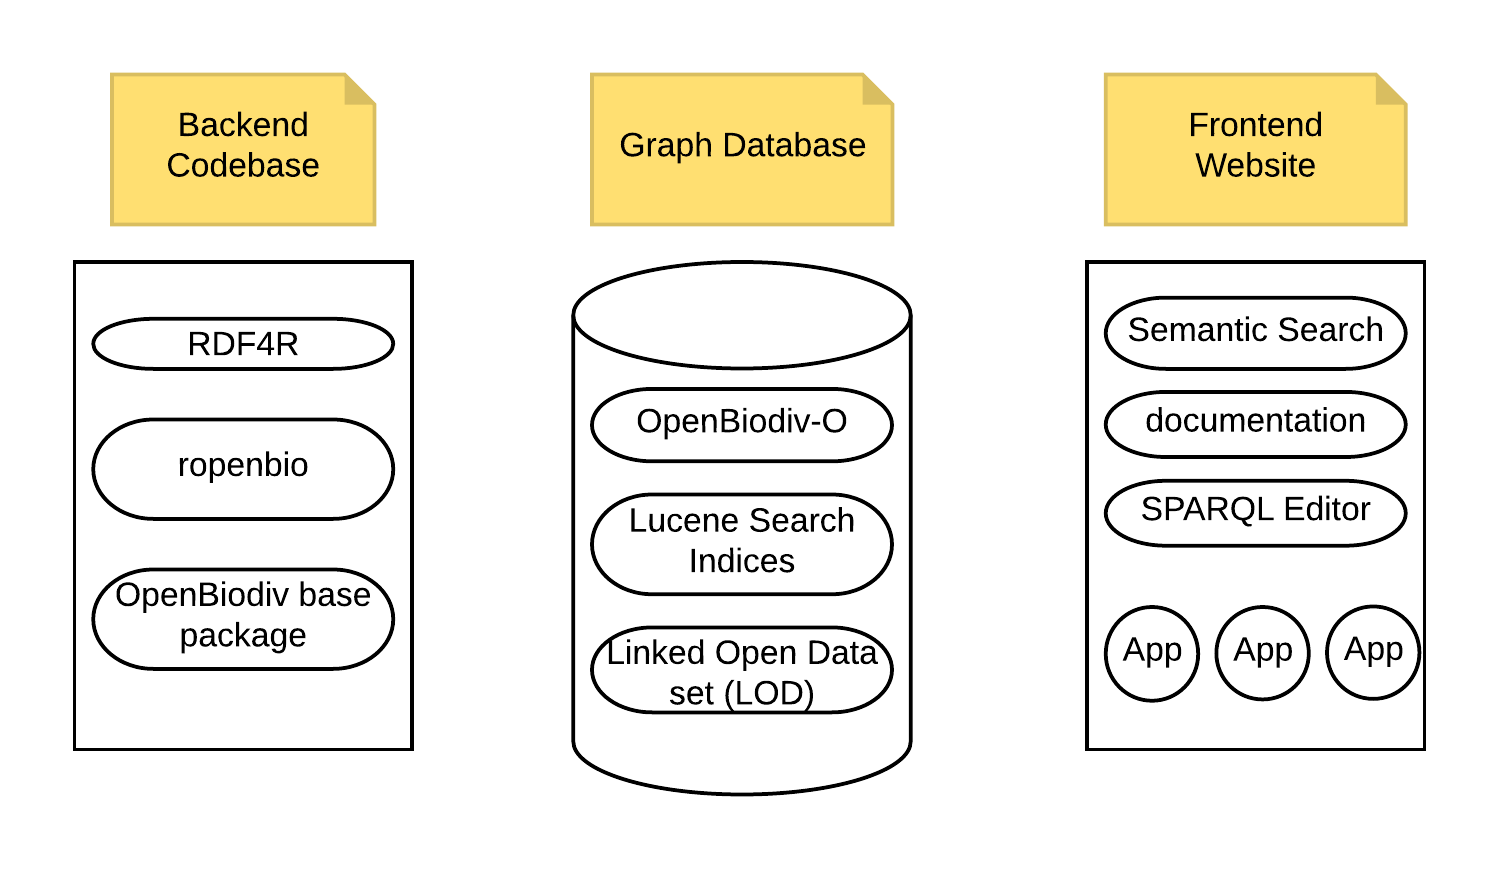
\includegraphics[width=\textwidth]{Figures/components-openbiodiv}
\decoRule
\caption[OpenBiodiv Components]{The components of OpenBiodiv.}
\label{fig:openbiodiv-components}
\end{figure}

\begin{figure}
\centering
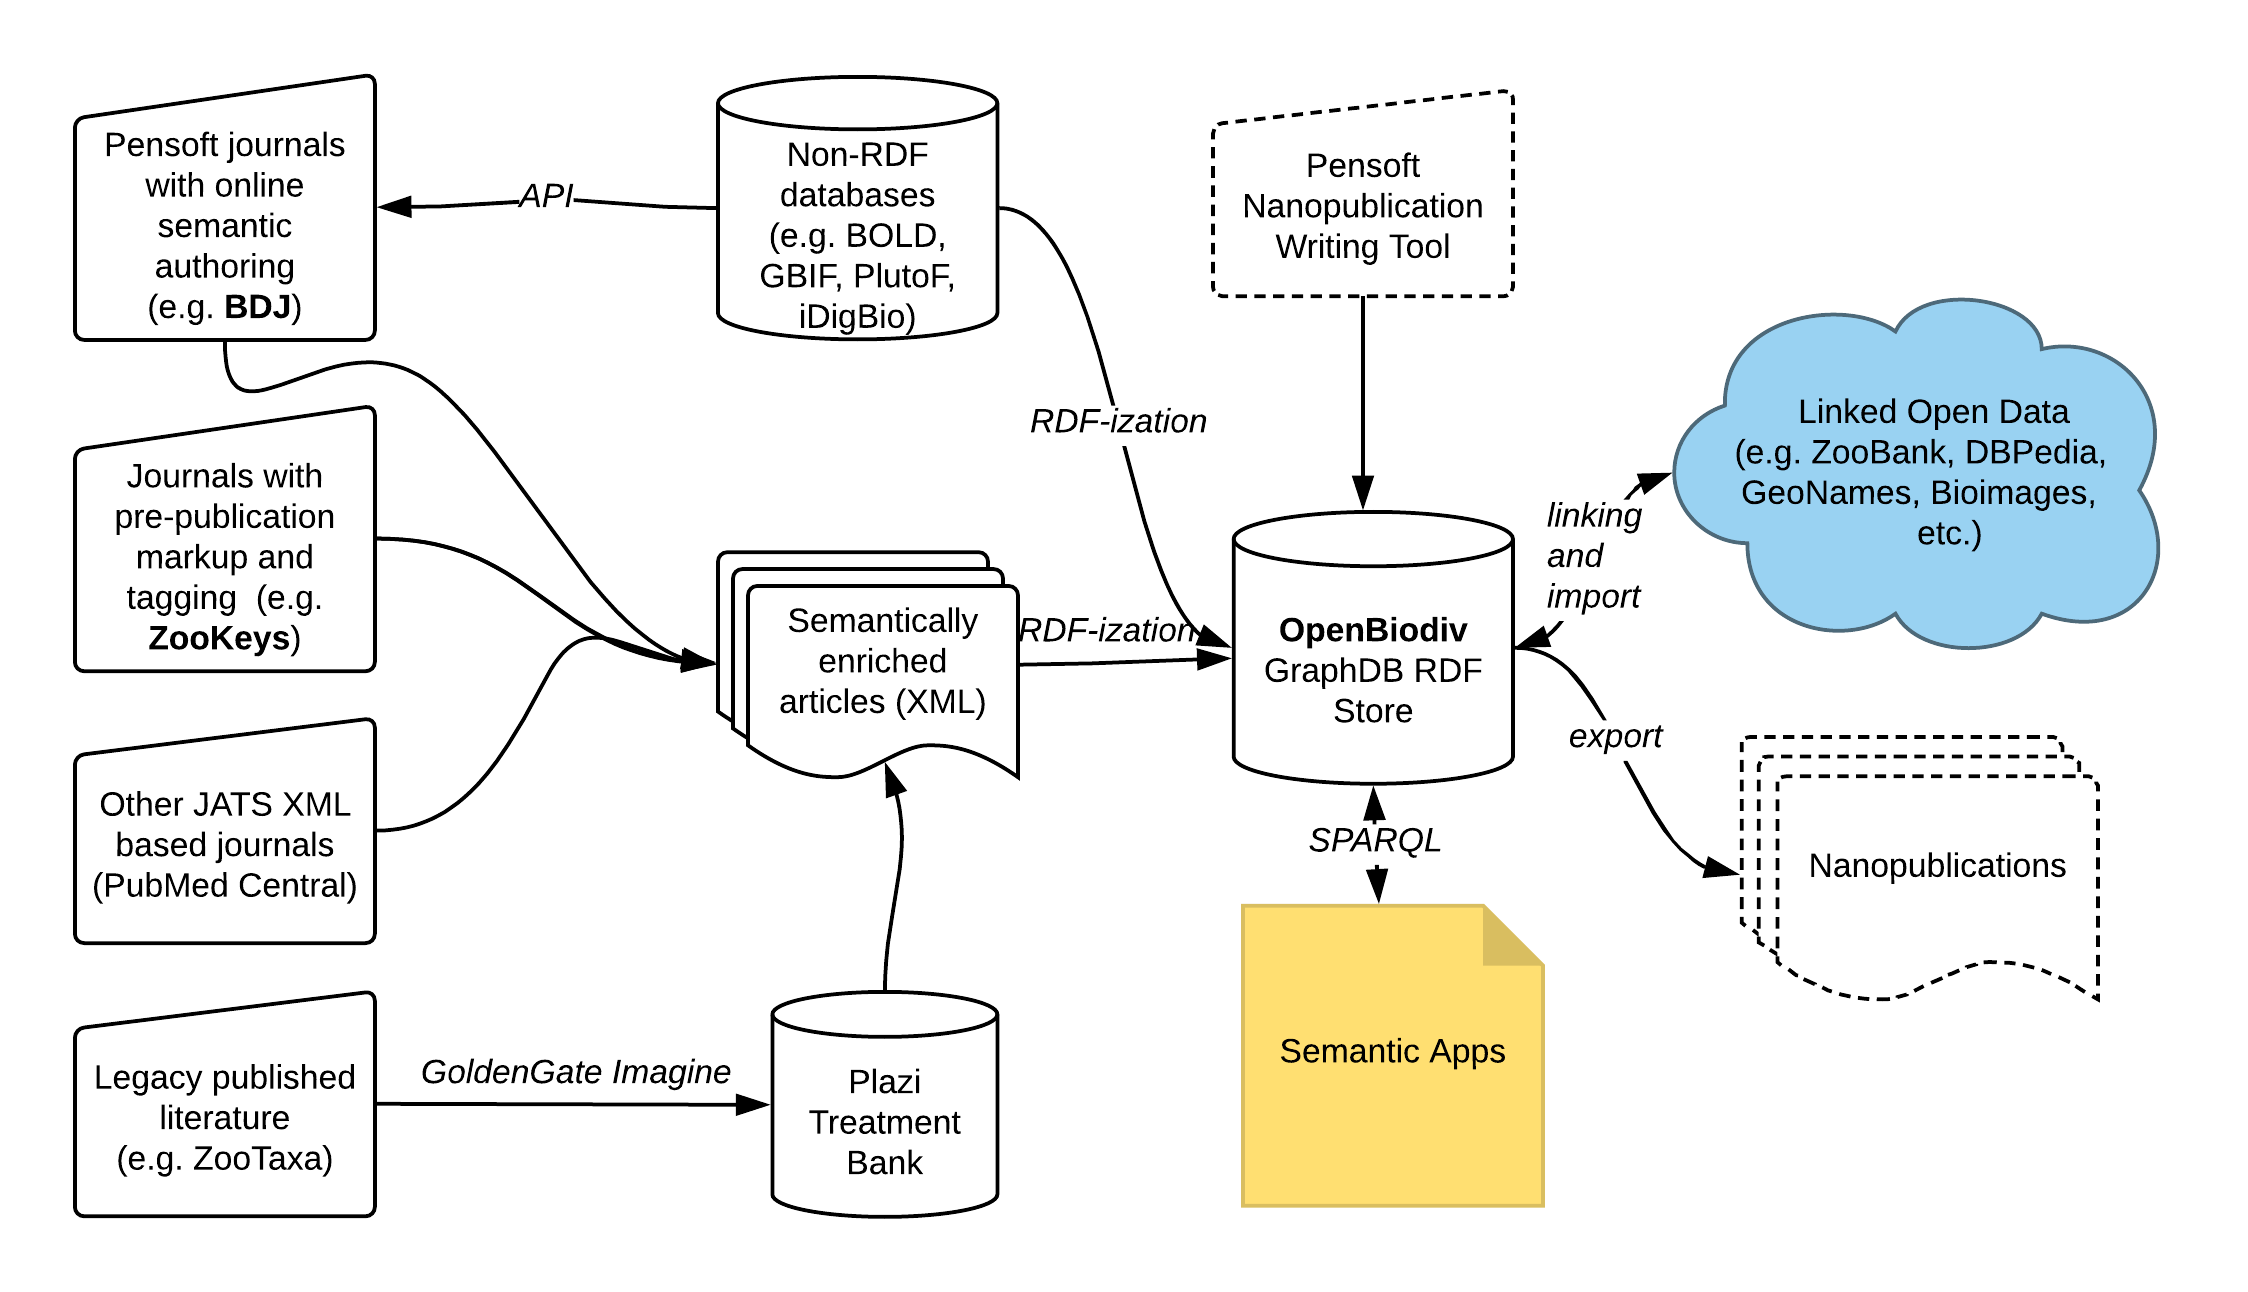
\includegraphics[width=\textwidth]{Figures/openbiodiv-sources}
\decoRule
\caption[OpenBiodiv Components]{Flow of information in the biodiversity data space until it reaches the OpenBiodiv semantic database. Dashed lines are components that have not been implemented yet.
}
\label{fig:openbiodiv-sources}
\end{figure}

\section{Semantic Graph Database}

A primary output of the OpenBiodiv effort is the creation of a semantic database based on knowledge extracted from the archives of Pensoft and Plazi and GBIF's taxonomic backbone and accessible under \url{http://graph.openbiodiv.net/}. A discussion of the components of the database follows.

\subsection{OpenBiodiv ontology (OpenBiodiv-O)}

The central result of the OpenBiodiv effort is the creation of a formal domain model of biodiversity publishing, the ontology OpenBiodiv-O (\cite{senderov_openbiodiv_2017}). The source code of the ontology and accompanying documentation can be accessed under \url{https://github.com/vsenderov/openbiodiv-o}. A detailed discussion is presented in Chapter~\ref{chapter-ontology}.

\subsection{OpenBiodiv Linked Open Dataset (OpenBiodiv-LOD)}

Using OpenBiodiv-O and the infrastructure described later in this chapter a dataset incorporating approximately 200 thousand Plazi treatments, five thousand Pensoft articles, as well as GBIF’s taxonomic backbone (over a million names) has been created. The dataset is available online through the workbench of the semantic database \url{http://graph.openbiodiv.net}. It is discussed in detail in Chapter~\ref{chapter-lod}.

\section{Backend}

In order to populate a semantic database it is necessary to create the infrastructure that converts raw data (text, images, data tables, etc.) into a structured semantic format allowing the interlinking of resource identifiers and the answering of complex queries. OpenBiodiv creates new infrastructure and extends existing infrastructure for transforming biodiversity scholarly publications into Resource Description Format (RDF) statements with the help of the components described in this section.

\subsection{RDF4R: R package for working with RDF}

One of the greater technical challenges for OpenBiodiv is the transformation of biodiversity information (e.g. taxonomic names, paper metadata, figures, etc.) stored as semi-structured XML into fully-structured semantic knowledge in the form of RDF. In order to solve this challenge, an R package has been developed that enables the creation, manipulation, and submission and retrieval to and from a semantic database of RDF statements. This package is accessible under an open source license on GitHub under \url{https://github.com/vsenderov/rdf4r}. We describe the package in Chapter~\ref{chapter-rdf4r}.

\subsection{OpenBiodiv Base and ROpenBio}

In combination with the RDF4R package, the code-base is completed by one more R package, \url{ropenbio} and a code-base (OpenBiodiv Base) of scripts and documentation necessary to bootstrap the database. \url{ropenbio} utilizes the RDF4R package to convert semi-structured XML to RDF. It contains the "mappings" necessary for that conversion. It is available under \url{https://github.com/pensoft/ropenbio}. OpenBiodiv Base coordinates the invocation of \url{ropenbio}, contains scripts for the automatic import of new resources, and other housekeeping details. It is available under \url{https://github.com/vsenderov/openbiodiv}. Their usage to generate the OpenBiodiv-LOD is discussed in Chapter~\ref{chapter-lod}.

\subsection{Workflow for converting ecological metadata to a manuscript}  

Ecological Metadata Language (EML) is a popular format for describing ecological datasets (\cite{michener_nongeospatial_1997}). Biodiversity repositories such as GBIF and DataOne make use of this format to describe the datasets that they store. An import pipeline for importing an EML file as a BDJ data paper\footnote{A data paper (\cite{chavan_data_2011}) is a paper in a scholarly (peer-reviewed) journal discussing a scientific dataset.} has been developed as part of OpenBiodiv (\cite{senderov_online_2016}). We describe this workflow in detail in Chapter~\ref{chapter-case-study}. To access the pipeline interactively, go to \url{https://arpha.pensoft.net}, login to the system (registration is free), select ``Start a new manuscript,'' scroll all the way down to ``Import a manuscript,'' and follow the necessary steps to upload an EML and use it as a template for your new manuscript.

\subsection{Workflow for importing specimen data into Biodiversity Data Journal}

One of the important types of biodiversity data is occurrence data---data that documents the presence of a properly taxonomically identified organism at a given location and time. Such data is stored at international repositories such as BOLD, GBIF, PlutoF, and iDigBio. In order to facilitate data publishing, as well as to act as an entry point into OpenBiodiv, a pipeline for importing any occurrence record from these databases into a BDJ taxonomic paper has been developed (\cite{senderov_online_2016}). We describe this workflow in detail in Chapter ~\ref{chapter-case-study}. To access the workflow interactively, go to \url{https://arpha.pensoft.net}, login to the system (registration is free), select "Start a new manuscript," select "Biodiversity Data Journal" as a journal and "Taxonomic Paper" as paper-type and "Create a manuscript." Then, in your new manuscript, expand the "Taxon treatments" section by clicking on the $+$ sign next to it, give a test classification to your treatment (e.g. Animalia), click ``Save'' and you will be presented with a choice of subsections. Click the ``Materials'' section on the left to visualize the workflow. Look at the lower-part of the dialog, where ``You may place multiple ID's...''---this is the part where you select external resource identifiers to be imported to your article.

\section{Frontend}

In addition to providing a searchable database endpoint, a website allowing semantic search and containing specific tasks packaged as apps is being developed (\url{http://openbiodiv.net}). The development of the site extends beyond the scope of the dissertation thesis and is driven by the Pensoft development team. A beta version is already operational Fig.~\ref{fig:website}. A limited discussion is found in Chapter~\ref{webportal}.

\todo{Chapter should be an appendix instead}

\section{IT}

The system is deployed on a Debian GNU+Linux virtual machine. GraphDB runs with a 20 GB heap file and with the RDFS-Plus Optimized rule set\footnote{This is necessitated by the fact that we reached a performance bottleneck the OWL inference. Discussed in Chapter~\ref{chapter-lod}}.  Continuous operation is ensured by the automatic execution of scripts from the \url{run} directory of OpenBiodiv Base.

\begin{figure}
\centering
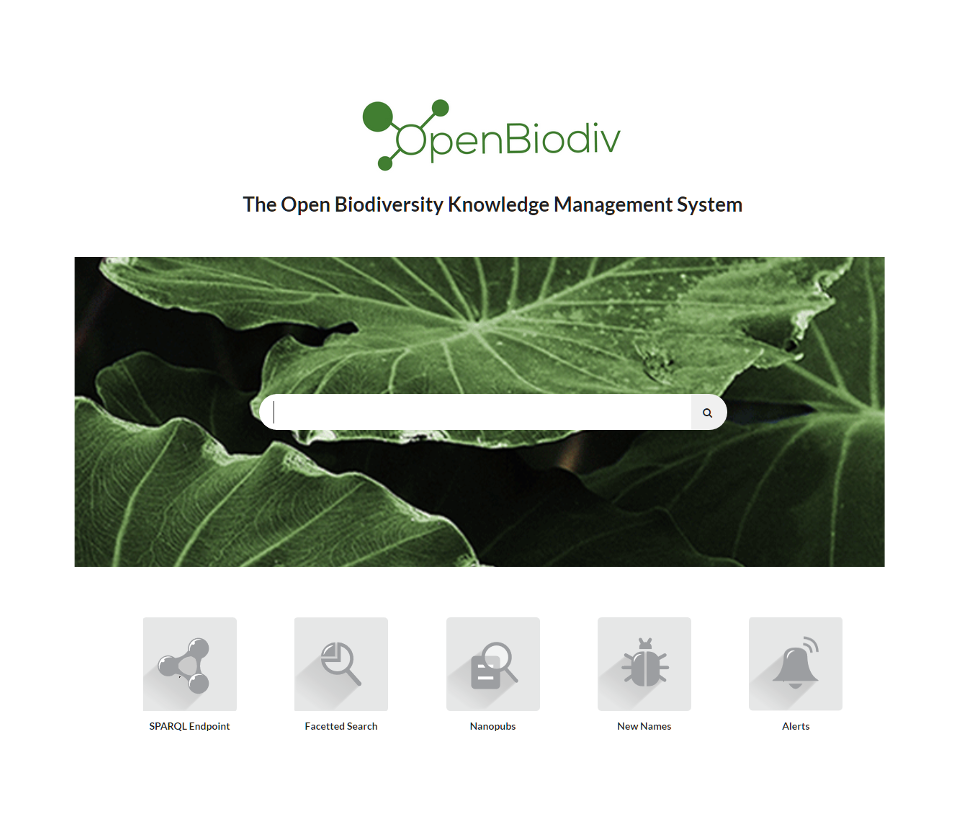
\includegraphics[width=\textwidth]{Figures/openbiodiv-webpage}
\decoRule
\caption[OpenBiodiv Website]{Beta version of the OpenBiodiv website together with sample app icons.}
\label{fig:website}
\end{figure}



\chapter{The OpenBiodiv Ontology}

\label{chapter-ontology}

OpenBiodiv lifts biodiversity information from scholarly publications and academic databases into a computable semantic form.  In this chapter, we introduce OpenBiodiv-O (\cite{senderov_openbiodiv-o:_2018}), the ontology forming the knowledge and inferencing model of OpenBiodiv. OpenBiodiv-O provides a conceptual model of the structure of a biodiversity publication and the development of related taxonomic concepts. We first introduce the modeled domain in Domain Conceptualization and then formalize it in Results. 

By developing an ontology focusing on biological taxonomy, our intent is to provide an ontology that fills in the gaps between ontologies for biodiversity resources such as Darwin-SW and semantic publishing ontologies such as the ontologies comprising the SPAR Ontologies. We take the view that it is advantageous to model the taxonomic process itself rather than any particular state of knowledge.

The source code and documentation are available under the CC BY license\footnote{Creative Commons Attribution 4.0 International Public License.} from GitHub\footnote{\href{https://github.com/vsenderov/openbiodiv-o/blob/master/LICENSE.md}{https://github.com/vsenderov/openbiodiv-o}}. We start by introducing the domain of biological taxonomy and the related biodiversity sciences.

\section{Domain Conceptualization}

Biological taxonomy is a very old discipline dating back possibly to Aristotle, whose fundamental insight was to group living things in a hierarchy (\cite{manktelow_history_2010}). The discipline took its modern form after Carl Linnaeus (1707 - 1778). In his \emph{Systema Naturae} Linnaeus proposed to group organisms into \emph{kingdoms, classes, orders, genera}, and \emph{species} bearing latinized scientific names with a strictly prescribed syntax. Linnaeus listed possible alternative names and gave a characteristic description of the groups (\cite{linnaeus_systema_1758}). These groups are called \emph{taxa}, which is a Greek word for \emph{arrangement}. The hierarchy that taxa form is called taxonomy. The etymology of the word is Greek and roughly translates to \emph{method of arranging}. Note the polysemy here: the science of biological taxonomy is called taxonomy as is the arrangement of taxa itself. We believe, however, that it is sufficiently clear from context what is meant by "taxonomy" in any particular usage throughout this thesis.

Even though Linnaeus and his colleagues may have hoped to describe life on Earth during their lifetimes, we now know that there are millions of species still undiscovered and undescribed (\cite{trontelj_cryptic_2009}). On the other hand, our understanding of species and higher-rank taxonomic concepts changes as evolutionary biology advances (\cite{mallet_species_2001}). Therefore, an accurate and evolutionarily reliable description of life on Earth is a perpetual process and cannot be completed with a single project that can be converted into an ontology. Thus, our aim is not to create an ontology capturing a fixed view of biological taxonomy, but to create an ontology of the taxonomic process. The ongoing use of this ontology will enable the formal description of taxonomic biodiversity knowledge at any given point in time. In the following paragraphs, we introduce what the taxonomic process entails and reflect on the resources that need modeling.

An examination of the taxonomic process reveals that taxonomy works by employing the scientific method: researchers examine specimens and, based on the phenotypic and genetic variation that they observe, form a hypothesis (\cite{deans_time_2012}). This hypothesis may be called a taxonomic concept, a potential taxon, a species hypothesis (\cite{berendsohn_concept_1995}), or an operational taxonomic unit (OTU, \cite{sokal_principles_1963}) in the case of a numerically delimited taxon.

A taxonomic concept describes the allowable phenotypic, genomic, or other variation within a taxon by designating type specimens and describing characters explicitly. It is a valid falsifiable scientific claim as it needs to fulfill certain verifiable evolutionary requirements. For example, a species-rank taxonomic hypothesis needs to fit our current understanding of species (species concept,  \cite{mallet_species_2001}). More generally, the aspiration is that species concepts are adequate and give certain tangible criteria for species delimitation. However, valid scientific discussions continue about concept adequacy. The discussions are nuanced because they often draw on different conceptions of the relative weight of certain evolutionary phenomena. This leads to having quite a few different species concepts---morphological, ecological, phylogenetic, genomic, biological, etc. (\cite{mallet_species_2001}). Nevertheless, if we fix a species concept---let us say we take the biological species concept---we can falsify any given species-rank taxonomic hypothesis against our fixed species concept.

Similarly, hypotheses of higher rank (representing upper levels of the taxonomic hierarchy) also need to fulfill certain evolutionary requirements. For example, a modern genus concept requires all species assigned to it to be descendants of a separate lineage and to form a monophyletic clade.

The ranks (taxonomy hierarchy levels) are not completely fixed. The usage of lower ranks (species, genus, family, order) is governed by international Codes (\cite{international_commission_on_zoological_nomenclature_international_1999,mcneill_international_2012}). In the example of Linnaeus' ranks, each organism is first a member of its species, then genus, then order, then class, and finally kingdom. Which specific ranks a given taxonomic study employs is dependent on the field (e.g. botany vs. zoology), on the particular author, on the level of taxonomic resolution required, as well as on the history of classifying in that particular group.

Once the researchers have formed their concept, it must be published in a scientific outlet (journal or book). The biological Codes put some requirements and recommendations aimed at ensuring the quality of published research but ultimately it is a democratic process guaranteeing that everyone may publish taxonomic concepts provided they follow the rules of the Codes. This means that in order to create a knowledge base of biodiversity, we need to be able to mine taxonomic papers from legacy and modern journals and books.

As a first good approximation, a taxonomic concept is based on a number of specimens or occurrences that are listed in a section usually called "Materials Examined." In general terms, we can say that a sighting of a living thing, i.e. an organism, at a given location and at a given time is referred to as an occurrence, and a voucher for this occurrence (e.g. the sampling of the organism itself) is referred to as a specimen (\cite{baskauf_darwin-sw:_2016}). Moreover, a taxonomic article may include other specialized sections such as the Checklist section, where one may list all taxa (in fact: the taxonomic concepts for those taxa) for organisms observed in a given region.

Typically, the information content of a treatment consists of several units. First, we have the aforementioned nomenclatural information that pertains to the scientific name---its authorship, etymology, related names, etc. Then, we have the taxonomic concept information that can be considered to have two components, as well: the first one is the intensional component of the taxonomic concept made up mostly of \emph{traits} or \emph{characters}. Traits are an explicit definition of the allowable variation (e.g. phenotypic, genomic, or ecological) of the organisms that make up the taxon. For example, we can define the order of spiders, Araneae, to be the class of organisms that have specialized appendages used for sperm transfer called pedipalps (\cite{platnick_cladograms_2001}). Knowledge of this kind is found in the Diagnosis, Description, Distribution and other subsections of the treatment.

Non-traditionally delimited taxonomic hypotheses are called \emph{operational taxonomic units} (OTU's). In the case of genomic delimitation, sometimes the concepts are published directly as database entries and not as Code-compliant taxonomic articles (\cite{page_dna_2016}). A genomic delimitation can, for example, be based on a barcode sequence and on a statistical clustering algorithm specifying the allowable sequence variability that an organism can possess in order to be considered part of the barcode sequence-bearing operational taxonomic unit. However, as, in the general case, we don't have a Linnaean name or a morphological description for an operational taxonomic unit, we refer to it as a \emph{dark taxon} (\cite{page_dna_2016}). The term "dark" is, however, usually reserved for concepts at lower ranks. Operational taxonomic units are published, for example, in the form of \emph{barcode identification numbers} (BIN's) in the Barcode of Life Data Systems (BOLD, \cite{ratnasingham_dna-based_2013}), or as \emph{species hypotheses} in Unified system for the DNA based fungal species linked to the classification (UNITE, \cite{koljalg_towards_2013}).

The second part of the information content of a taxonomic concept is the ostensive component: a listing of some (but not necessarily all) of the organisms that belong to the taxonomic concept. This information is found in the Materials Examined subsection of the treatment.

Finally, the relationships between taxonomic concepts---simple hierarchical (\emph{is a}) or more fine-grained Region Connection Calculus 5 (RCC-5, \cite{franz_perspectives:_2009, franz_two_2016})---can be both intensionally defined in the nomenclature section or ostensively inferred from the Materials Examined. However, given the customary idiosyncrasies of biological descriptions, providing an initial set of RCC-5 relationships for a machine reasoner to work with often requires expert assessment and cannot be easily lifted from the text.

Thus, in order to model the taxonomic process, our ontology models scholarly taxonomic papers, database entries, agents responsible for their creation, treatments, taxonomic concepts, scientific names, occurrence and specimen information, other entities (e.g. ecological, geographical) part-taking in the taxonomic process, as well as relationships among these.



\subsection*{Previous work}

In the biomedical domain there are well-established efforts to extract information and discover knowledge from literature (\cite{momtchev_expanding_2009, williams_open_2012, rebholz-schuhmann_facts_2005}). The biodiversity domain, and in particular biological systematics and taxonomy (from here on in this thesis referred to as \emph{taxonomy}), is also moving in the direction of semantization of its research outputs (\cite{kennedy_scientific_2005,penev_fast_2010, tzitzikas_integrating_2013}). The publishing domain has been modeled through the Semantic Publishing and Referencing Ontologies (SPAR Ontologies, \cite{peroni_semantic_2014}). The SPAR Ontologies are a collection of ontologies incorporating---amongst others---FaBiO, the FRBR-aligned Bibliographic Ontology (\cite{peroni_fabio_2012}), and DoCO, the Document Component Ontology (\cite{constantin_document_2016}). The SPAR Ontologies provide a set of classes and properties for the description of general-purpose journal articles, their components, and related publishing resources. Taxonomic articles and their components, on the other hand, have been modeled through the TaxPub XML Document Type Definition (DTD, also referred to loosely as XML schema) and the Treatment Ontologies (\cite{catapano_taxpub:_2010,catapano_treatment_2016}). While TaxPub is the XML-schema of taxonomic publishing for several important taxonomic journals (e.g. ZooKeys, Biodiversity Data Journal), the Treatment Ontologies are still in development and have served as a conceptual template for OpenBiodiv-O.

Taxonomic nomenclature is a discipline with a very long tradition. It transitioned to its modern form with the publication of the Linnaean System (\cite{linnaeus_systema_1758}). Already by the beginning of the last century, there were hundreds of vocabulary terms (e.g. \emph{types}) (\cite{witteveen_naming_2015}). At present the naming of organismal groups is governed by by the International Code of Zoological Nomenclature (ICZN, \cite{international_commission_on_zoological_nomenclature_international_1999}) and by the International Code of Nomenclature for algae, fungi, and plants (Melbourne Code, \cite{mcneill_international_2012}). Due to their complexity (e.g. ICZN has 18 chapters and 3 appendices), it proved challenging to create a top-down ontology of biological nomenclature. Example attempts include the relatively complete NOMEN ontology (\cite{dmitriev_nomen_2017}) and the somewhat less complete Taxonomic Nomenclatural Status Terms (TNSS, \cite{morris_taxonomic_nodate}).

There are several projects that are aimed at modeling the broader biodiversity domain conceptually. Darwin Semantic Web (Darwin-SW, \cite{baskauf_darwin-sw:_2016}) adapts the previously existing Darwin Core (DwC) terms (\cite{wieczorek_darwin_2012}) as RDF. These models deal primarily with organismal occurrence data.

Modeling and formalization of the strictly taxonomic domain has been discussed by \cite{berendsohn_concept_1995} and later, e.g., in \cite{franz_perspectives:_2009,sterner_taxonomy_2017}. Noteworthy efforts are the XML-based Taxonomic Concept Transfer Schema (\cite{taxonomic_names_and_concepts_interest_group_taxonomic_2006}) and a now defunct Taxon Concept ontology (\cite{devries_taxon_nodate}).

\section{Methods}

OpenBiodiv-O is expressed in Resource Description Framework (RDF). At the onset of the project, a consideration was made to use RDF in favor of a more complex data model such as Neo4J's (\cite{senderov_open_2016}). The choice of RDF was made in order to be able to incorporate the multitude of existing domain ontologies into the overall model.

To develop the conceptualization of the taxonomic process and then the ontology we utilized the following process: (1) domain analysis and identification of important resources and their relationships; (2) analysis of existing data models and ontologies and identification of missing classes and properties for the successful formalization of the domain.

The formal structure of the ontology is specified by employing the RDF Schema (RDFS) and the Web Ontology Language (OWL). It is encoded as a part of a literate programming (\cite{knuth_literate_1984}) document in RMarkdown format titled ``OpenBiodiv Ontology and Guide''\footnote{\href{http://openbiodiv.net/ontology}{http://openbiodiv.net/ontology}}. The statements have been extracted from the RMarkdown file via \emph{knitr} and are provided here as an appendix. It is also possible to request the ontology via Curl from its endpoint with the indication of {\tt content-type: application/rdf+xml}. The vocabularies can be found as additional appendices, Taxonomic Statuses and RCC-5, and on the GitHub page\footnote{\href{https://github.com/vsenderov/openbiodiv-o}{https://github.com/vsenderov/openbiodiv-o}}.

A dataset (OpenBiodiv-LOD, will be described in detail in the next Chapter) from Pensoft's journals, Plazi's treatments, and GBIF's taxonomic backbone has been generated with \mbox{OpenBiodiv-O} and can be found at the SPARQL Endpoint \footnote{\href{http://graph.openbiodiv.net/}{http://graph.openbiodiv.net/}}. The endpoint is also accessible from the website\footnote{\href{http://openbiodiv.net/}{http://openbiodiv.net/}}, under ``SPARQL Endpoint.'' Demos are available as ``Saved Queries'' from the workbench.

\section{Results}

We understand OpenBiodiv-O to be the \emph{shared formal specification of the conceptualization} (\cite{gruber_translation_1993,obitko_translations_2007,staab_handbook_2009}) that we have introduced in Background. OpenBiodiv-O describes the structure of this conceptualization, not any particular state of it.

There are several domains in which the modeled resources fall. The first one is the scholarly biodiversity publishing domain. The second domain is that of taxonomic nomenclature. The third domain is that of broader taxonomic (biodiversity) resources (e.g. taxonomic concepts and their relationships, species occurrences, traits). To combine such disparate resources together we rely on SKOS \cite{miles_skos_nodate}. Unless otherwise noted, the default namespace of the classes and properties for this paper is \url{<http://openbiodiv.net/>}. The prefixes discussed here are listed at the beginning of the ontology source code.

\subsection{Semantic Modeling of the Biodiversity Publishing Domain}

An article as such may be represented by a set of metadata, while its content consists of article components such as sections, tables, figures and so on (\cite{peroni_example_2015}).

To accommodate the specific needs of scholarly biodiversity publishing, we introduce a new class for taxonomic articles, Taxonomic Article ({\tt :TaxonomicArticle}), new classes for specific subsections of the taxonomic
article such as Taxonomic Treatment, Taxonomic Key, and Taxonomic Checklist, and a new class, Taxonomic Name Usage ({\tt :TaxonomicNameUsage}), for the mentioning of a taxonomic name (see next subsection) in an article. These new classes are summarized in Table~\ref{bibliographic_classes}.

\begin{table}[h!]
\caption{New biodiversity publishing classes introduced.}
      \begin{tabular}{cc}
        \hline
          Class QName             & Comment\\  \hline
  {\tt :Treatment}                & section of a taxonomic article\\
  {\tt :NomenclatureSection}      & subsection of Treatment\\
  {\tt :NomenclatureHeading}      & contains a nomenclatural act \\
  {\tt :NomenclatureCitationList} & list of citations of related concepts\\
  {\tt :MaterialsExamined}        & list of examined specimens\\
  {\tt :BiologySection}           & subsection of Treatment\\
  {\tt :DescriptionSection}       & subsection of Treatment\\
  {\tt :TaxonomicKey}             & section with an identification key\\
  {\tt :TaxonomicChecklist}       & section with a list of taxa for a region\\ 
  {\tt :TaxonomicNameUsage}       & mention of a taxonomic name\\ \hline

      \end{tabular}
      \label{bibliographic_classes}
\end{table}

The classes from this subsection are based on the TaxPub XML Document Type Definition (DTD, also referred to loosely as XML schema, \cite{catapano_taxpub:_2010}), on the structure of Biodiversity Data Journal's
taxonomic paper (\cite{smith_beyond_2013}), and and on the Treatment Ontologies (\cite{catapano_treatment_2016}).

Furthermore, we introduce two properties: \emph{contains} ({\tt :contains}) and \emph{mentions} ({\tt :mentions}). \emph{contains} is used to link parts of the article together and \emph{mentions} links parts of the article to other concepts.

A graphical representation of the relationships between instances of the publishing-related classes that OpenBiodiv introduces is to be found in the diagram in Fig.~\ref{taxonomic-article-diagram}.

\begin{figure}[h!]
	\centering
	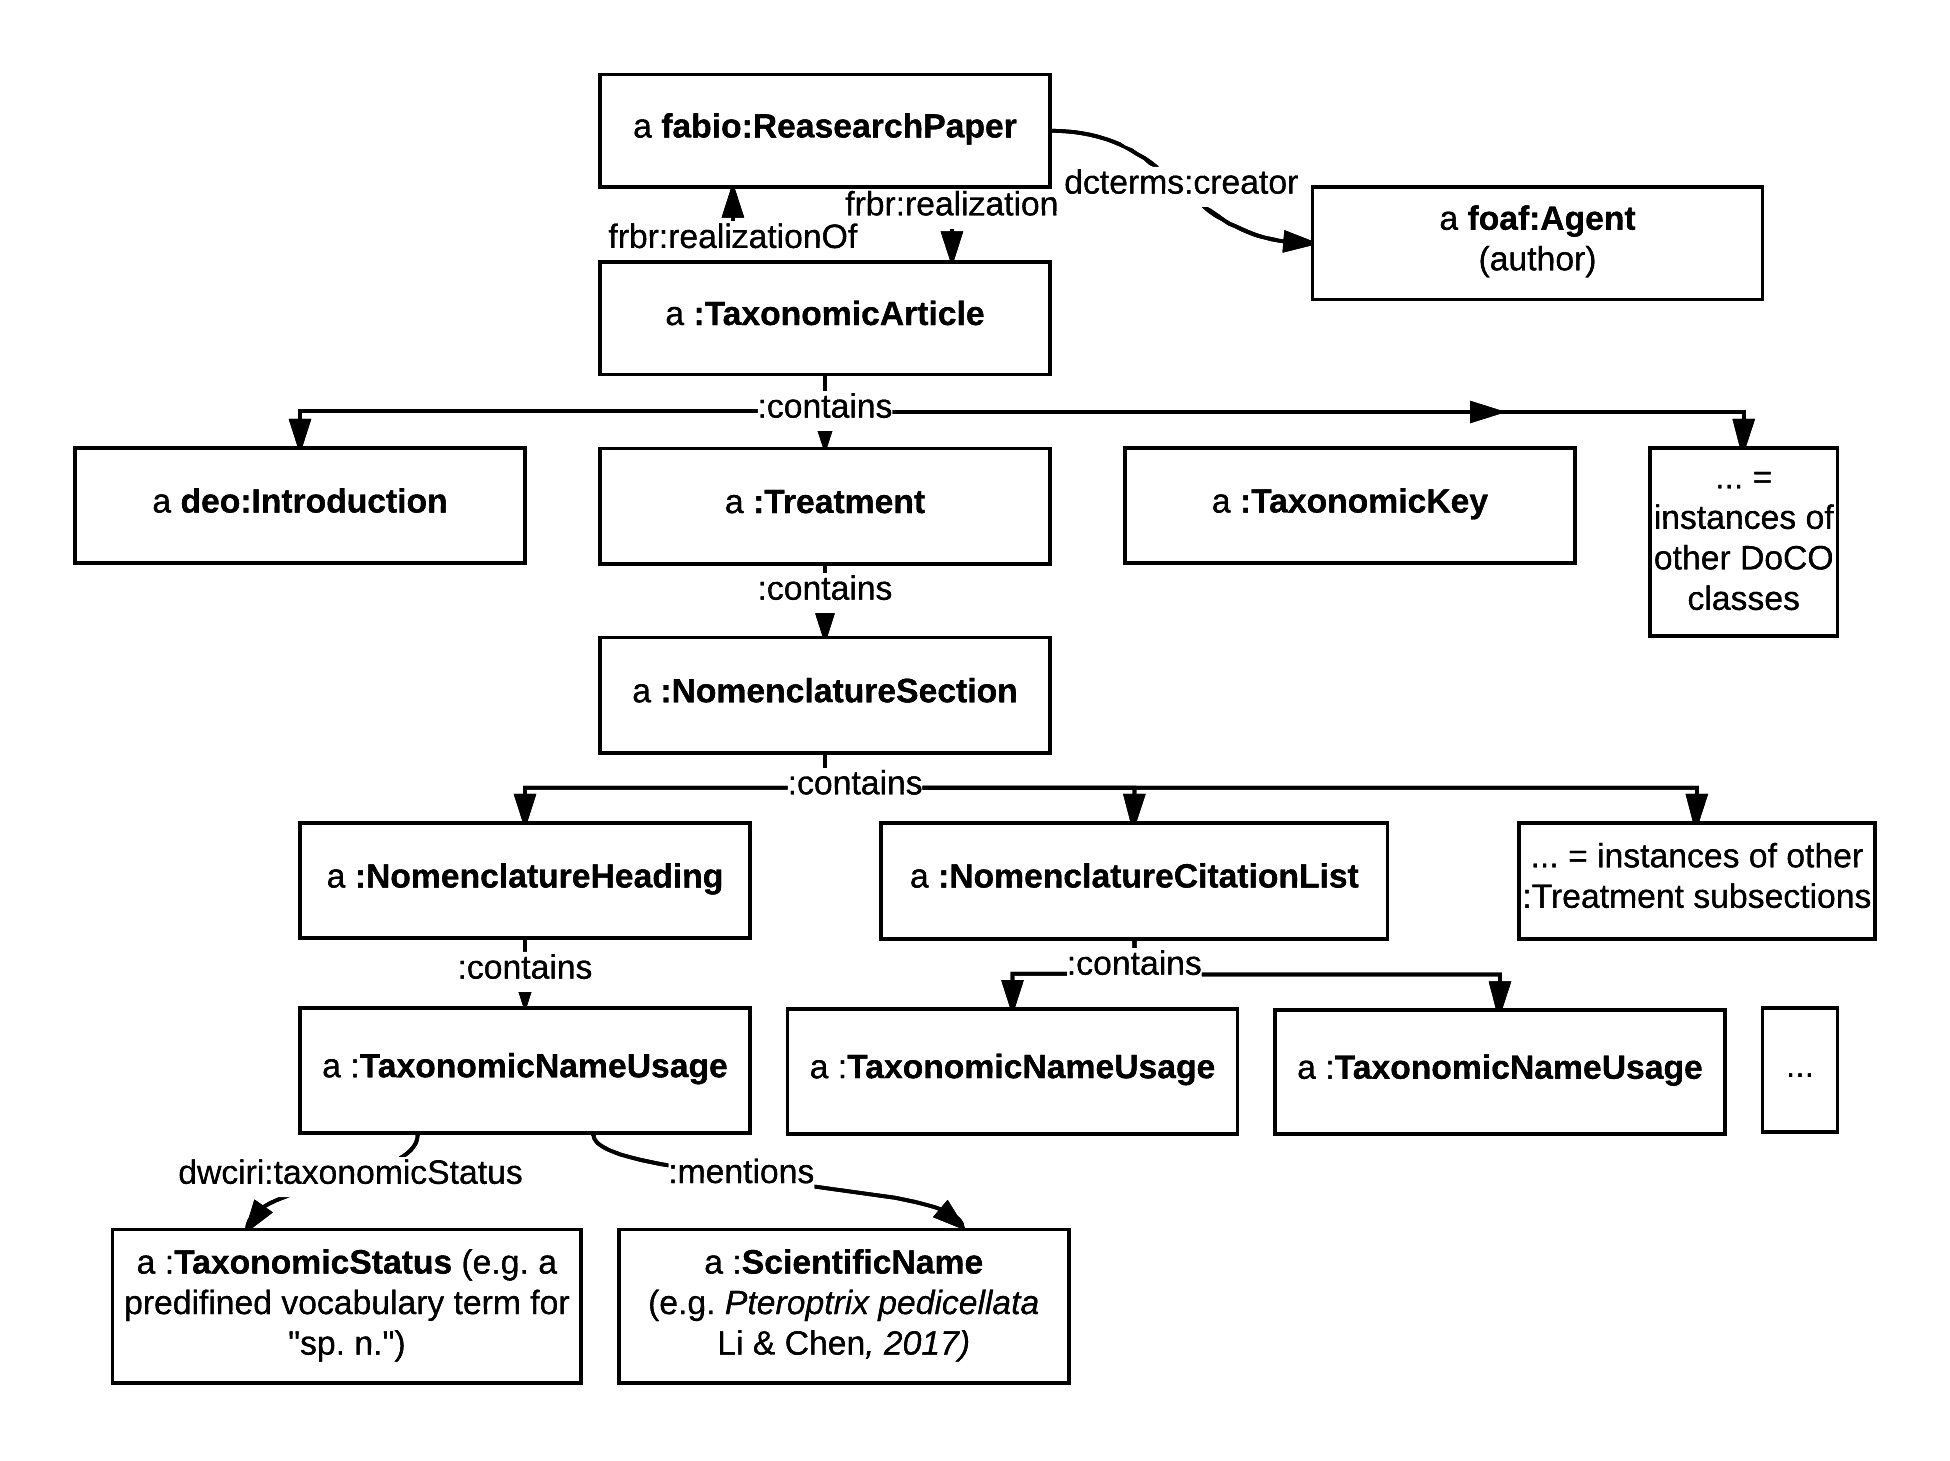
\includegraphics[width=\textwidth]{Figures/taxonomic-article-diagram}
	\decoRule
  \caption[Taxonomic article diagram.]{A graphical representation of the relationships between instances of the publishing-related classes that OpenBiodiv introduces.}
  \label{taxonomic-article-diagram}
\end{figure}

\subsubsection{Semantics, alignment, and usage}

Our bibliographic model has the Semantic Publishing and Referencing Ontologies (SPAR Ontologies) at its core with a few extensions that we have written to accommodate for taxonomic elements. The SPAR Ontologies' FRBR-aligned Bibliographic Ontology (FaBiO) uses the Functional Requirements for Bibliographic Records (FRBR, \cite{tillett_conceptual_2003}) model to separate publishable items into less or more abstract classes. We deal primarily with the Work class, i.e. the conceptual idea behind a publishable item (e.g. the story of ``War and Peace'' as thought up by Leo Tolstoy), and the Expression class, i.e. a version of record of a Work (e.g. ``War and Peace,'' paperback edition by Wordsworth Classics).

Taxonomic Article is a subclass of FaBiO's Journal Article. Furthermore Journal Article is a FRBR Expression. This implies that taxonomic articles are FRBR expressions as well. This has important implications later on when discussing taxonomic concept labels. Also, it means that we separate the abstract properties of an article (in a FaBiO Research Paper instance, which is a Work) from the version of record (in a Taxonomic Article, an Expression).

The taxonomic-specific section and subsection classes are introduced as subclasses of Discourse Element Ontology's (DEO) Discourse Element ({\tt deo:DiscourseElement},  \cite{constantin_document_2016}). So is the class Mention ({\tt :Mention}), meant to represent an area of a document that can be considered a mention of something. This class, and the corresponding property, \emph{mentions}, are inspired by {\tt pext:Mention} and its corresponding property from PROTON (\cite{damova_mapping_2010}). The redefinition is necessary by the fact in OpenBiodiv-O they possess a slightly different semantics and a different placement in the upper-level hierarchy. We then introduce Taxonomic Name Usage as a subclass of Mention.

This placement of the document component classes that we've introduced in Discourse Element means that they ought to be used exactly in the same way as one would use the other discourse elements from DEO and DoCO (analogous to e.g. {\tt deo:Introduction}). Note: DEO is imported by DoCO. Figs.~\ref{example-article-metadata} and \ref{example-article-structure} give example usage in Turtle illustrating these ideas. A caveat here is that while the SPAR Ontologies use {\tt po:contains} in their examples, we use \emph{contains}, which is a subproperty of {\tt po:contains} with the additional property of being transitive. We believe this definition is sensible as surely a sub-subcomponent is contained in a component. All other aspects of expressing a taxonomic article in RDF according to OpenBiodiv-O are exactly the same as according to the SPAR Ontologies.

\begin{figure}[h!]
	\centering
	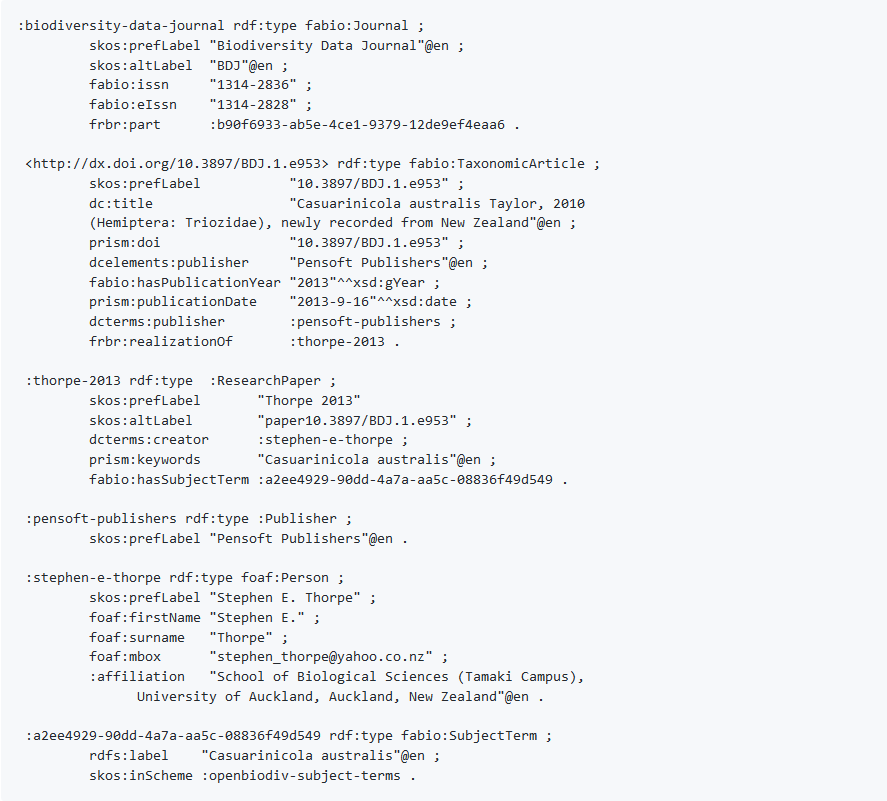
\includegraphics[width=\textwidth]{Figures/example-article-metadata}
	\decoRule
  \caption[Example article metadata.]{This example shows how to express the metadata of a taxonomic article with the SPAR Ontologies' model and the classes that OpenBiodiv defines. The code is in Turtle.}
  \label{example-article-metadata}
\end{figure}

\begin{figure}[h!]
  \centering
  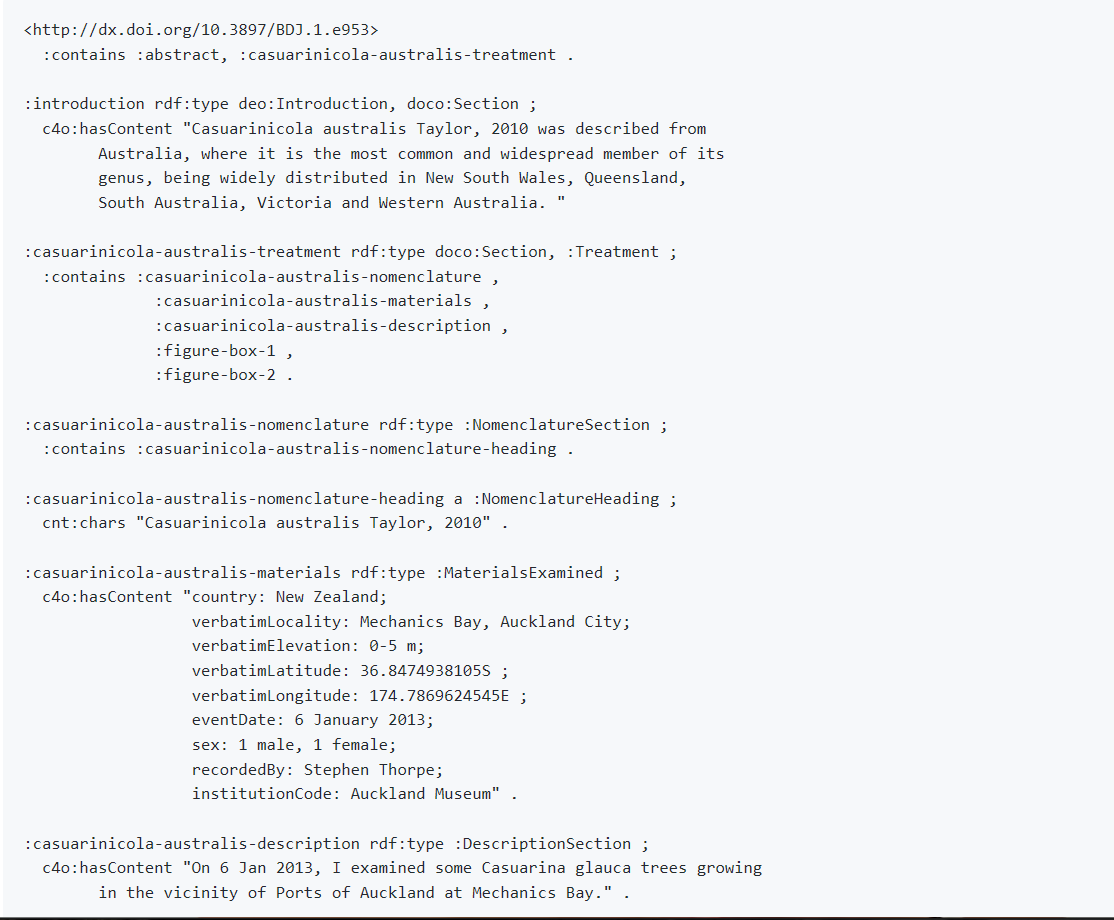
\includegraphics[width=\textwidth]{Figures/example-article-structure}
  \decoRule
  \caption[Example article structure.]{This examples shows how to express the article structure with the help of {\tt :contains}. The code is in Turtle.}
  \label{example-article-structure}
\end{figure}


\subsection{Semantic modeling of biological nomenclature}

While NOMEN and TNSS (introduced in subsection ``Previous work'') take a top-down approach of modeling the nomenclatural Codes, OpenBiodiv-O takes a bottom-up approach of modeling the use of taxonomic names in articles. Where possible we align OpenBiodiv-O classes to NOMEN.

Based on the need to accommodate taxonomic concepts, we have defined the class hierarchy of taxonomic names found in Fig. \ref{taxonomic-name-class-hierarchy-diagram}. Furthermore, we have introduced the class Taxonomic Name Usage ({\tt :TaxonomicNameUsage}). Taxonomic name usages have been discussed widely in the community (e.g. in \cite{pyle_taxonomic_2016}); however, the meaning of term remains vague. The abbreviation TNU is used interchangeably for ``taxon name usage'' and for ``taxonomic name usage.'' In OpenBiodiv-O, a taxonomic name usage is the mentioning of a taxonomic name in the text, optionally followed by a taxonomic status.

\begin{figure}[h!]
  \centering
  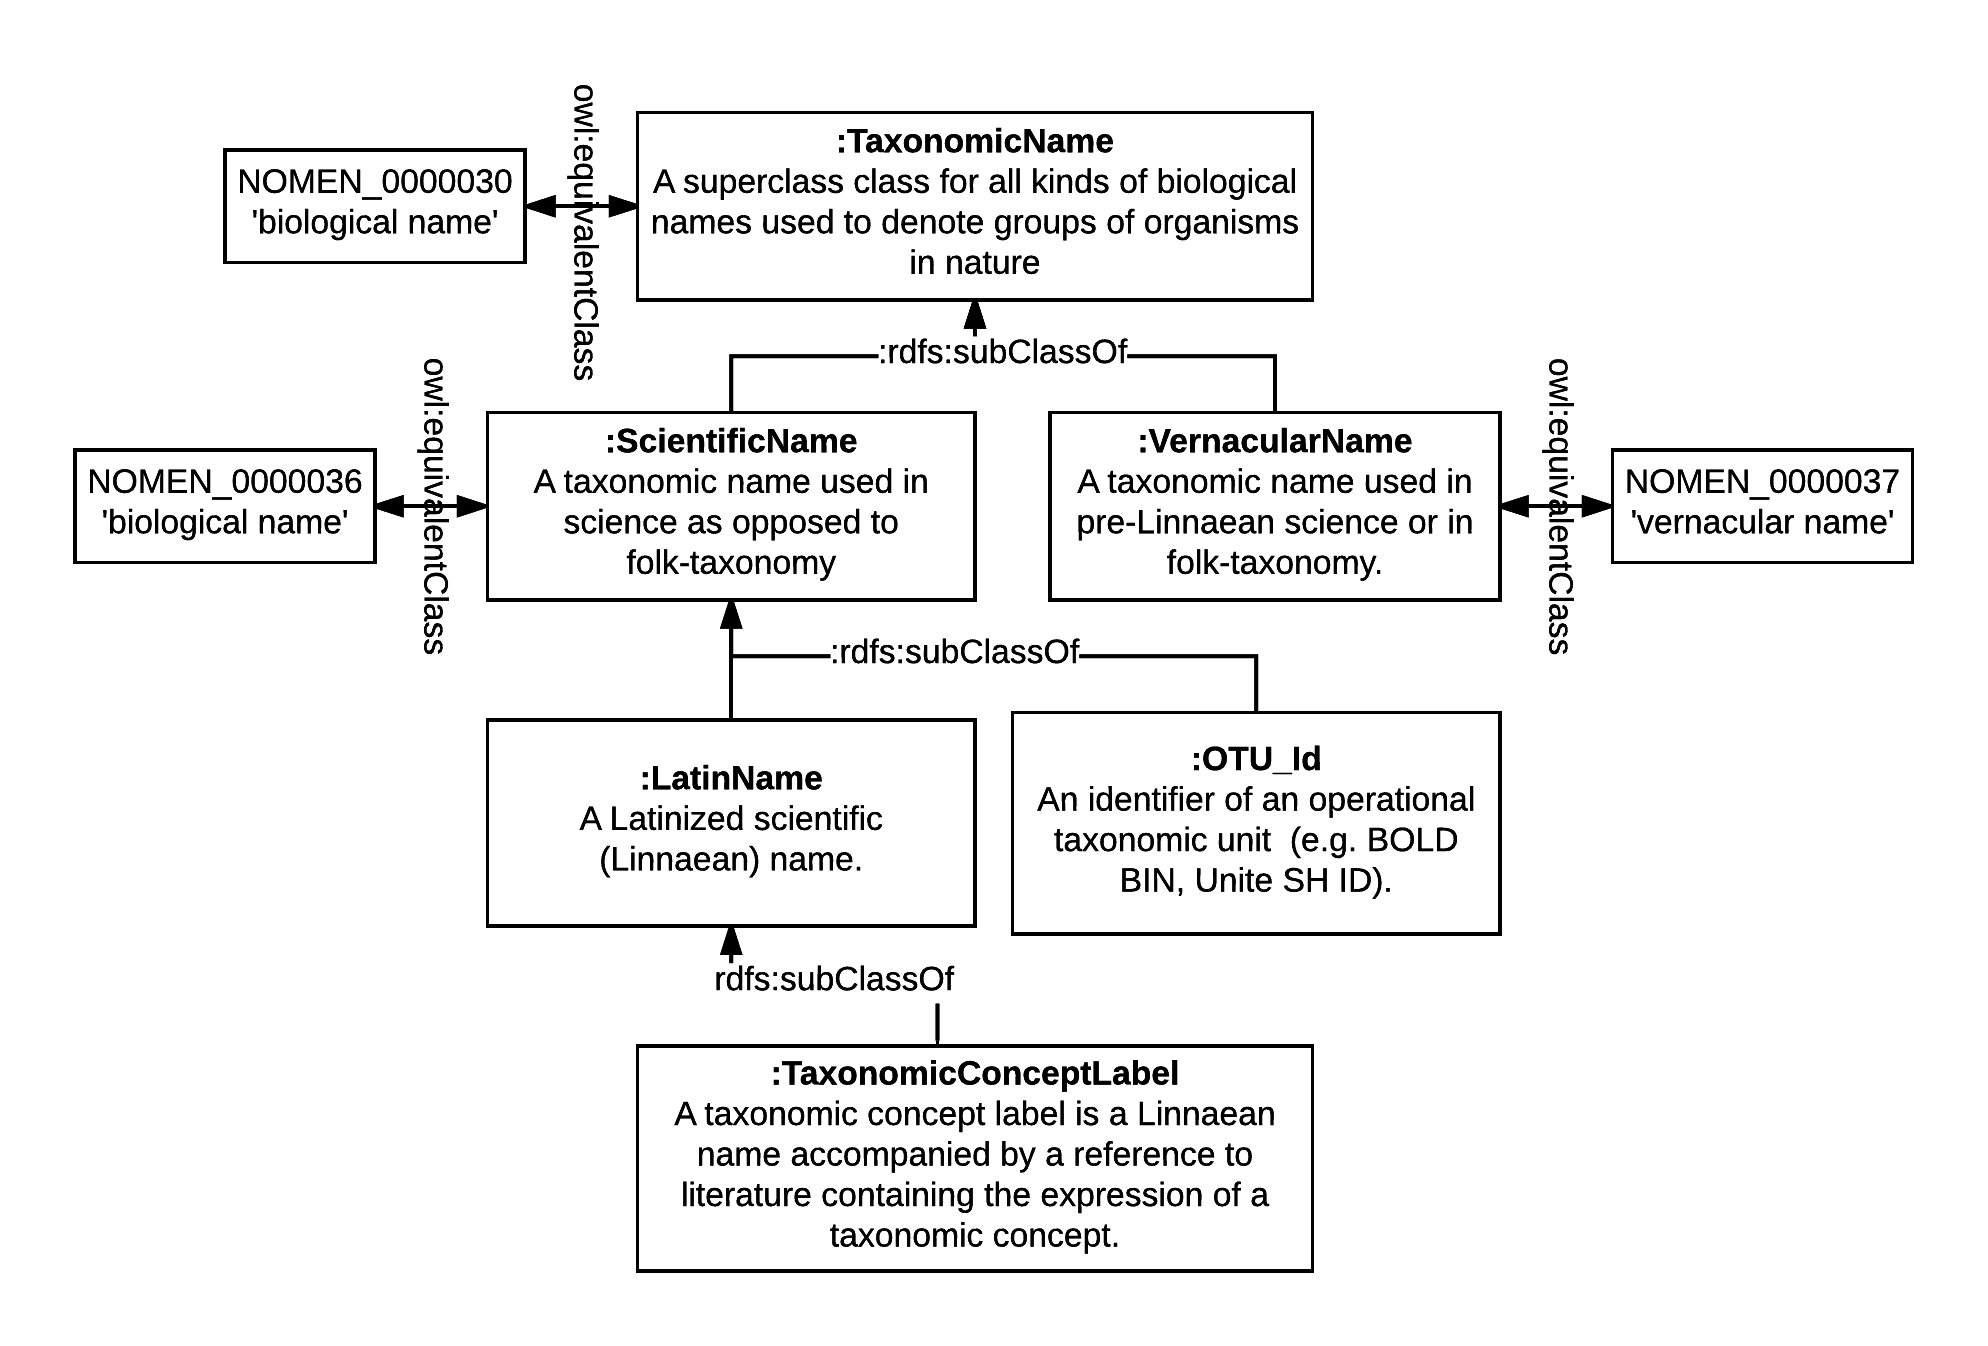
\includegraphics[width=\textwidth]{Figures/taxonomic-name-class-hierarchy-diagram}
  \decoRule
  \caption[Taxonomic name class hierarchy diagram.]{We created this class hierarchy to accommodate both traditional taxonomic name usages and the usage of taxonomic concept labels and operational taxonomic units.}
  \label{taxonomic-name-class-hierarchy-diagram}
\end{figure}

For example, ``\emph{Heser stoevi} Deltschev 2016, sp. n.'' is a taxonomic name usage. The cursive text followed by the author and year of the original species description is the latinized scientific name. The abbreviation ``sp. n.'' stands for the Latin \emph{species novum}, indicating the discovery of a new taxon.

We also introduce the class Taxonomic Concept Label ({\tt :TaxonomicConceptLabel}). A taxonomic concept label (TCL) is a Linnaean name plus a reference to a publication, where the discussed taxon is circumscribed. The link is via the keyword ``sec.'' (Latin for (\emph{secundum}, \cite{berendsohn_concept_1995}). An example would be "\emph{Andropogon virginicus} var. \emph{tenuispatheus} sec. \cite{blomquist_grasses_1948}". Here, \cite{blomquist_grasses_1948} is a valid bibliographic reference to the publication where the concept is circumscribed.

We extracted taxonomic status abbreviations from about 4,000 articles across four taxonomic journals (ZooKeys, Biodiversity Data Journal, PhytoKeys, and MycoKeys) in order to create a taxonomic status vocabulary (see appendices) that covers the eight most common cases (Table \ref{taxonomic-status-vocabulary}). The Latin abbreviations that have been classified into these classes can be found on the OpenBiodiv-O GitHub page. (See Methods for more details).

\begin{table}[h!]
\caption{OpenBiodiv Taxonomic Status Vocabulary.}
\begin{tabular}{ccc}
\hline
Vocabulary Instance QName & Example Abbrev & Comment\\ \hline
{\tt :TaxonomicUncertainty} & \emph{incertae sedis} & Taxonomic Uncertainty\\
{\tt :TaxonDiscovery} & \emph{sp. n.} & Taxonomic Discovery \\
{\tt :ReplacementName} & \emph{comb. n.} & Replacement Name \\
{\tt :UnavailableName} & \emph{nomen dubium} &  Unavailable Name \\
{\tt :AvailableName} & \emph{stat. rev.} & Available Name \\
{\tt :TypeSpecimenDesignation} & \emph{lectotype designation} & Type Specimen Designation \\
{\tt :TypeSpeciesDesignation} & \emph{type species} & Type Species Designation\\
{\tt :NewOccurrenceRecord} & \emph{new country record} & New Occurrence Record (for region)\\
\hline
\end{tabular}
\label{taxonomic-status-vocabulary}
\end{table}

Based on our analysis of taxonomic statuses, we have identified two Code-compliant patterns of relationship between latinized scientific names (Fig. \ref{scientific-name-patterns}). The pattern \emph{replacement name}, implemented via the property {\tt :replacementName}, indicates that a certain Linnaean name should be used instead of another Linnaean name. It covers a wide variety of cases in the Codes, such as, for example, the placement of one species taxon in a new genus ("comb. n."), the correction of a name for nomenclatural reasons ("nomen novum"), or the application of the Principle of Priority for the discovery of synonyms ("syn. nov.", \cite{international_commission_on_zoological_nomenclature_official_2017}).

\begin{figure}[h!]
 \centering
  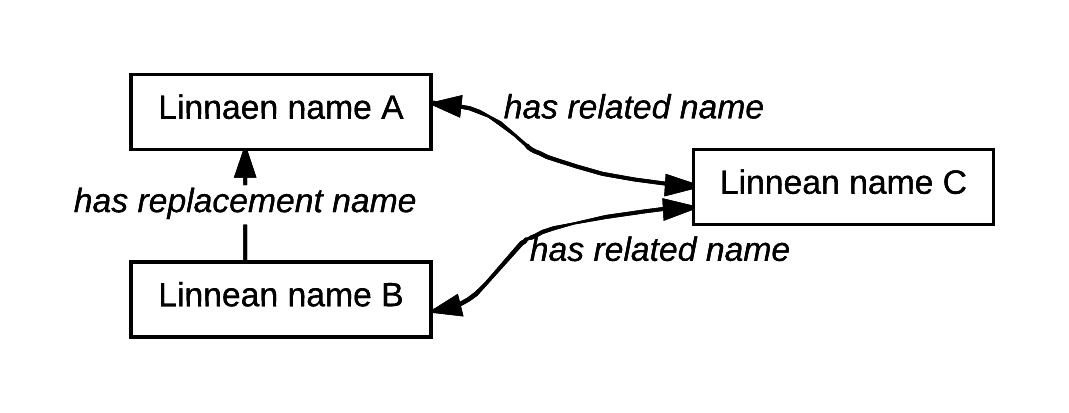
\includegraphics[width=\textwidth]{Figures/scientific-name-patterns}
  \decoRule
  \caption[Scientific name patterns diagram.]{
  Chains of \emph{replacement names} can be followed to find the currently used name. \emph{Related name} indicates that two names are related somehow, but not which one is preferable.}
  \label{scientific-name-patterns}
\end{figure}

The other pattern is that of \emph{related names} ({\tt :relatedName}). It is a broader pattern, indicating that two names are somehow related. For example, they may be synonyms, with one replacing the other, or they may point to taxonomically related taxonomic concepts. For example, \emph{Harmonia manillana} (\cite{mulsant_monographie_1866}) is related to \emph{Caria manillana} \cite{mulsant_monographie_1866} since, as per \cite{poorani_harmonia_2016}, a name-bearing type (lectotype) of \emph{Harmonia manillana} (\cite{mulsant_monographie_1866}) sec. Poorani \cite{poorani_harmonia_2016} is named \emph{Caria manillana} \cite{mulsant_monographie_1866}.

\subsubsection*{Semantics, alignment and usage}
As evident from Fig.~\ref{taxonomic-name-class-hierarchy-diagram}, OpenBiodiv-O taxonomic names are aligned to NOMEN names.

The linking between text and taxonomic names must pass through the intermediary class Taxonomic Name Usage. As parts of the manuscript, taxonomic name usages link document components to taxonomic names. Taxonomic name usages are \emph{contained} in sections such as Treatment, and \emph{mention} a taxonomic name as illustrated in the example in Fig. \ref{example-taxonomic-name-usage}.

\begin{figure}[h!]
\centering
  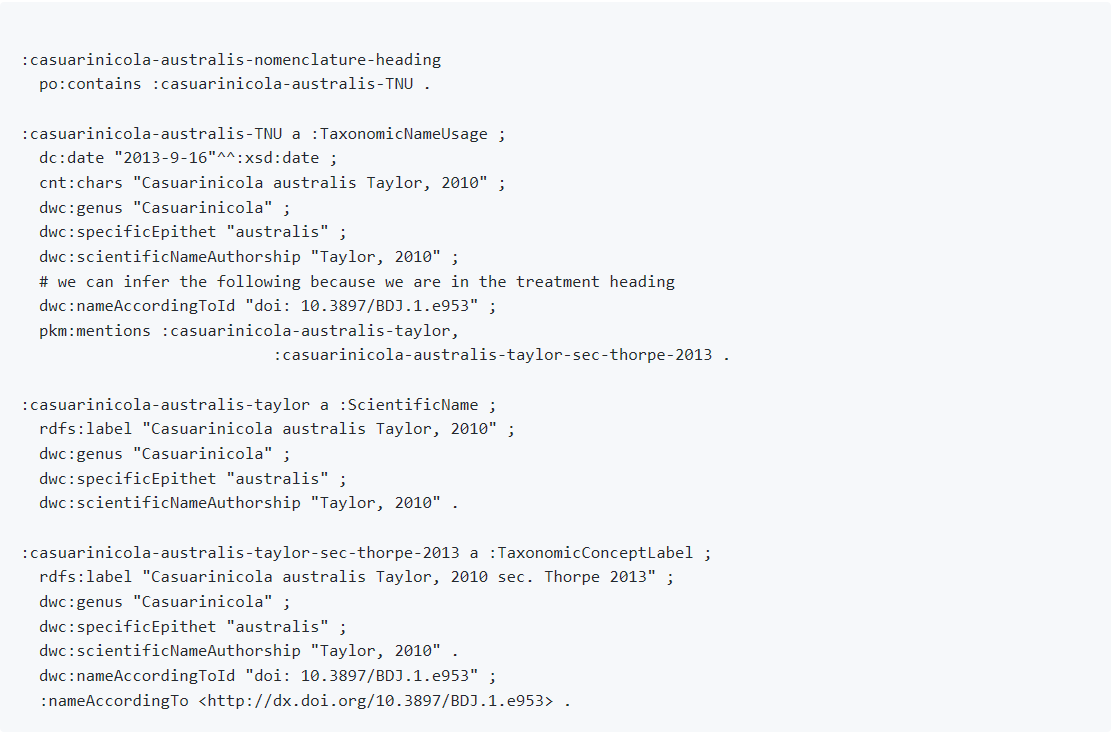
\includegraphics[width=\textwidth]{Figures/example-taxonomic-name-usage}
  \decoRule
  \caption[Example taxonomic name usage.]{
  This examples shows how taxonomic name usages link document components to taxonomic names. The code is in Turtle.}
  \label{example-taxonomic-name-usage}
\end{figure}

\subsection{Semantic Modeling of the Taxonomic Concepts}

In OpenBiodiv-O taxonomic names are not the carriers of semantic information about taxa. This task is accomplished by a new class, Taxonomic Concept ({\tt :TaxonomicConcept}). A taxonomic concept is the theory that a taxonomist forms about a taxon in a scholarly biological taxonomic publication and thus always has a taxonomic concept label. We also introduce a more general class, Operational Taxonomic Unit ({\tt :OperationalTaxonomicUnit}) that can be used for all kinds of taxonomic hypotheses, including ones that don't have a proper taxonomic concept label. The class hierarchy has been illustrated in Fig.~\ref{taxonomic-concept-diagram}.

\begin{figure}[h!]
\centering
  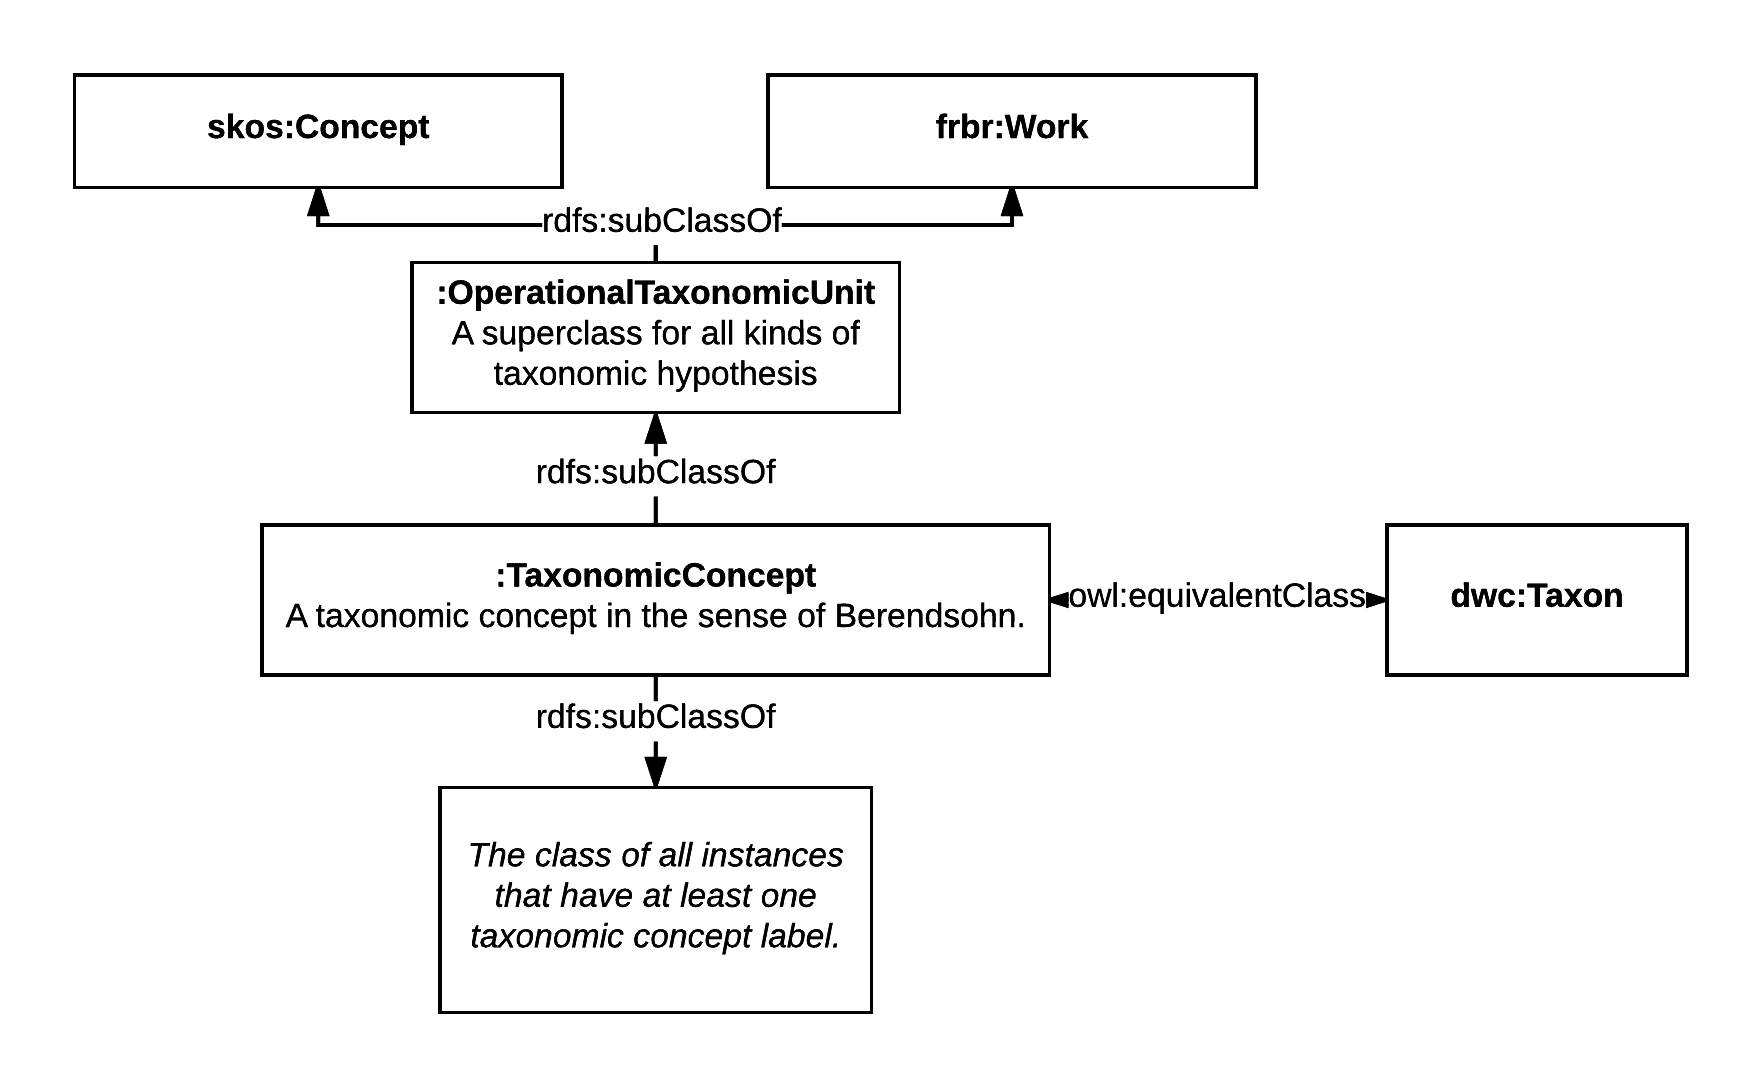
\includegraphics[width=\textwidth]{Figures/taxonomic-concept-diagram}
  \decoRule
  \caption[Taxonomic concept diagram.]{
  A taxonomic concept is a {\tt skos:Concept}, a {\tt frbr:Work}, a {\tt dwc:Taxon} and has at least one taxonomic concept label.}
  \label{taxonomic-concept-diagram}
\end{figure}

Taxonomic concepts are related to taxonomic names---including taxonomic concept labels---via the property \emph{has taxonomic name} ({\tt :taxonomicName}) and its sub-properties mimicking in their range the hierarchy of taxonomic names that we introduced earlier. We have defined a property specifically to link taxonomic concepts to taxonomic concept labels, \emph{has taxonomic concept label} ({\tt :taxonomicConceptLabel}). The property hierarchy diagram is shown in Fig.~\ref{name-property-hierarchy}.

\begin{figure}[h!]
\centering
  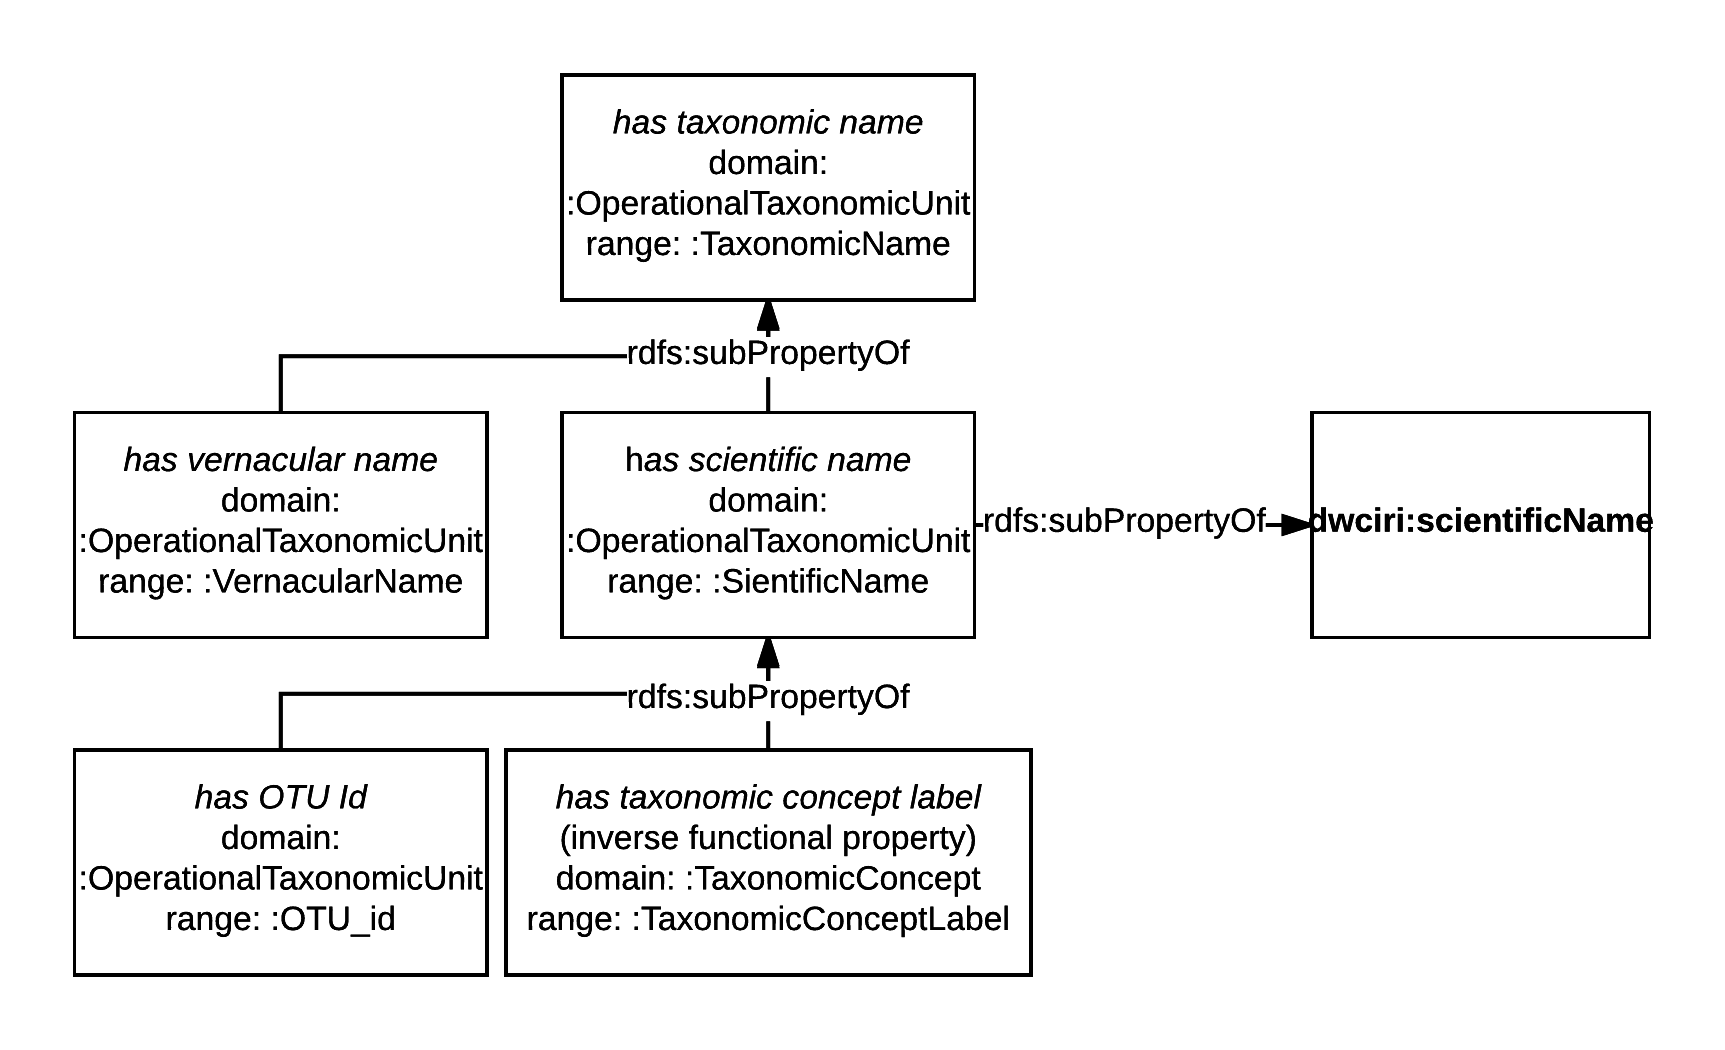
\includegraphics[width=\textwidth]{Figures/name-property-hierarchy}
  \decoRule
  \caption[axonomic name property hierarchy diagram.]
  {Property hierarchy is aligned with the taxonomic name class hierarchy and with DarwinCore.}
  \label{name-property-hierarchy}
\end{figure}

There are two ways to relate taxonomic concepts to each other (Fig. \ref{taxonomic-concept-relationships-diagram}). As we pointed out earlier, historically taxonomic concepts form the hierarchy known as biological taxonomy. To express such simple semantic relations, it is fully sufficient to use the SKOS semantic vocabulary \cite{miles_skos_nodate}. 

\begin{figure}[h!]
\centering
  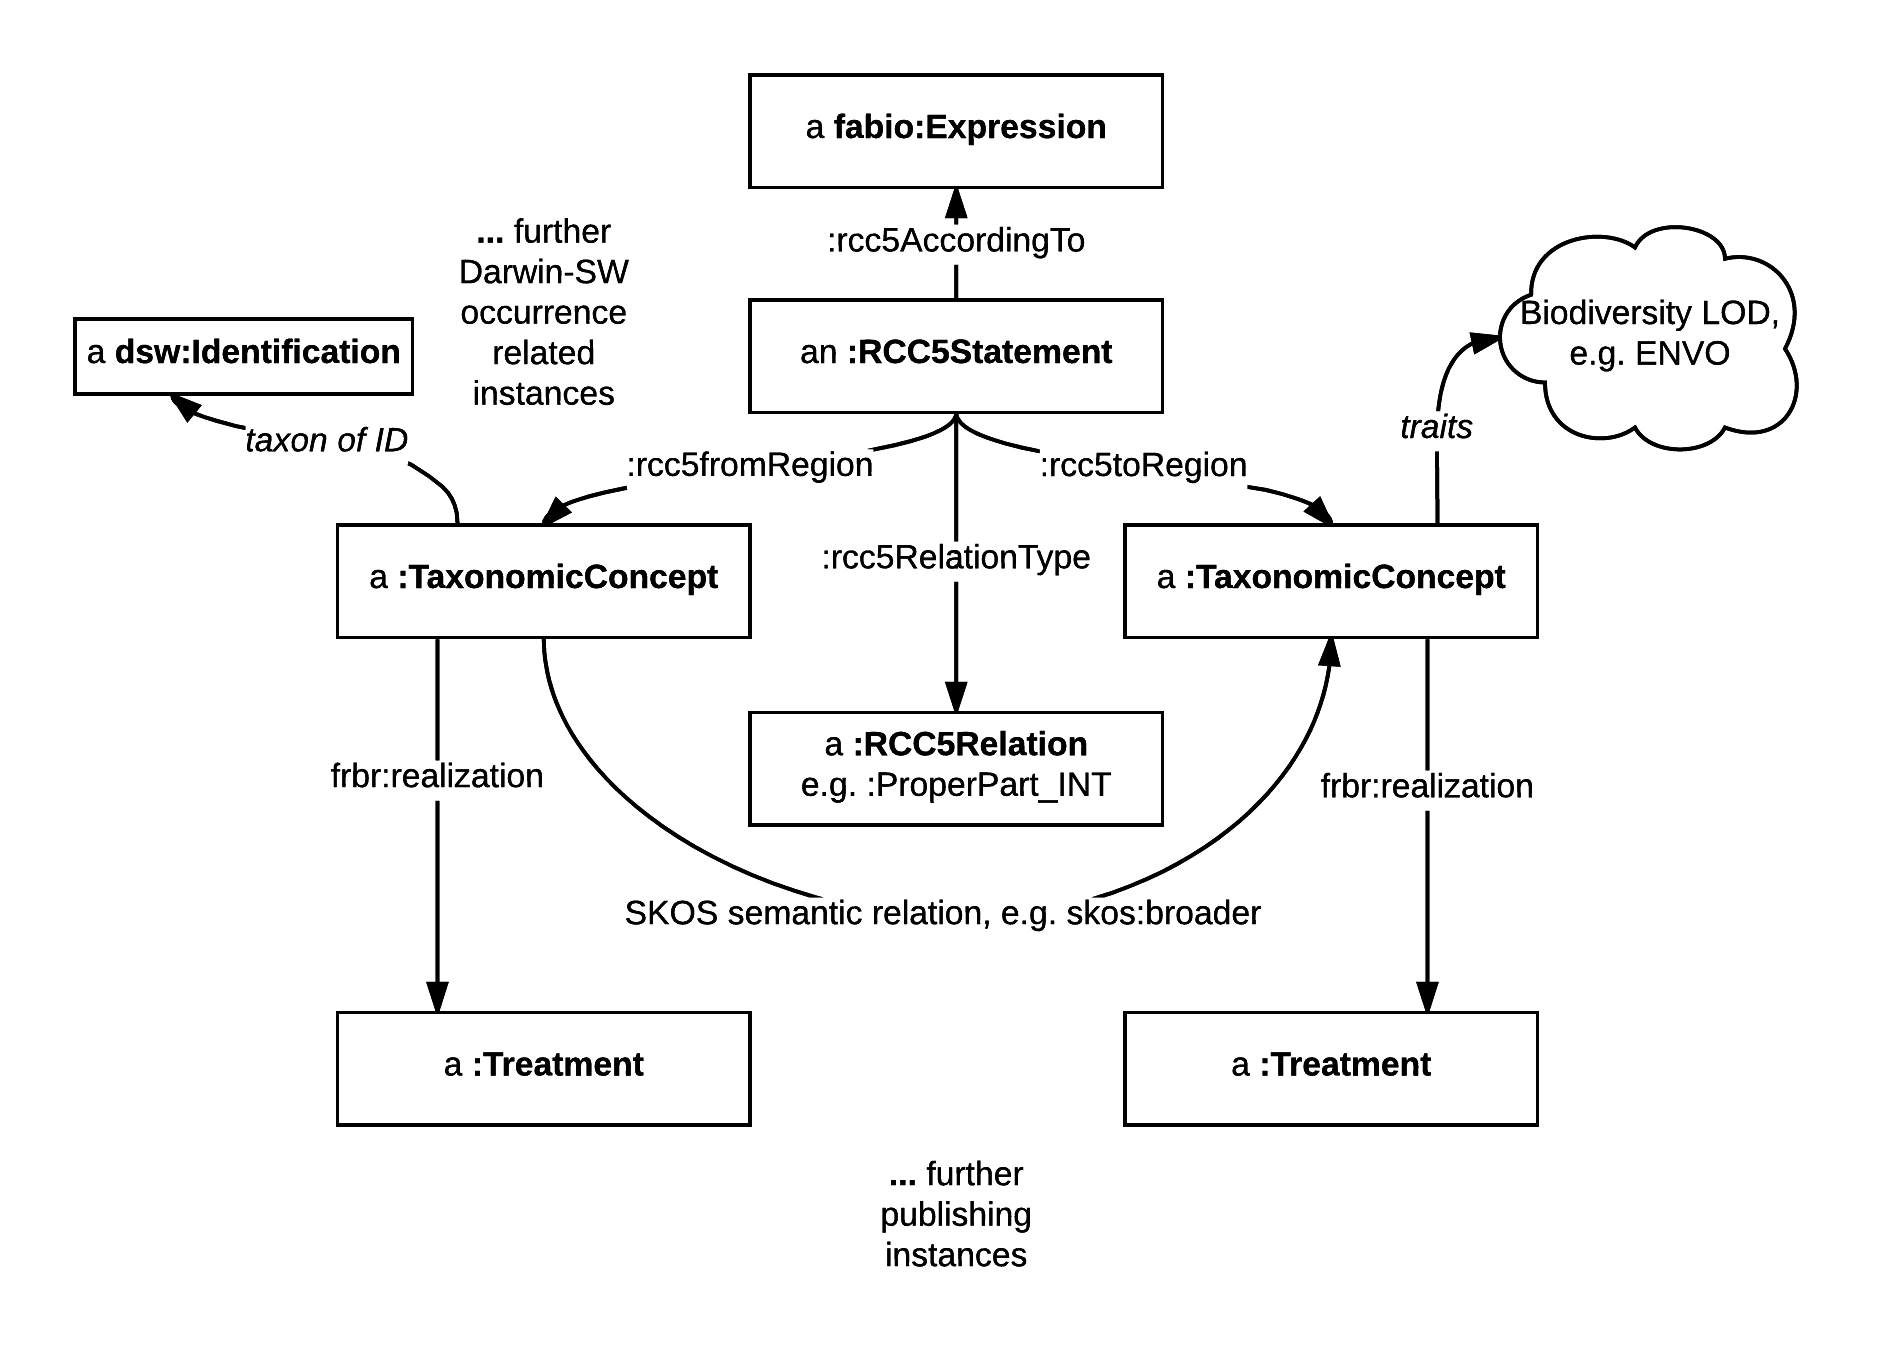
\includegraphics[width=\textwidth]{Figures/taxonomic-concept-relationships-diagram}
  \decoRule
  \caption[Taxonomic concept relationships diagram.]{In order to express an RCC-5 relationship between concepts, create an {\tt :RCC5Sgtatement} and use the corresponding properties to link two taxonomic concepts via it. Further, taxonomic concepts are linked to traits (e.g. ecology in ENVO), occurrences (e.g. Darwin-SW) and realize treatments.}
  \label{taxonomic-concept-relationships-diagram}
\end{figure}

However, these simple relationships are not well suited for machine reasoning. This is why Franz and Peet \cite{franz_perspectives:_2009} suggested, building on previous work by e.g. \cite{koperski_referenzliste_2000}, to use the RCC-5 language to express relationships between taxonomic concepts. Furthermore, the Euler (\cite{chen_euler/x:_2014}) program was developed, which uses Answer Set Programming (ASP) to reason over RCC-5 taxonomic relationships. An answer set reasoner is not part of  OpenBiodiv as this task can be accomplished by Euler; however, we have provided an RCC-5 dictionary class ({\tt :RCC5Dictionary}), an RCC-5 relation term class ({\tt :RCC5Relation}), a vocabulary of such terms to express the RCC-5 relationships in RDF (see appendices), as well as a class and properties to express RCC-5 statements ({\tt :RCC5Statement}, {\tt :rcc5Property}, and subproperties). 

\subsubsection{Semantics and alignment}

We introduce Taxonomic Concept as equivalent ({\tt owl:equivalentClass}) to the DwC term Taxon ({\tt dwc:Taxon}) \cite{noauthor_darwincore_nodate}. However, by including "concept" in the class' name, we highlight the fact that the semantics it carries reflect the scientific theory of a given author about a taxon in nature. As we mentioned earlier, our ontology models the ongoing still unfinished process of taxonomic discovery. For this reason, we also derive Taxonomic Concept from Work. This derivation fits the definition of Work in FRBR/FaBiO, which is \emph{"a distinct intellectual or artistic creation."} Finally, as we use SKOS to connect taxonomic concepts to each other, we derive Taxonomic Concept from SKOS Concept.

As with other semantic publishing-related aspects of the ontology, the creation of the RCC-5 vocabulary follows the SPAR Ontologies' model. Thus OpenBiodiv RCC-5 Vocabulary ({\tt :RCC5RelationshipTerms}) is a SKOS concept scheme and every RCC-5 Relation is a SKOS concept. This allows to seamlessly share this vocabulary with other publishers of biodiversity information that also follow the SPAR Ontologies' model.

It is important to note that we have aligned the subproperty of \emph{has taxonomic name}, \emph{has scientific name} ({\tt :scientificName}), to the DwC property {\tt dwciri:scientificName}. The difference is that while the DwC property is unbound and provides more flexibility, the \mbox{OpenBiodiv-O} property has the domain Taxonomic Concept and the range Scientific Name and provides for inference. Furthermore, \emph{has taxonomic concept label} is an inverse-functional property with the domain Taxonomic Concept. This means that a given taxonomic concept label uniquely determines its taxonomic concept. This is accomplished by a minimum cardinality restriction on the property.

Together with the declaration of \emph{has taxonomic concept label} to be an inverse functional property, we can now list what types of relationships between names and taxonomic concepts are allowed: (1) The relationship between a taxonomic concept and a name that is not a taxonomic concept label is many-to-many---i.e. one Linnaean name can be a mention of multiple taxonomic concepts, and one taxonomic concept may have multiple Linnaean names. (2) The relationship between a taxonomic concept and a taxonomic concept label is one-to-many: while a taxonomic concept may have more than one (at least one is needed) labels, every label uniquely identifies a concept. These logical restrictions make taxonomic concept labels into unique identifiers to taxonomic concepts, something that Linnaean names are not.

\subsubsection{Usage} For an example of linking two taxonomic concepts to each other, let us look at the species-rank concept \emph{Casuarinicola australis} \cite{taylor_casuarinicola_2010} sec. \cite{thorpe_casuarinicola_2013}. It is a narrower concept than the genus-rank concept of \emph{Casuarinicola} \cite{taylor_casuarinicola_2010} sec. \cite{taylor_casuarinicola_2010}. As we have aligned our concepts to SKOS, we can use its vocabulary to express this statement as seen in the example in Fig. \ref{example-simple-taxonomic-concept-relationships}. A further example of how to utilize the OpenBiodiv RCC-5 vocabulary is found in Fig.~\ref{example-rcc5-taxonomic-concept-relationships}.

\begin{figure}[h!]
\centering
  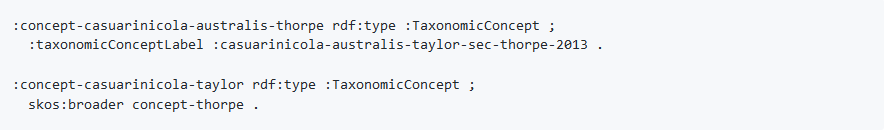
\includegraphics[width=\textwidth]{Figures/example-simple-taxonomic-concept-relationships}
  \decoRule
  \caption[Example simple taxonomic concept relationships.]
  {We can use SKOS semantic properties to illustrate simple relationships between taxonomic concepts.}
  \label{example-simple-taxonomic-concept-relationships}
\end{figure}

\begin{figure}[h!]
\centering
  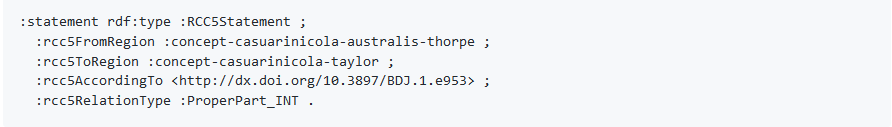
\includegraphics[width=\textwidth]{Figures/example-rcc5-taxonomic-concept-relationships}
  \decoRule
  \caption[Example of RCC-5 taxonomic concept relationships.]{In order to express an RCC-5 relationship between concepts, create an {\tt :RCC5Sgtatement} and use the corresponding properties to link two taxonomic concepts via it. SKOS relations relate concepts directly.}
  \label{example-rcc5-taxonomic-concept-relationships}
\end{figure}

Furthermore, thanks to the alignment to DwC, we treat instances of our class Taxonomic Concept as functionally equivalent to DwC Taxa. This makes linking to other biodiversity ontologies possible. For example, the Open Biomedical Ontologies' (OBO) Population and Community Ontology (PCO, \cite{walls_semantics_2014}) has a class "collection of organisms" (\url{http://purl.obolibrary.org/obo/PCO_000000}) that can be considered a superclass of DwC Taxon. Therefore, every taxonomic concept is a collection of organisms and the application of OBO properties on it is allowed.

In the paper that inspired our \emph{Casuarinicola} example (\cite{thorpe_casuarinicola_2013}), we read: \emph{"On 26 February 2013, the species was found to be fairly common on Casuarina trees at Thomas Bloodworth Park, Auckland."} This statement can be interpreted (in ENVO) as meaning that the taxonomic concept that the author formulated implies that it includes the habitat "forest biome" (\url{http://purl.obolibrary.org/obo/RO_0002303}). The RDF example is shown in Fig.~\ref{example-envo}.

\begin{figure}[h!]
\centering
  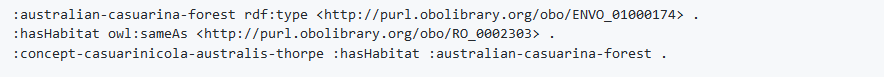
\includegraphics[width=\textwidth]{Figures/example-envo}
  \decoRule
  \caption[Example of combining ENVO with OpenBiodiv-O.]{We create a shortcut for \emph{has habitat} and instance of the "forest biome" and link them to our taxonomic concept in order to express the fact that specimens of it have been found to live in \emph{Casuarina} trees.}
  \label{example-envo}
\end{figure}

As we pointed out earlier, taxonomic concepts have an intensional component (traits or characters) and an ostensive component (a list of occurrences belonging to the concept). The ostensive component can be expressed by linking occurrences to the taxonomic concepts via Darwin-SW. This is possible as we have aligned the Taxon Concept class to DwC Taxon used by Darwin-SW. For an example refer to \cite{baskauf_darwin-sw:_2016}.

Lastly, describing traits is an active area of ontological research (\cite{huang_oto:_2015}). Due to the very complex language used to describe morphological characteristics, the Ontology Term Organizer (OTO, \cite{huang_oto:_2015}) software was developed to allow for user-created vocabularies. An avenue for a follow-up project is to work with OTU to express traits and trait equivalences (in the taxonomic sense) during the population of OpenBiodiv with triples (\cite{hong_explorer_2018}).

Last, the interpretation of Taxonomic Concepts as Work means that they are realized by taxonomic treatments (e.g. Fig~\ref{example-treatment-concept}).

\begin{figure}[h!]
\centering
  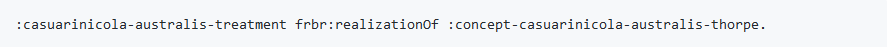
\includegraphics[width=\textwidth]{Figures/example-treatment-concept}
  \decoRule
  \caption[Example connection between a treatment and a taxonomic concept.]{A treatment is the realization of a taxonomic concept.}
  \label{example-treatment-concept}
\end{figure}

\section{Discussion}

OpenBiodiv-O is---together with the Treatment Ontologies \cite{catapano_treatment_2016}---the first effort to model taxonomic articles as RDF. It introduces classes and properties in the domains of biodiversity publishing and biological taxonomy and aligns them with the SPAR Ontologies, the Treatment Ontologies, the Open Biomedical Ontologies (OBO), TaxPub, NOMEN, and DarwinCore. We believe this introduction bridges the ontological gap that we had outlined in our aims and allows for the creation of a Linked Open Dataset (LOD) of biodiversity information (biodiversity knowledge graph, \cite{senderov_open_2016, page_towards_2016}).

Furthermore, this biodiversity knowledge graph, together with this ontology, additional semantic rules, and user software will form the OpenBiodiv Knowledge Management System. This system, as any taxonomic information system should, has taxonomic names as a key building block. For any given taxonomic name, the user will be able to rely on two patterns---\emph{replacement name} and \emph{related name}---to get answers to two questions of high importance to the working taxonomist. First: what is the current and historical usage of any given Linnaean name? Second: given a particular name, what other related names ought to be considered in a taxonomic discussion?

Both may be useful in building semantic search applications and the latter, in particular, is actively being researched by a group at the National Center for Text Mining in the UK (NaCTeM, \cite{nguyen_constructing_2017}). \mbox{OpenBiodiv-O} proper does not include a mechanism for inferring replacement names and related names; however, such mechanisms are part of the OpenBiodiv knowledge system via SPARQL rules using information encoded in the document structure (Nomenclature section). Another way to infer related names is via a machine learning approach to obtain feature vectors of taxonomic names.  Note that the ontology can describe related names independent of the process of their generation and will enable the comparison of both approaches in a future work.

On the other hand, by using \mbox{OpenBiodiv-O}, a knowledge-based system does not have to have a backbone name-based taxonomy. A backbone taxonomy is a single, monolithic hierarchy in which any and all conflicts or ambiguities have been pragmatically (socially, algorithmically) resolved, even if there is no clear consensus in the greater taxonomic domain. Such backbone taxonomies are used in systems that rely solely on taxonomic names (and not concepts) as bearers of information. They are needed as it is impossible, in such a system, to express two different sets of statements for a single name.

In OpenBiodiv, however, multiple hierarchies of taxonomic concepts may exist. For example, large synthetic taxonomies such as GBIF's backbone taxonomy (\cite{gbif_secretariat_gbif_2017}) or Catalogue of Life\footnote{\href{http://www.catalogueoflife.org/}{http://www.catalogueoflife.org/}} may not agree or may have some issues \cite{page_gbif_2012}. With OpenBiodiv-O, we may, in fact, incorporate both these taxonomies at the same time! It is possible according to the ontology to have two sets of taxonomic concepts (even with the same taxonomic names) with a different hierarchical arrangement. By allowing this, we leave some room for human interpretation as an additional architectural layer. Thus, we delay the decision of which hierarchy to use to the user of the system (e.g. a practicing taxonomist) and not to the system's architect. Due to this design feature, it is likely that our system stands a better chance to be trusted as a science process-enabling platform as the system architects don't force a taxonomic opinion on the practicing taxonomist.

It should be noted that a successful concept-based system exists for the taxonomic order Aves (birds, \cite{lepage_avibase_2014}). The main issue that we will face is to develop tools to enable expert users to annotate taxonomic concepts with the proper relationships as only recently individual articles utilizing concept taxonomy in addition to nomenclature have been published (\cite{franz_two_2016,jansen_phylogenetic_2015,franz_three_2017}). We do believe that their numbers will rise driven by the realization that there are some problems with relying solely on Linnaean names for the identification of taxonomic concepts (\cite{patterson_names_2010,remsen_use_2016, franz_names_2016}). Concept taxonomy may, in fact, become even more important in the future as conservation efforts face challenges due to unresolved taxonomies (\cite{garnett_taxonomy_2017}). Properly aligning taxonomic concepts to nomenclature across revisions (\cite{franz_logic_2016-1}) may be the solution.

Together with taxonomic information, the ontology allows modeling the source information in a knowledge base. This will be useful for meta-studies, for the purposes of reproducible research, and other scholarly purposes. Moreover, it will be an expert system as the knowledge extracted will come from scholarly publications. We envision the system to be able to address a wide variety of taxonomic competency questions raised by researchers (\cite{pro-ibiosphere_competency_2013}). Examples include: "Is X a valid taxonomic name (in a nomenclatorial sense)?" ``Which treatments use different names for the same taxon concepts?'' ``Which treatments are nomenclatorially linked (including homonyms!) to another treatment?''

In the next Chapter we will show how we populated the ontology with triples extracted from Pensoft journals, legacy journals text-mined by Plazi, as well as databases such as GBIF's taxonomic backbone (\cite{gbif_secretariat_gbif_2017}). Special effort will be made to link the dataset to the Linked Open Data cloud via resources such as geographic or institution names. In terms of extending the ontological model, more research needs to go into modeling the taxonomic concept circumscription---creating ontologies for morphological, genomic, or ecological traits. 

\section{Conclusions}

The chapter provides an informal conceptualization of the taxonomic process and a formalization in OpenBiodiv-O. It introduces classes and properties in the domains of biodiversity publishing and biological systematics and aligns them with the important domain-specific ontologies. By bridging the ontological gap between the publishing and the biodiversity domains, it will enable the creation of Open Biodiversity Knowledge Management System, consisting of (1) the ontology itself; (2) a Linked Open Dataset (LOD) of biodiversity information (biodiversity knowledge graph); and (3) user interface components aimed at searching, browsing and discovering knowledge in big corpora of previously dispersed scholarly publications. Through the usage of taxonomic concepts, we have included mechanisms for democratization of the scholarly process and not forcing a taxonomic opinion on the users.
\chapter{OpenBiodiv Linked Open Dataset}
\label{chapter-lod}

We have created a Linked Open Dataset, OpenBiodiv LOD, comprising biodiversity information extracted from Pensoft journals and Plazi Treatment Bank and which was integrated with the GBIF Taxonomic Backbone. As ontology, we use the new \mbox{OpenBiodiv-O} developed by us. We propose to the biodiversity informatics community to use OpenBiodiv LOD as the central point for a biodiversity knowledge graph! OpenBiodiv LOD is an RDF dataset adhering to the principles of Linked Open Data. It is available under \url{http://graph.openbiodiv.net}, which provides a SPARQL endpoint for it.

OpenBiodiv LOD is a synthetic dataset. It does not contain previously unpublished data. Instead it integrates information previously found in academic journals and databases into one dataset. It also contains  extracted, previously unaccessible information from the original datasets in the form of relations. In the next few paragraphs we discuss the sources of information that were combined to from OpenBiodiv LOD and the types of resources that have been extracted, as well as the overall data model. We also discuss the principles of Linked Open Data that tie everything together. The chapter ends with many examples of queries on the dataset and with a technical discussion of how it was generated.

\section{Data Sources}

The data in OpenBiodiv at the time of writing this thesis comes from three major sources: the GBIF Backbone Taxonomy (\cite{gbif_secretariat_gbif_2017-1}), journal articles published by Pensoft, and Plazi Treatment Bank (Fig.~\ref{fig:openbiodiv-sources-simple}).

\begin{figure}
\centering
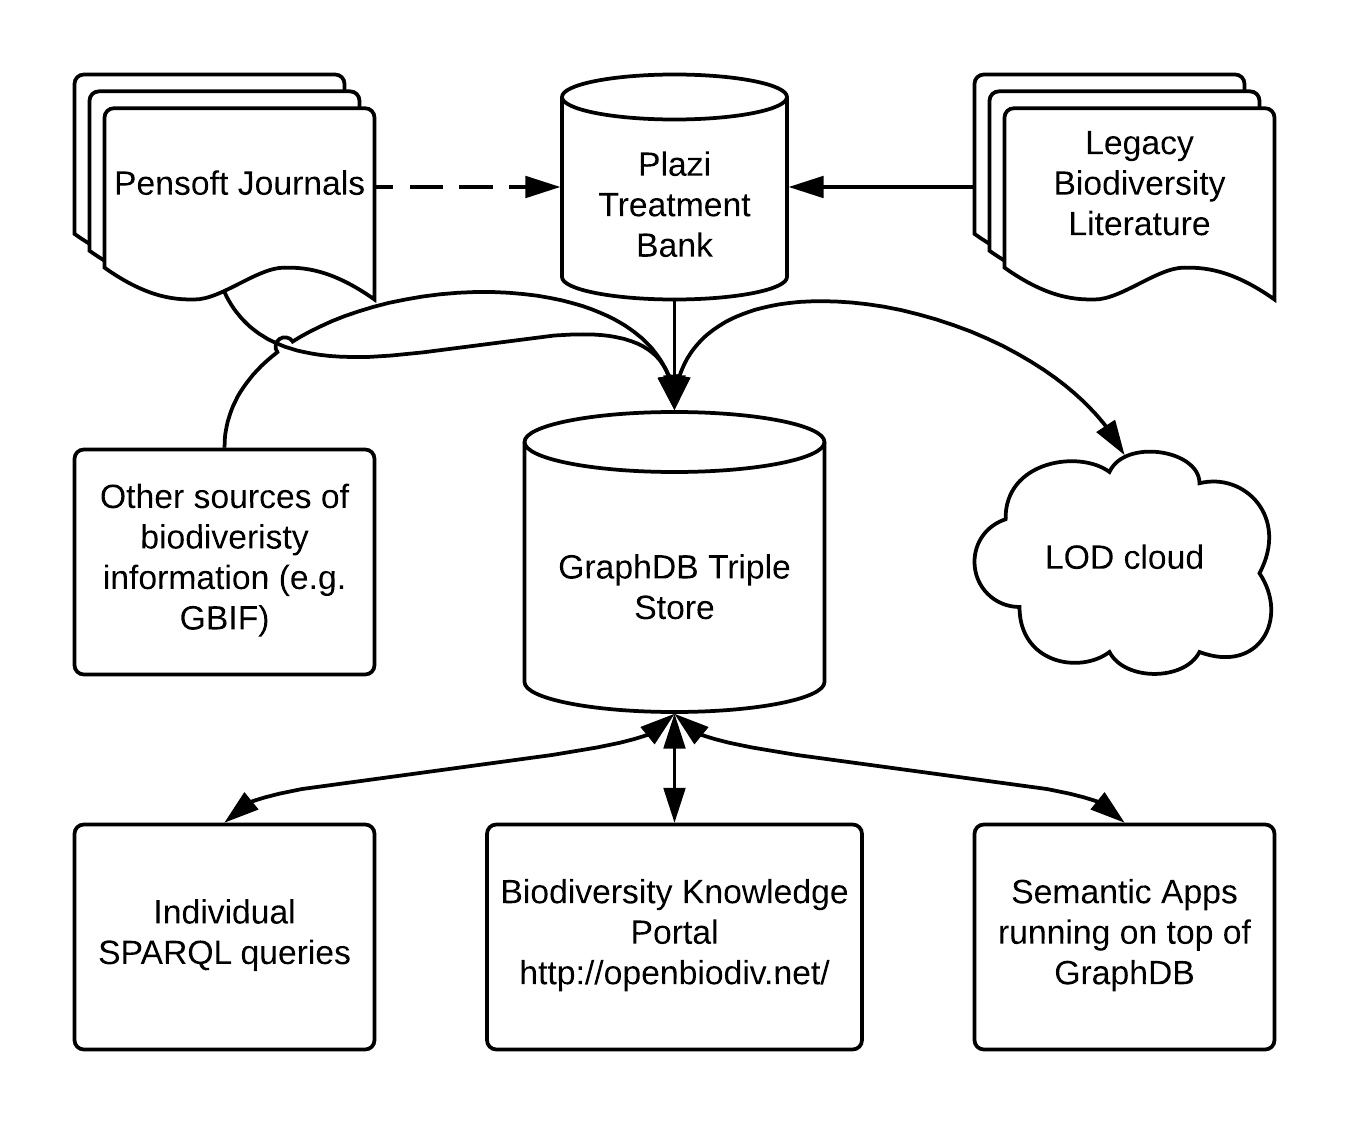
\includegraphics[width=\textwidth]{Figures/openbiodiv-sources-simple}
\decoRule
\caption{A simplified version of the OpenBiodiv architecture presented in Chapter~\ref{chapter-openbiodiv} focusing on the sources of information.}
\label{fig:openbiodiv-sources-simple}
\end{figure}


\subsection{GBIF Backbone Taxonomy}

GBIF is the largest international repository of occurrence data, i.e. data about the presence of an organism of a given taxon at a given place and time. GBIF allows its users to do searches on its occurrence data utilizing a taxonomic hierarchy. For example, it is possible to query the database  for occurrences of organisms belonging to a specific genus: a search for the beetle genus \textit{Harmonia} sec. \cite{gbif_secretariat_gbif_2017-1} on 30 June 2018 returned 575,376 results. This search is possible thanks to the GBIF Backbone Taxonomy also known as Nub (\cite{gbif_secretariat_gbif_2017-1}). Nub is a database organizing taxonomic concepts in a hierarchy covering all names used in occurrence records harvested by GBIF.  It is a single synthetic (algorithmically generated) management classification with the goal of covering all names present in GBIF's datasets. Thus, the GBIF backbone does not represent an expert consensus on how taxa are hierarchically arranged according to evolutionary criteria in Nature.

Keeping in mind this critique, it is evident how the backbone taxonomy allows GBIF to integrate name based information from diverse sources such as Encyclopedia of Life (EOL), Genbank, or the International Union for Conservation of Nature, and provides a facility for taxonomic searching and browsing.

In order to grant the same capabilities to OpenBiodiv, we have imported Nub as instances of {\tt openbiodiv:TaxonomicConcept} according to OpenBiodiv-O. Each GBIF taxonomic concept is linked to an instance of {\tt openbiodiv:ScientificName} and to its parent taxonomic concept via SKOS and RCC-5 (Fig.~\ref{fig:harmonia-halii-visual}). Thus, even though users of OpenBiodiv-LOD have the opportunity of taxonomic search using Nub, we have decoupled scientific names from a single hierarchical representation allowing the future evolution of OpenBiodiv-LOD to incorporate other simultaneous views of taxonomic alignment.

\begin{figure}
\centering
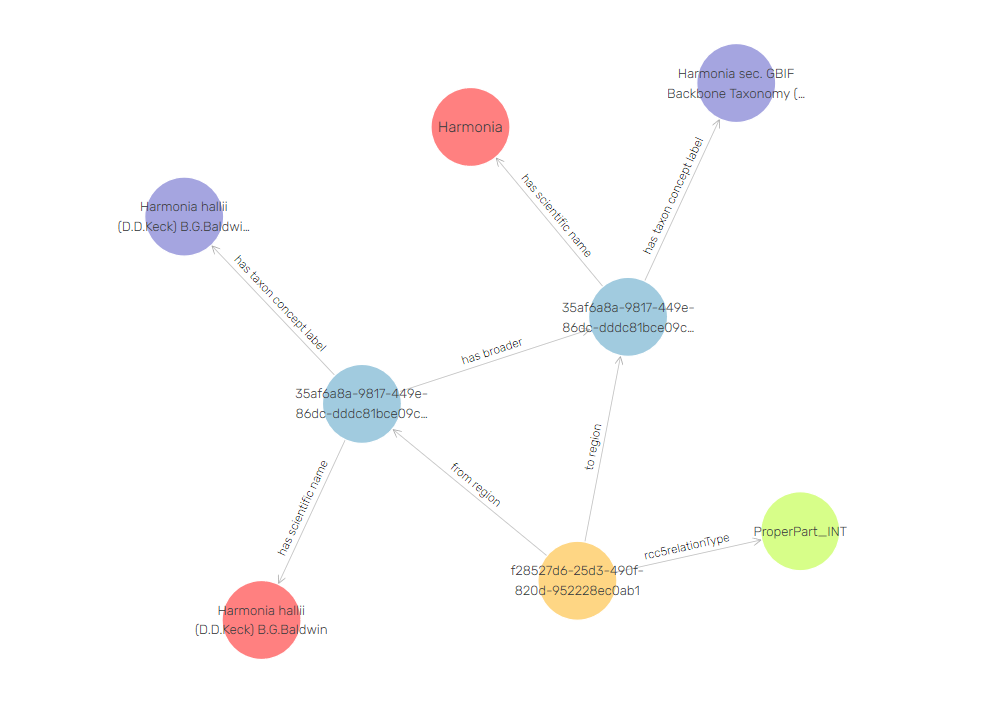
\includegraphics[width=\textwidth]{Figures/harmonia-halii-visgraph}
\decoRule
\caption[Visual graph of \emph{Harmonia halii}]{Illustration of the representation of hierarchical information imported from the GBIF Backbone Taxonomy as two taxonomic concepts, \emph{Harmonia halii} sec. \cite{gbif_secretariat_gbif_2017} and \emph{Harmonia} sec. \cite{gbif_secretariat_gbif_2017}. Each concept has an associated scientific name via \emph{has scientific name}; however, the hierarchical information is not encoded in the names. The hierarchical relationship between \emph{Harmonia halii} sec. \cite{gbif_secretariat_gbif_2017} and \emph{Harmonia} sec. \cite{gbif_secretariat_gbif_2017} is encoded both as SKOS \emph{has broader} and reified via the RCC-5 relationship encoded in {\tt f28527d6-25d3-490f-820d-952228ec0ab1}.}
\label{fig:harmonia-halii-visual}
\end{figure}

Furthermore, as the GBIF backbone taxonomy is updated regularly through an automated process from over 56 sources, future updates may be ingested as different versions into OpenBiodiv-LOD without affecting existing records.

\subsection{Pensoft and Plazi}

All valid articles from the journals published by Pensoft listed in Table~\ref{rdf-pensoft-journals} have been converted to RDF and stored in the biodiversity knowledge graph. Additionally, all valid taxonomic treatments from Plazi Treatment Bank have been converted to RDF and stored in the graph as well. Furthermore, the RDF-ization procedure is triggered automatically on a weekly basis and thus the semantic database is always updated with the newest articles published by Pensoft and newest taxonomic treatments extracted by Plazi. The RDF-ization is made possible by the fact that all Pensoft journals are published as XML according to TaxPub, an extension of the NLM/NCBI journal publishing DTD for taxonomic description (\cite{catapano_taxpub:_2010}) and, similarly, all Plazi treatments follow the TaxonX XML Schema (\cite{penev_xml_2011}). Thus, the RDF-ization pipeline does not require a natural language processing step, as a considerable amount of information is marked-up at the time of publication. We have given an example of how a taxonomic name usage is marked up in a TaxPub article in Listing~\ref{listing:tnu}. The datatypes that have been marked up in TaxPub and TaxonX and whose entities are converted to RDF are listed in Table~\ref{datatypes-taxpub-taxonx}. Note that the marked-up datatypes do not correspond 1-to-1 to the RDF entities that have been created in the graph as TaxPub, TaxonX, and OpenBiodiv-O take slightly different approaches to modeling the biodiversity world. OpenBiodiv-O takes the most granular approach. For example, each taxonomic name usage in a Pensoft article results in a corresponding {\tt openbiodiv:TaxonomicNameUsage} resource and a link to the {\tt openbiodiv:ScientificName} resource that the taxonomic name usage mentions (Fig.~\ref{fig:tnu-vis}).

\begin{lstlisting}[language=XML,
caption=Taxonomic name usage of the name \emph{P. emarginaticeps} in Taxpub. Name parts are tagged with {\tt tp:taxon-name-part} and the expansion of abbreviations (regularization) is marked up with the attribute {\tt reg},
label=listing:tnu, basicstyle=\ttfamily\tiny]
<tp:taxon-name>
  <tp:taxon-name-part taxon-name-part-type="genus" reg="Pristaulacus">
    P.
  </tp:taxon-name-part>
  <tp:taxon-name-part taxon-name-part-type="species" reg="emarginaticeps">
    emarginaticeps
  </tp:taxon-name-part>
  <tp:taxon-name-part taxon-name-part-type="authority">
    Turner 1922
  </tp:taxon-name-part>
</tp:taxon-name> 
\end{lstlisting}

\begin{table}[h!]
\caption{RDF-ized biodiversity journals published by Pensoft.}
      \begin{tabular}{ccc}
        \hline
          Journal Name             & Submission Style & Number of Articles\\  \hline
          ZooKeys                 & Word document & 3829\\
          PhytoKeys               & Word document & 537\\
          MycoKeys                & Word document & 127\\
          Biodiversity Data Journal & Web based (ARPHA) & 490\\
          Journal of Orthoptera Research & Word document & 32
      \end{tabular}
      \label{rdf-pensoft-journals}
\end{table}

\begin{table}[h!]
\caption{Datatypes marked up in TaxPub and TaxonX articles and the corresponding RDF types of the generated RDF resources. The TaxPub and TaxonX columns contain boolean values indicating whether the information about the datatype is retrieved from files encoded in the corresponding schema.}
      \begin{tabular}{cccc}
        \hline
          Datatype             & TaxPub & TaxonX & RDF Type\\  \hline
          Article metadata     & T & T & {\tt fabio:JournalArticle} and related\\
          Keyword group        & T & F & {\tt openbiodiv:KeywordGroup} \\
          Abstract             & T & T & {\tt sro:Abstract}\\
          Title                & T & F & {\tt doco:Title} \\
          Author               & T & T & {\tt foaf:Person} \\
          Introduction section & T & F & {\tt deo:Introduction}\\
          Discussion section   & T & T & {\tt orb:Discussion}\\
          Treatment section    & T & T & {\tt openbiodiv:Treatment}\\
          Nomenclature section & T & T & {\tt openbiodiv:NomenclatureSection}\\
          Materials examined   & T & T & {\tt openbiodiv:MaterialsExamined}\\
          Diagnosis section    & T & T & {\tt openbiodiv:DiagnosisSection} \\
          Distribution section & T & T & {\tt openbiodiv:DistributionSection}\\
          Taxonomic key        & T & T & {\tt openbiodiv:TaxonomicKey}\\
          Figure               & T & T & {\tt doco:Figure}\\
          Taxonomic name usage & T & T & {\tt openbiodiv:TaxonomicNameUsage}
      \end{tabular}
      \label{datatypes-taxpub-taxonx}
\end{table}

\begin{figure}
\centering
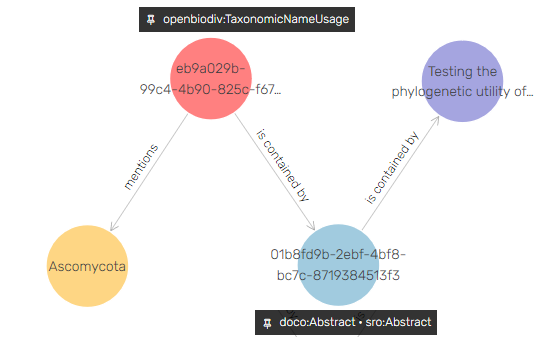
\includegraphics[width=\textwidth]{Figures/tnu-vis}
\decoRule
\caption[Visual graph of a taxonomic name usage]{The taxonomic name usage ({\tt openbiodiv:eb9a029b-99c4-4b90-825c-f670fb88900d}) is linked to the scientific name it mentions, \emph{Ascomycota} and to the part of the article (abstract) that it is contained in.}
\label{fig:tnu-vis}
\end{figure}

\section{Linked Open Data}

Linked Open Data (LOD, \cite{heath_linked_2011}) is a concept of the Semantic Web (\cite{berners-lee_semantic_2001}) applied to ensure that data published on the Web is reusable, discoverable and most importantly to ensure that pieces of data published by different entities can work together. The principles of LOD are the following (\cite{heath_linked_2011})

\begin{enumerate}
\item{Use URIs as names for things.}
\item{Use HTTP URIs so people can lookup these things.}
\item{When someone looks up a URI, provide useful information, using the standards (RDF, SPARQL).}
\item{Include links to other URIs so they can discover more things.}
\end{enumerate}

We have followed these guidelines when creating the OpenBiodiv LOD. We will now discuss each of these points separately.

\subsection{Usage of URIs as resource identifiers}

Every instance in OpenBiodiv LOD is uniquely identifiable by a HTTP URI of the following form: \url{http://openbiodiv.net/uuid-(suffix)}. All instance identifiers in OpenBiodiv LOD follow this schema. The optional suffix field is assigned only to resources extracted from GBIF.

\paragraph{Identfiers for Pensoft and Plazi.} During the RDF-ization of the sources Pensoft and Plazi, when a new concept is discovered (e.g. a person, a scientific name, etc.) a UUID is generated. Then the resource is always referred to in the database by this UUID in the OpenBiodiv namespace, \url{http://openbiodiv.net/}. Pensoft and Plazi furthermore share the UUID part of the identifier in the semi-structured representation of treatments. For example, Lyubomir Penev is a resource identified by \url{http://openbiodiv.net/7a247614-878b-4d01-ab97-bf5fc608dc86}.

\paragraph{Identifiers for GBIF taxonomic concepts.} GBIF offers its taxonomic backbone as a big DarwinCore (\cite{wieczorek_darwin_2012}) tab separated file (TSV). Each row in the TSV corresponds to a taxonomic concept published by GBIF. GBIF does not offer a globally unique ID of its concepts, but only a local ID (e.g. $4239$ is the GBIF ID of concept of Curculionidae sec \cite{gbif_secretariat_gbif_2017}). This is why, we generated a UUID (e.g. for the example \url{35af6a8a-9817-449e-86dc-dddc81bce09c-4239}) for each row of data table published from GBIF. However, each taxonomic concept is linked to a taxonomic name and to a taxonomic concept label (see Chapter~\ref{chapter-ontology}. It was impractical for programmatic reasons to generate a new UUID for these linked entities. This is why their unique identifiers are suffixed. We use the suffix \url{-ScientificName} to denote scientific names and \url{-TCL} to denote taxonomic concept labels.

In our example we have respectively\\\url{http://openbiodiv.net/35af6a8a-9817-449e-86dc-dddc81bce09c-4239-ScientificName}\\and \url{http://openbiodiv.net/35af6a8a-9817-449e-86dc-dddc81bce09c-4239-TCL}.

\subsection{Usage of HTTP URIs and dereferencing}

As per the Linked Data Principles, we use dereferenceable HTTP URIs for our resources. For example, if a web-browser opens\\\url{http://openbiodiv.net/35af6a8a-9817-449e-86dc-dddc81bce09c-4239-ScientificName} a web-page is displayed (Fig.~\ref{fig:portal-name-visualization}) providing useful information for the name such as where it used and other names are related to it. Also it is possible to request OpenBiodiv resources via Curl with the header {\tt Content-Type: application/rdf+xml} and an RDF representation of the resources is returned.

\begin{figure}
\centering
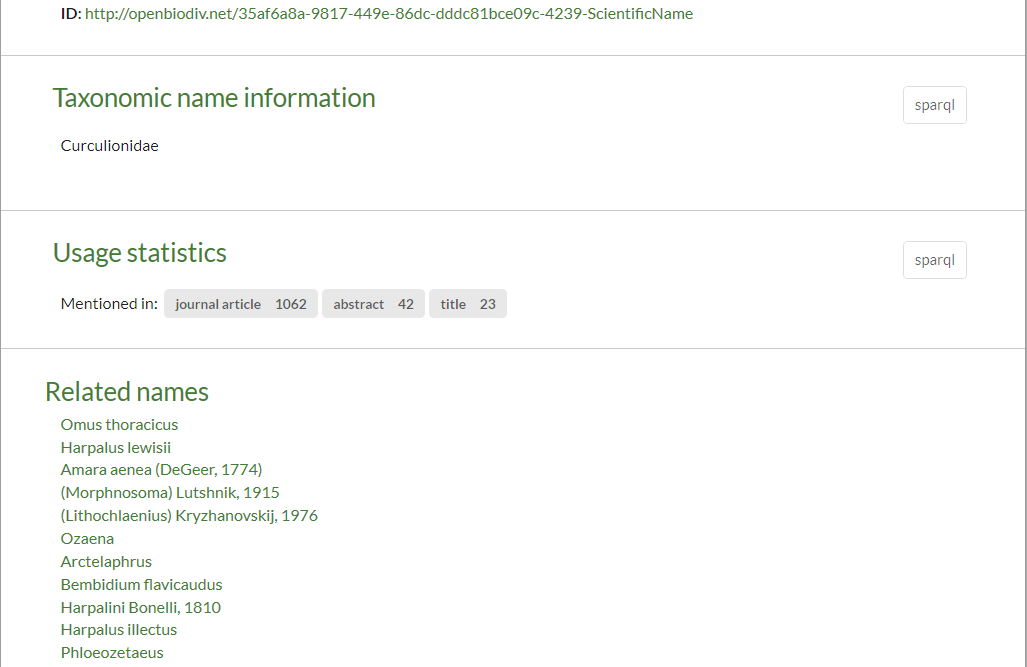
\includegraphics[width=\textwidth]{Figures/portal-name-visualization}
\decoRule
\caption{Visualization.}
\label{fig:portal-name-visualization}
\end{figure}

\subsection{Linking to other resources}

First, all resources in OpenBiodiv form a graph (there are no disconnected parts). The data model is discussed in the next section. Second taxonomic names are linked to external databases via \url{dwc:taxonID}. These are strings containing GBIF ID's, ZooBank ID's, LSID's, etc. Unfortunately as HTTP URI's have not gained popularity in the biodiversity informatics community, the only true resource-id-to-resource-id links are within OpenBiodiv itself. However, we hope that the introduction of OpenBiodiv LOD contributes to the amelioration of this situation.

\section{Data Model}

When creating the RDF graph we have conformed to the OpenBiodiv Ontology described in Chapter~\ref{chapter-ontology} and well-established community ontologies (Fig.~\ref{fig:community-ontologies}). In particular, (1) we use the Semantic Publishing and Referencing Ontologies (SPAR, \cite{peroni_semantic_2014}) to model entities from publishing such as Journal, Article, Section, Figure, Table, and so on; and (2) we use the DarwinCore (DwC, \cite{wieczorek_darwin_2012}) community standard and its extension, the Darwin-SW (\cite{baskauf_darwin-sw:_2016}) ontology, to model entities the biodiversity domain.

\begin{figure}
\centering
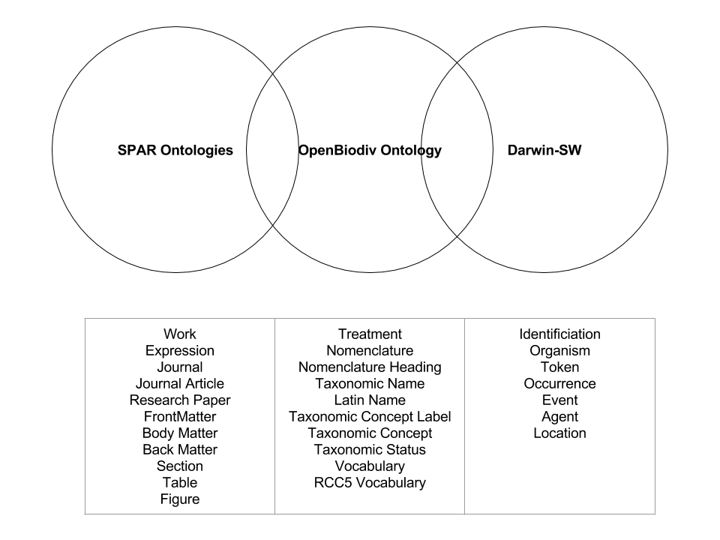
\includegraphics[width=\textwidth]{Figures/community-ontologies}
\decoRule
\caption[Overlap of OpenBiodiv-O with Community Ontologies]{OpenBiodiv-O is an ontology that links the publishing domain with the biodiversity domain. Major resource types covered by each of the ontology families are given in the box below the Venn diagram. Important resources from the publishing domain are listed in the leftmost column and from biodiversity informatics in the rightmost column. The middle one covers important OpenBiodiv-O resources.}
\label{fig:community-ontologies}
\end{figure}

SPAR provides facilities to deal with the dichotomy between the abstract representation of knowledge through the class Work and its concrete representation through the class Expression. For example, a {\tt fabio:JournalArticle} can be the realization of a {\tt fabio:ResearchPaper}. On the other hand, the DwC community standard gives a standard way to express properties from taxonomy and biodiversity science and its extension Darwin-SW a way to reify elements of an occurrence instance such as Identification, Organism, Token, and so on. A caveat: the current version of OpenBiodiv-LOD does not store yet occurrence information but all necessary infrastructure is in place to include them in the next release.

\section{Examples SPARQL queries}

As SPAR, DwC, and OpenBiodiv-O have already been explained elsewhere, we shall illustrate the data model by issuing sample SPARQL queries illuminating aspects of it.

\subsubsection{Query for author} Authors are instances of {\tt foaf:Person} (except in the rare institutional case, in which case they would be {\tt foaf:Agent}'s) and are \emph{creator}-s of Works that have an Expression. The SPARQL query in Listing~\ref{listing:prolific_author} answers the question of which author has been on the author list of the most articles. Note that the results may change as new articles are added to the graph.

\lstinputlisting[language=SPARQL,
caption=Most prolific author SPARQL query.,
label=listing:prolific_author, basicstyle=\ttfamily\tiny]
{Listings/prolific-author.SPARQL.txt}

\subsubsection{Query for scientific name}

Latin names are stored in the system as {\tt :ScientificName}'s are are \emph{mention}-ed by taxonomic name usages.

Listing~\ref{listing:mentioned_name} orders scientific names of any rank by the number of unique mentions that they have in articles. It is possible to narrow down the solution to binomial names (species names) by adding the {\tt dwciri:taxonRank} property as shown in Listing~\ref{listing:mentioned_species_name}. In order to see the different ranks that scientific names are assigned to in OpenBiodiv you can use the query in Listing~\ref{listing:ranks}. It is also possible, for example, to determine the most mentioned scientific name by the number of articles it is mentioned in (Listing~\ref{listing:mentioned_name_articles}).

\lstinputlisting[language=SPARQL,
caption=Most mentioned scientific name.,
label=listing:mentioned_name, basicstyle=\ttfamily\tiny]{Listings/name-mentions.SPARQL.txt}

\lstinputlisting[language=SPARQL,
caption=Most mentioned species name.,
label=listing:mentioned_species_name, basicstyle=\ttfamily\tiny]{Listings/species-name-mentions.SPARQL.txt}

\lstinputlisting[language=SPARQL,
caption=What are the available taxonomic ranks?,
label=listing:ranks, basicstyle=\ttfamily\tiny]{Listings/ranks.SPARQL.txt}

\lstinputlisting[language=SPARQL,
caption=Most mentioned species name by number of articles that mention it.,
label=listing:mentioned_name_articles, basicstyle=\ttfamily\tiny]
{Listings/species-name-mentions-by-articles.SPARQL.txt}

\subsubsection{Query the article structure} A unique feature of OpenBiodiv LOD is that articles are broken down into their components (see e.g. Table~\ref{datatypes-taxpub-taxonx} later in this Chapter) and mentions (e.g. taxonomic name usages) connect to the specific part of the article and not just to the article in general.

Combining this feature with queries from the previous paragraph, we can, for example, look for the most mentioned scientific name in a figure (Listing~\ref{listing:mentioned_name_figures}). The only difference in this query is that we have replaced the type of {\tt ?a} with {\tt doco:Figure}. 

\lstinputlisting[language=SPARQL,
caption=Most mentioned scientific name in figures,
label=listing:mentioned_name_figures, basicstyle=\ttfamily\tiny]
{Listings/name-mentions-by-figure.SPARQL.txt}

We can look, for example, for the figures present in a particular article (Listing~\ref{listing:figures_article})

\lstinputlisting[language=SPARQL,
caption=Figures of a given article., label=listing:figures_article, basicstyle=\ttfamily\tiny]
{Listings/figures-of-article.SPARQL.txt}

\subsubsection{Query for taxonomic concepts}

A key feature of OpenBiodiv-O is that it allows for the separation of taxonomic concepts from scientific names. Scientific names are linked both to the components of an article that mentions them and to taxonomic concepts. To illustrate this, we can create a query uniting information from concepts from the GBIF Backbone Taxonomy (next subsection) with semantics coming from the article structure. The query in Listing~\ref{listing:new_curcu} locates the beetle family Curculionidae sec. \cite{gbif_secretariat_gbif_2017} in the system, and looks for new taxa ({\tt :TaxonomicDiscovery}) that have been associated with one of its genera.

\lstinputlisting[language=SPARQL,
caption=Taxonomic discoveries in the weevils., label=listing:new_curcu, basicstyle=\ttfamily\tiny]
{Listings/new-curculionidae.SPARQL.txt}

\subsubsection{Fuzzy Queries via Lucene}

The SPARQL endpoint of OpenBiodiv LOD supports fuzzy matching via a Lucene connector (\cite{ontotext_graphdb_2018}). In taxonomy, this can be a very useful as due to multiplicity of taxonomic names and the complexities of Latin grammar, one often does not remember the correct spelling of a name. This can lead to no matches in an exact search even though the system may contain information about that name.

Lucene queries at the OpenBiodiv workbench are made in SPARQL. In order to carry out a Lucene query, one matches the following graph patter. A search variable is defined of type \url{http://www.ontotext.com/connectors/lucene/instance#WordSearch}. Then the Lucene query that needs to follow the standard Lucene query syntax (\cite{the_apache_software_foundation_apache_2013}) is specified as a literal string of the property \url{http://www.ontotext.com/connectors/lucene#query} of the search variable:

\lstinputlisting[style=customsparql,
caption=Sample Lucene query via SPARQL. We have intentionally misspelled the person's name., label=listing:replacement-name]
{ Listings/sample-lucene-query.SPARQL.txt}

In the above query \cl{?search} defines an object of type \cl{inst:WordSearch} for the query. The search results are specified by linking the search object to \cl{?resource} via \cl{lucene:entities}. Finally \cl{?resource} has a \cl{lucene:score} property indicating how close was the guess. It is hard to quantify the meaning of the scores in absolute terms but it is always the case that a higher score is closer to the true text than a lower one.

\subsubsection{Competency question answering via SPARQL}

At the end of Chapter~\ref{chapter-ontology} we suggested some competency questions that may be answered by OpenBiodiv. Of central importance is the question of whether a given taxonomic name is valid or not. We shall consider a taxonomic name invalid from the viewpoint of the information made available to OpenBiodiv if and only if at least one of the following invalidation criteria holds:

\begin{enumerate}
\item{The name has been replaced. I.e. there is a {\tt :replacementName} property originating in the name and there are no loops: it is impossible to follow the {\tt :replacementName} edges and come back to the name. This query is illustrated in Listing~\ref{listing:replacement-name}}.
\item{The name has been invalidated, i.e. there is a taxonomic usage with the status {\tt :UnavailableName} and there is no newer taxonomic name usage revalidating it ({\tt :AvailableName}). Illustrated in Listing~\ref{listing:unavailable-name}.}
\end{enumerate}


\lstinputlisting[language=SPARQL,
caption=Asks if the name given by the label has been replaced., label=listing:replacement-name, basicstyle=\ttfamily\tiny]
{Listings/ask-replacement-name.SPARQL.txt}

\lstinputlisting[language=SPARQL,
caption=Asks if the name given by the label is considered unavailable., label=listing:unavailable-name, basicstyle=\ttfamily\tiny]{Listings/ask-unavailable.name.SPARQL.txt}


\section{Dataset Generation}

In the previous section on sources we examined the data formats that each source provides. The inputs are either XML (Pensoft and Plazi) or CSV (GBIF). Thus, the raw data-streams are semi-structured and the dataset generation problem can be thought of as an information retrieval and transformation problem. The input is encoded in three different data models---DarwinCore CSV (GBIF), TaxPub XML (Pensoft), and TaxonX XML (Plazi). The output of the transformation pipeline is  knowledge represented in a fully-structured way according to the ontology.

\subsection{Obtaining the data}

The first step before running any transformation is to obtain the raw inputs. GBIF's taxonomic backbone is available under\\ 
\url{<https://www.gbif.org/dataset/d7dddbf4-2cf0-4f39-9b2a-bb099caae36c>}.\\There is an RSS feed from which Plazi's treatments can be downloaded on a daily basis under \url{<http://tb.plazi.org/GgServer/xml.rss.xml>}. Each of Pensoft's journals has a public API endpoint under \url{<http://[journal_name].pensoft.net/lib/journal_archive.php>}, where \url{[journal_name]} ought to be replaced with the name of the Pensoft journal. E.g. {\tt bdj} to make \url{<http://bdj.pensoft.net/lib/journal_archive.php>}.



\subsection{Tools}

In order to carry out the dataset generation we made use of the following tools:

\begin{enumerate}
\item{RDF4R R package\footnote{RDF4R package on GitHub \href{https://github.com/vsenderov/rdf4r}{\url{<https://github.com/vsenderov/rdf4r>}}}, which is described in Chapter~\ref{chapter-rdf4r} and deals with all RDF-related issues such as accessing a triple store, serializing the in-memory resource representations to Turtle files, etc.}
\item{ROpenBio R package\footnote{ROpenBio R package on GitHub \href{https://github.com/pensoft/ropenbio}{\url{<https://github.com/pensoft/ropenbio>}}}, which implements the data retrieval and transformations described in this chapter.}
\item{TSV4RDF, which is a PHP library for mapping CSV to RDF developed by Pensoft. It is closed-source and developed outside of the scope of the dissertation and is not discussed in detail.}
\item{The OpenBiodiv base\footnote{OpenBiodiv Base \href{https://github.com/vsenderov/OpenBiodiv}{\url{<https://github.com/vsenderov/OpenBiodiv>}}}, which contains scripts needed for the initialization and updating of the database.}
\end{enumerate}

In the rest of the section we describe the transformation from XML as it is implemented in ROpenBio. We do not describe the TSV4RDF transformation of GBIF to RDF as it is a closed source product.

\subsection{XML to RDF transformation}

In order to transform an article represented as an XML document to RDF, we make use of the hierarchical nature of XML and solve the problem recursively with the following Extractor procedure in Algorithm~\ref{algo:extractor}. The extractor's procedure input is an XML node and its output is the RDF corresponding to the XML node. The extractor procedure has three essential steps: atoms extraction, RDF constructions from the extracted atoms, a divide-and-conquer step that recursively calls itself and unites the results. Extraction of a whole article is achieved by calling the Extractor on the root node of the article.

% http://tug.ctan.org/macros/latex/contrib/algorithmicx/algorithmicx.pdf
\begin{algorithm}
\caption{The Extractor procedure}
\begin{algorithmic}[1]
\Procedure {Extractor}{XML Node $X$}
\State $a \leftarrow$ extract atoms of $X$
\Comment Atoms extraction
\State $r \leftarrow$ construct RDF from $a$
\Comment RDF construction
\State $C \leftarrow$ find relevant sub-nodes of $X$
\Comment Recursively applies itself
\State $R \leftarrow$ apply Extractor on each $C_i \in C$
\State \Return $r \bigcup R$
\EndProcedure
\end{algorithmic}
\label{algo:extractor}
\end{algorithm}

\subsubsection{Atoms extraction}

The atoms of an XML node consist of all text-fields that can be reached from the XML node with an XPATH expression (can be attribute values or text values) that can be directly converted to RDF as literals or identifiers. They all belong to one or to several related RDF resources. For example in Listing~\ref{listing:author-xml-snippet} we have listed the XML node that contains author information in the TaxPub schema. The atoms here are {\tt surname = "Wachkoo"}, {\tt given\_name = "Aijaz Ahmad"}, {\tt orcid\_id = "https://orcid.org/0000-0003-2506-9840"}, {\tt affiliation = "Central Institute of Temperate Horticulture, Srinagar, Jammu \& Kashmir, India"}. In order to achieve the extraction, the atoms extractor must know the XPATH locations (e.g. the surname is at {\tt ./name/surname}) of the authors it is looking for and the types of the values (e.g. string, integer, link, etc.). Sometimes this can be quite challenging as is the affiliation field in the given example. In it the XPATH location of the address string is influenced by the value of {\tt xref}. In other words we have here that the address line is stored at "{//aff[id=./xref/@rid]}"; however, this syntax may be invalid some XPATH libraries and additional processing outside of XPATH may be required!

\begin{lstlisting}[language=XML,
caption=XML snippet of an author.,
label=listing:author-xml-snippet, basicstyle=\ttfamily\tiny]
<contrib contrib-type="author" corresp="no">
  <name name-style="western">
    <surname>Wachkoo</surname>
    <given-names>Aijaz Ahmad</given-names>
  </name>
  <uri content-type="orcid">https://orcid.org/0000-0003-2506-9840</uri>
  <xref ref-type="aff" rid="A3">3</xref>
</contrib>  

<aff id="A3">
 <label>3</label>
 <addr-line>
   Central Institute of Temperate Horticulture, Srinagar, Jammu & Kashmir, India
 </addr-line>
</aff>
\end{lstlisting}

\subsubsection{RDF Generation}

Once the atoms have been extracted they can be put together as RDF. Conceptually this is straightforward as for each atom we know the type of each atom and therefore we know which RDF property to use. The author example is given in Listing~\ref{listing:author_rdf}.

It should be noted in this paragraph that the semantics of certain node types such as taxonomic name usage (reified as {\tt :TaxonomicNameUsage}) reflect the relative position of the node in the XML document. For example, a taxonomic name usage may be inside a figure, inside an introduction section, inside a title, etc. Therefore besides the atoms, the constructor receives information about the relative position of the resource in the article by means of the unique identifier of the parent node(s). Then this information is encoded in RDF as given in Listing~\ref{listing:parent-node-rdf}. 

\begin{lstlisting}[language=SPARQL,
caption=RDF snippet of an author. This is a somewhat idealized situation in which the language of the address was available from the article., label=listing:author_rdf, basicstyle=\ttfamily\tiny]
@prefix rdf: <http://www.w3.org/1999/02/22-rdf-syntax-ns#> .
@prefix foaf: <http://xmlns.com/foaf/0.1/> .

:a a foaf:Person ;
   rdfs:label "Aijaz Ahmad Wachkoo".
   :affiliation "Central Institute of Temperate Horticulture, Srinagar, Jammu & Kashmir, India"@en ;
   foaf:familyName "Wachkoo" ;
   foaf:givenName "Aijaz Ahmad" .
\end{lstlisting}

\begin{lstlisting}[language=SPARQL,
caption=., label=listing:parent-node-rdf, basicstyle=\ttfamily\tiny]
:2b836ad5-db56-4093-9752-33c9f7892de6   rdf:type   fabio:JournalArticle ;
  rdfs:label   "Changes to publication requirements made at the XVIII Internation\
al Botanical Congress in Melbourne - what does e-publication mean for you?" ;
  dc:title   "Changes to publication requirements made at the XVIII International\
 Botanical Congress in Melbourne - what does e-publication mean for you?" ;
 prism:doi   "10.3897/mycokeys.1.1961" ;
 dc:publisher   "Pensoft Publishers" ;
 prism:publicationDate   "2011-9-14"^^xsd:date ;
 dcterms:publisher   openbiodiv:0df76aab-1fcf-4118-8e50-198e830a7bed .
 openbiodiv:151a37ba-a337-4855-8e01-200f5ec0251b   rdf:type   deo:Introduction ;
         po:isContainedBy   openbiodiv:2b836ad5-db56-4093-9752-33c9f7892de6 .
}
\end{lstlisting}

\subsubsection{Divide and conquer}

After we have successfully converted the current XML node to RDF, a recursive call to Extractor is made for all nodes that are hierarchically dependent on the current node. For example, the article node contains all the other other nodes such as sections, figures, etc.

\subsubsection{Transformation specification}

In order for the Extractor to work, therefore, we need to specify an XML schema. The specification includes what XML nodes we are looking for and their location. It then recursively specifies for each node, what sub-nodes we are looking for and their XPATH location relative to their parent node. Finally, for every node we need to give the atom locations and write a constructor. The transformation specification is done with R6 framework in R. We have specified two schemata that share the same constructors---TaxPub\footnote{\url{https://github.com/pensoft/ropenbio/blob/redesign/R/taxpub.R}} and TaxonX\footnote{\url{https://github.com/pensoft/ropenbio/blob/redesign/R/taxonx.R}}.

\subsection{Submission to graph database and post-processing}

In the previous section we described how we transform XML documents in TaxPub and TaxonX to RDF statements according to OpenBiodiv-O. In addition, we transform the GBIF backbone taxonomy to RDF according to OpenBiodiv-O with the help of TSV4RDF, a proprietary Pensoft tool. The generated RDF statements are submitted to a repository in a GraphDB instance residing on \url{http://graph.openbiodiv.net/}. The repository has been initialized with OpenBiodiv-O and the ontologies on which it depends\footnote{\url{https://github.com/vsenderov/openbiodiv-o/tree/master/imports}}. Finally, after the data has been submitted, update scripts are run to generate further statements from our ontology that have not been encoded in OWL for the updating of scientific name relations.

\subsubsection{Update rule for replacement name}

We state that a scientific name $A$ replaces a scientific name $B$, if there exists a taxonomic name usage of $A$ with taxonomic status {\tt :ReplacementName} and $B$ is mentioned by a taxonomic name usage in the nomenclatural citations of the treatment, where the discussed taxonomic name usage of $A$ is in the nomenclature section (Listing~\ref{listing:update_replacement_name}).

\lstinputlisting[language=SPARQL,
caption=Update rule for replacement name.,
label=listing:update_replacement_name, basicstyle=\ttfamily\tiny]{Listings/update-replacement-name.SPARQL.txt}

\subsubsection{Update rule for related name}

The related names update-rule is similar to the replacement name: two scientific names $A$ and $B$ are consider related if they both mentioned in the nomenclature section of a treatment (Listing~\ref{listing:update_related_name}).

\lstinputlisting[language=SPARQL,
caption=Update rule for related name.,
label=listing:update_related_name, basicstyle=\ttfamily\tiny]{Listings/update-related-name.SPARQL.txt}

\section{Performance degradation analysis}

The current iteration of the database holds over 600 million triples (Fig.~\ref{fig:statements-report}). The expansion ratio under the RDFS-Plus (Optimized) ruleset is 2.35, i.e. for each asserted statements we materialize on average 2.35 implicit statements. Under the OWL2-RL ruleset (which contains a full implementation of OWL logic rules), the expansion ratio is about 3.7; however, we encountered significant performance issues using it (Fig.~\ref{fig:performance-degradation}). Even with the lighter ruleset (RDFS-Plus Optimized), we still see performance degradation with increasing database size. Importing the GBIF backbone taxonomy from file takes about two days under the easier scenario. The subsequent importing of the Pensoft archives takes about two weeks as it is a slower operation requiring not only the time for submission but the time for converting the XML's to RDF.

\begin{figure}
\centering
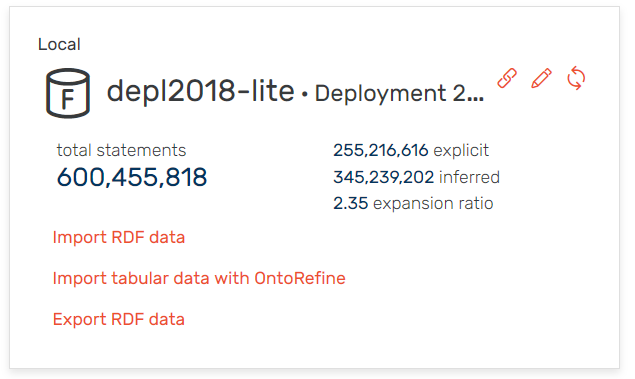
\includegraphics[width=\textwidth]{Figures/active-repository}
\decoRule
\caption[Statements report]{Statements report from the GraphDB workbench.}
\label{fig:statements-report}
\end{figure}

\begin{figure}
\centering
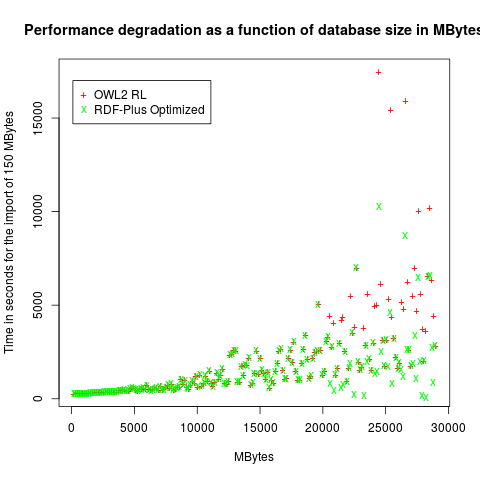
\includegraphics[width=\textwidth]{Figures/performance-degradation-both}
\decoRule
\caption[Performance degradation]{The graph visualizes the time in seconds needed to import a 150 MB big Turtle data file as a function of the database size. The database size is measured by the adding up the size of the data files that have already been imported.}
\label{fig:performance-degradation}
\end{figure}


\chapter{RDF4R: R Library for Working with RDF}
\label{chapter-rdf4r}

RDF4R ({\tt rdf4r}) is an R package for working with Resource Description Framework (\cite{rdf_working_group_resource_2014}) data. It was developed as part of the OpenBiodiv project but is completely free of any OpenBiodiv-specific code and can be used for generic purposes requiring tools to work with RDF data in the R programming environment (\cite{r_core_team_r:_2016}).

\section{Installation}

RDF4R depends on the following packages (list may change in future releases):

\begin{itemize}
\item{{\tt gsubfn} (\cite{grothendieck_gsubfn:_2018})}
\item{{\tt httr} (\cite{wickham_httr:_2017})}
\item{{\tt xml2} (\cite{wickham_xml2:_2018})}
\item{{\tt R6} (\cite{chang_r6:_2017})}
\item{{{\tt devtools} (\cite{wickham_devtools:_2018})}---needed if one is to do a GitHub install.}
\end{itemize}

Installation of the above packages via {\tt install.packages} is needed to use RDF4R. Pay attention to error messages during their installation as additional OS-level components may need to be installed.

Install RDF4R from GitHub with the following command:

\begin{lstlisting}[language=R,
basicstyle=\ttfamily\tiny]
devtools::install_github("vsenderov/rdf4r")
\end{lstlisting}

We are currently in the process of submitting the package to a repository and making it available through the standard installation facilities of R. Our intention is to publish it through CRAN and/or rOpenSci\footnote{Repositories accessible under \url{https://cran.r-project.org/} and \url{https://github.com/ropensci/}, respectively}.

\section{Specification}

RDF4R has the features listed in the following subsections.

\subsection{Connection to a triple-store}

Triple-stores, also known as quad-stores, graph databases, or semantic databases, are databases that store RDF data and allow the querying of RDF data via the SPARQL query language (\cite{the_w3c_sparql_working_group_sparql_2013}). RDF4R can connect to triple-stores that support the RDF4J server REST API (\cite{rdf4j_development_team_rdf4j_2017}) such as GraphDB (\cite{ontotext_graphdb_2018}). It is possible to establish both basic connections (requiring no password or requiring basic HTTP user-pass authentication) or connection secured with an API access token.

\subsection{Work with repositories on a triple-store}

Once a connection to a triple-store has been established, it is possible to inspect the talk protocol version, view the list of repositories on the database, execute SPARQL Read (SELECT keyword and related) and SPARQL Update (INSERT and related) queries on the database, as well as submit serialized RDF data directly to the database.

\subsection{Function factories to convert SPARQL queries to R functions}

An important feature of RDF4R are its facilities for converting SPARQL queries and the like to R functions. This conversion is realized by a family of functions that return functions. In this thesis they will be referred to as function factories. Taking the example of the {\tt query\_factory} we have: given a parameterized SPARQL query (parametrization syntax is explained later), {\tt query\_factory} returns a function $f$ whose arguments are the parameters of the query. Upon being called $f$ submits the query to a SPARQL endpoint and returns the results.

\subsection{Work with literals and identifiers}

The building blocks of RDF are literals (e.g. strings, numbers, dates, etc.) and resource identifiers. RDF4R provides classes for literals and resource identifiers that are tightly integrated with the other facilities of the package.

\subsection{Prefix management}

Prefixes are managed automatically during serialization by being extracted from the resource identifiers.

\subsection{Creation and serialization of RDF}

RDF4R uses an own implementation of smart dynamically reallocated vector data structure to store RDF triples as mutable R6 objects. Blank nodes are partially supported: a triple may contain an anonymous RDF object (a list of triples with the same subject) as its third position. In this case, the parent RDF is serialized as Turtle by using the bracket syntax (Listing~\ref{fig:turtle-brackets}). Currently, the serialization procedure only supports Turtle (and its variant Trig, \cite{bizer_rdf_2014}) and only supports adding new triples.

\begin{lstlisting}[language=SPARQL,
caption=Using brackets to express RDF blank nodes in Turtle/TriG.,
label=fig:turtle-brackets,
basicstyle=\ttfamily\tiny]
@prefix foaf: <http://xmlns.com/foaf/0.1/> .

# :someone knows someone else, who has the name "Bob".
:someone foaf:knows [ foaf:name "Bob" ] .
\end{lstlisting}

\subsection{A basic vocabulary of semantic elements}

RDF4R has some basic resource identifiers for widely used classes and predicates predefined (e.g. for {\tt rdf:type}, {\tt rdfs:label}, etc.).

\section{Usage}

Here, we explain how to use the package RDF4R by means of examples. In order to fully utilize the package capabilities, one needs to have access to an RDF graph database. We have made available a public endpoint (see next paragraph) to allow the users of the package to experiment. Since write access is enabled, please be considerate and don't issue catastrophic commands.

\subsection{Connection to triple store}

The code in Listing~\ref{fig:rdf4r-connecting-graphdb} creates an object, {\tt graphdb}, that stores the information needed to access the database. The user needs to supply it to the access functions discussed later. We have also created an object {\tt openbiodiv} that contains read-only access to the main OpenBiodiv instance. All examples in this section use one of these two access points.

\begin{lstlisting}[language=SPARQL,
caption=R code: connecting to an RDF database using RDF4R. Outputs are given as comments after the statements.,
label=fig:rdf4r-connecting-graphdb,
basicstyle=\ttfamily\tiny]
library(rdf4r)

openbiodiv = rdf4r::basic_triplestore_access(
  server_url = "http://graph.openbiodiv.net",
  repository = "depl2018-lite"
)

graphdb = rdf4r::basic_triplestore_access(
  server_url = "http://graph.openbiodiv.net",
  user = "dbuser",
  password = "public-access",
  repository = "test"
)

graphdb
# $server_url
# [1] "http://graph.openbiodiv.net"
# $repository
# [1] "test"
# $authentication
# <request>
# Options:
# * httpauth: 1
# * userpwd: dbuser:public-access
# $status
# [1] 8
# attr(,"class")
# [1] "list"                       "triplestore_access_options"

openbiodiv
# $server_url
# [1] "http://graph.openbiodiv.net"
# $repository
# [1] "depl2018-lite"
# $authentication
# NULL
# $status
# [1] 8
# attr(,"class")
# [1] "list"                       "triplestore_access_options"

get_protocol_version(graphdb)
# [1] 8

list_repositories(graphdb)
# uri             id readable writable
# 1         http://graph.openbiodiv.net/repositories/SYSTEM         SYSTEM     true     true
# 2 http://graph.openbiodiv.net/repositories/depl2018-mini2 depl2018-mini2     true     true
# 3       http://graph.openbiodiv.net/repositories/depl2018       depl2018     true     true
# 4           http://graph.openbiodiv.net/repositories/test           test     true     true
# 5  http://graph.openbiodiv.net/repositories/depl2018-lite  depl2018-lite     true     true
\end{lstlisting}

\subsection{Example: convert a SPARQL query to an R function}

The purpose of this example is to convert a simple SPARQL lookup query to an R function. The publicly accessible endpoint happens to store some biological information but for the purposes of this example knowledge of biological taxonomy or the ontology of the store is irrelevant. It is only necessary to know that the database stores information about biological papers that contain references to biological names. We are looking for papers that mention the biological name \emph{Drosophila}, which is a genus of flies. Please note the parametrization of the SPARQL query.

\lstinputlisting[language=R,
caption=R. Parameterized SPARQL query to lookup a genus in OpenBiodiv.,
label=listing:update_replacement_name, basicstyle=\ttfamily\tiny]{Listings/update-replacement-name.SPARQL.txt}

Note that this almost valid SPARQL with one exception - the {\tt \%param} string on the first line of the WHERE clause. A SPARQL query is parameterized by specifying a \% in front of the tokens that have to become the arguments of the generated R function. Construction of a function follows that looks up a genus (a biological rank) by a supplied string.

\begin{lstlisting}[language=R,
basicstyle=\ttfamily\tiny]
genus_lookup = rdf4r::query_factory(p_query = p_query, access_options = openbiodiv)
\end{lstlisting}

{\tt query\_factory} takes two arguments: the parameterized query and an object with access options for an endpoint and returns an R function whose arguments are the parameters of the parameterized SPARQL query and which executes the SPARQL query against the endpoint specified in {\tt access\_options} and returns formatted results as a dataframe.

\begin{lstlisting}[language=R,
basicstyle=\ttfamily\tiny]
genus_lookup("\"Drosophila\"")
#    genus title
# 1   Drosophila  Characterisation of the chemical profiles of Brazilian and Andean
# morphotypes belonging to the Anastrephafraterculus complex (Diptera, Tephritidae)
# 2   Drosophila                A new species group in the genus Dichaetophora, with
# descriptions of six new species from the Oriental region (Diptera, Drosophilidae)
\end{lstlisting}

Note that we have enclosed the string {\tt Drosophila} in escaped quotes as only that would make the replacement of the parameter in the parameterized SPARQL query a valid SPARQL. Had the parameter been a resource identifier, we would not have needed the quotes. In a later example, we will show how we can get around this hassle by utilizing the built-in classes for literals and resource identifiers.

\paragraph{Excercise.} Try experimenting with {\tt genus\_lookup} by looking up information about some other genera (\emph{Eupolybothrus} - a millepede, \emph{Myotis} - a bat).

\subsection{Setting up literals and identifiers}

We want to model Table~\ref{table:classical-works} (recreated from Alemang and Hendler 2008). We will use the prefix \url{<http://rdflib-rdf4r.net/>} for all instances that we create and a dummy ontology (not actually defined) with the prefix \url{<http://art-ontology.net/>} to reify the example classes and properties.

\begin{table}[h!]
\caption{Tabular Data about Elizabethan Literature and Music recreated from \cite{allemang_semantic_2011}.}
\begin{tabular}{ccccc}
\hline
 ID & Title                       & Author            & Medium & Year\\  \hline
 1  & \emph{As You Like It}       & Shakespeare       & Play & 1599\\
 2  & \emph{Hamlet}               & Shakespeare       & Play & 1604\\
 3  & \emph{Othello}              & Shakespeare       & Play & 1603\\
 4  & "Sonnet 78"                 & Shakespeare       & Poem & 1609\\
 5  & \emph{Astrophil and Stella} & Sir Philip Sidney & Poem & 1590\\
 6  & \emph{Edward II}            & Christopher Marlowe  & Play & 1590\\
 7  & \emph{Hero and Leander}     & Christopher Marlowe  & Poem & 1593\\
 8  & Greensleeves                & Henry VIII Rex       & Song & 1525
\end{tabular}
\label{table:classical-works}
\end{table}

\subsubsection{Literals}

In Listing~\ref{listing:literal-construction}, we repeatedly called the {\tt literal} function, which is a constructor of objects of class \emph{literal}, with different arguments. {\tt literal} can construct phrases in English (or any other language) with the {\tt lang} argument. It can construct pure strings (by omitting the {\tt lang} argument) of type {\tt xsd:string}. It can also construct literals of a number of defined semantic types by using the {\tt xsd\_type} argument. In order to see which types are available execute {\tt ?semantic\_elements}. Note that the XSD types are implemented as resource identifiers (class \emph{identifier}), which allows the user to implement additional types that are not provided. Behind the scenes the URL of the resource identifier will be appended to the representation ({\tt ?represent}) of the literal as text through pasting of {\tt \textasciicircum\textasciicircum} and then the URL.

\lstinputlisting[language=R,
caption=R. Literal construction.,
label=listing:literal-construction, basicstyle=\ttfamily\tiny]{Listings/literal-construction.R.txt}

In other words, for the work titles, we use the argument {\tt lang="en"} telling the literal constructor that the literal value is in English, whereas for the names, we omit this argument. As per semantic web conventions, when the argument is omitted, and no type is explicitly specified, it is assumed that the literal is a string ({\tt xsd:string}). For the literals containing years, on the other hand, we explicitly specify an integer type; otherwise they would have parsed as strings as well. All of this can be seen by inspecting the individual lists (objects of class \emph{literal} are lists):

\lstinputlisting[language=R,
caption=R. Representation of literals.,
label=listing:literal-representation, basicstyle=\ttfamily\tiny]{Listings/representation-literals.R.txt}

\subsubsection{Identifiers}

We need resource identifiers for our resources, i.e. playwrights, works of art, as well as for the classes of which those resources are instances of. To make things simpler, we use a fictional ontology with the prefix \url{<http://art-ontology.net/>}. We hardcode identifiers for the ontology classes:

\lstinputlisting[language=R,
caption=R. Entering identifiers.,
label=listing:some-identifiers, basicstyle=\ttfamily\tiny]{Listings/some-identifiers.R.txt}

Inspection of one class and one property:

\lstinputlisting[language=R,
caption=R. Entering identifiers.,
label=listing:some-identifiers, basicstyle=\ttfamily\tiny]{Listings/identifier-representation.R.txt}

Note that each identifier object is a list where the field {\tt \$uri} gives the URI of the resource and the field {\tt qname} gives the shortened name (QNAME) with respect to the prefix stored in {\tt \$prefix}. Also note that both literal and identifier are representable, i.e. we have defined a the generic represent on both of the classes that outputs a proper string representation of the literal or resource identifier that can be used in a serialization.

We also need resource identifiers for our entities such as Shakespeare, Christopher Marlowe, etc. Semantic Web best practices discourage the liberal minting of identifiers for resources for which somebody has already minted an identifier. Instead, we want to look them up in a database, and only mint if they are not found. For this, RDF4R offers factory functions to create lookup/mint functions as seen in Listing~\ref{listing:id-factory}.

\lstinputlisting[language=R,
caption=R. Identifier factory.,
label=listing:id-factory, basicstyle=\ttfamily\tiny]{Listings/id-factory.R.txt}

{\tt identifer\_factory}'s first argument, {\tt fun}, is a list of (lookup) functions that will be tried. {\tt identifier\_factory} returns an identifier constructor function, in our case we named it {\tt lookup\_or\_mind\_id}. The lookup functions need to return a single column (labeled e.g. {\tt ?id}). They will be tried in order and if any of them returns a unique solution, it will be returned by the constructor function to create an identifier object. If none of the lookup functions returns a unique solution, a new identifier will be minted. 

\subsection{Creating RDF}

To create an RDF representation, create a new {\tt ResourceDescriptionFramework} object and add triples to it (Listing~\ref{listing:rdf-representation}).

\lstinputlisting[language=R,
caption=R. Creating RDF.,
label=listing:rdf-representation, basicstyle=\ttfamily\tiny]{Listings/rdf-representation.R.txt}

The easiest way to inspect the {\tt ResourceDescriptionFramework} object is to serialize it. Before we serialize, however, we need to specify the subgraph where the triples should be stored with {\tt \$set\_context(id)}. We will reuse the example for that.

\begin{lstlisting}[language=R,
basicstyle=\ttfamily\tiny]
classics_rdf$set_context(identifier(id = "classic_example", prefix  = eg))
cat(classics_rdf$serialize())
# @prefix example: <http://rdflib-rdf4r.net/> .
# @prefix art: <http://art-ontology.net/> .
# @prefix rdfs: <http://www.w3.org/2000/01/rdf-schema#> .
# @prefix rdf: <http://www.w3.org/1999/02/22-rdf-syntax-ns#> .
# example:classic_example {
# example:0bac3b32-8aac-11e8-a1c9-c961fe5afe72   art:wrote   example:0aeae996-8aac-11e8-a1c9-c961fe5afe72 ,  example:0aff274e-8aac-11e8-a1c9-c961fe5afe72 . 
# example:0aeae996-8aac-11e8-a1c9-c961fe5afe72   rdfs:label   "King Lear"@en . 
# example:0aff274e-8aac-11e8-a1c9-c961fe5afe72   rdfs:label   "As You Like It"@en ;
#	 art:has_year   "1599"^^xsd:integer ;
#	 rdf:type   art:Play .
# }
\end{lstlisting}

\subsection{Submitting RDF to the triple store}

Now that we have created some RDF ({\tt classics\_rdf}), we are ready to submit it to the endpoint ({\tt graphdb}). We can either submit it directly via {\tt add\_data}, or we can use the {\tt add\_data\_factory} to create a submitter function.

\begin{lstlisting}[language=R,
basicstyle=\ttfamily\tiny]
# via add_data
add_data(classics_rdf$serialize(), access_options = graphdb)
simple_lookup(represent(lking_lear))
# id
# 1 http://rdflib-rdf4r.net/0aeae996-8aac-11e8-a1c9-c961fe5afe72
simple_lookup(represent(lking_lear))
# id
# 1 http://rdflib-rdf4r.net/0aeae996-8aac-11e8-a1c9-c961fe5afe72
p_query_describe = "PREFIX example: <http://rdflib-rdf4r.net/>
+ SELECT ?p ?o
+ WHERE {
+ %resource ?p ?o .
+ }"
describe = query_factory(p_query = p_query_describe, access_options = graphdb)
describe(represent(idshakespeare))
# p                                                            o
# 1 http://art-ontology.net/wrote http://rdflib-rdf4r.net/0aeae996-8aac-11e8-a1c9-c961fe5afe72
#2 http://art-ontology.net/wrote http://rdflib-rdf4r.net/0aff274e-8aac-11e8-a1c9-c961fe5afe72
describe(represent(idas_you_like_it))
#               p                            o
# 1 http://www.w3.org/1999/02/22-rdf-syntax-ns#type http://art-ontology.net/Play
# 2      http://www.w3.org/2000/01/rdf-schema#label               As You Like It
# 3                http://art-ontology.net/has_year                         1599
\end{lstlisting}

\section{Discussion}

\subsection{Related Packages}

The closest match to RDF4R is the {\tt rdflib} (\cite{boettiger_rdflib:_2018}). The development of the two packages was simultaneous and independent until {\tt rdflib}'s first official release on Dec 10, 2017. This explains why two closely related R packages for working with RDF exist. After the release of {\tt rdflib} work was started  to make both packages compatible with each other. In our opinion, the packages have different design philosophies and are thus complementary.

{\tt rdflib} is a high-level wrapper to {\tt redland} (\cite{jones_redland:_2016}), which is a low-level wrapper to the C {\tt librdf} (\cite{beckett_redland_2014}), a powerful C library that provides support for RDF. {\tt librdf} provides an in-memory storage model for RDF beyond what is available in RDF4R and also persistent storage working with a number of databases. It enables the user to query RDF objects with SPARQL. Thus, {\tt librdf} can be considered a complete graph database implementation in C.

In our opinion, {\tt redland} is more complex than needed for the purposes of OpenBiodiv. By the onset of the OpenBiodiv project it was available\footnote{But not {\tt rdflib}!}; however, we decided not to use it as a decision was made to rely on GraphDB for our storage and querying. Note that RDF4R's main purpose is to provide a convenient R interface for users of GraphDB and similar RDF4J compatible graph databases.

A feature that differentiates {\tt rdflib} from RDF4R is the design philosophy. RDF4R was designed primarily with the Turtle and TriG serializations in mind. This means that RDF4R can work with named graphs, whereas their usage is discouraged or perhaps impossible with {\tt rdflib}\footnote{The issue was discussed on the {\tt librdf} GitHub page, \url{https://github.com/ropensci/rdflib/issues/23}.}, even though {\tt rdflib}'s default format is N-Quads.

Another differentiating feature between RDF4R and {\tt rdflib} is that RDF4R provides facilities for converting SPARQL and related statements to native R functions!

In a future release of RDF4R (2.0) we would like to replace or extend its in-memory model with {\tt rdflib}'s. This is why we would like to make the packages fully compatible and have contributed several patches to {\tt rdflib}\footnote{Please, consult the commit history under \url{https://github.com/ropensci/rdflib}.}). Thus, it will be possible for the user of RDF4R to retain its syntax and high-level features--- constructor factories, functors, etc., and the ability to use named graphs---but benefit from performance increases, stability, and scalability with the {\tt redland/rdflib/librdf} backend.

This will enable the users of the R programming environment to use whichever syntax they prefer and benefit from an efficient storage engine.

\subsection{Elements of Functional Programing (FP)}

When choosing a programming environment for the project, a choice was made to use R (\cite{r_core_team_r:_2016}) given its ubiquity in data science. Having settled on R, we decided to incorporate elements of the functional programming style (\cite{wickham_advanced_2015}) that R supports in order to allow the users of the package to write simple code to solve complex tasks.

RDF4R is not written as in a pure functional programming style: some of its functions have side-effects. However, we make use of functions as first-class citizens and closures. By ``functions as first-class citizens'' we mean that RDF4R has both functions that return functions and functions that take functions as arguments.

The simplest example of such a function is the {\tt query\_factory} function which converts a SPARQL query to an R function. We believe that this is a very useful feature because the working ontologist often has quite a few SPARQL queries that they want to execute and then parse the results of. Had we just provided the generic {\tt submit\_sparql} function, the workflow for the user would have looked as follows: first, modify the SPARQL query somehow (e.g. by for example changing a label that is matched); second, execute {\tt submit\_sparql}---while not forgetting to specify the correct access point---; and, third, parse the results. {\tt query\_factory} packages all of this functionality in one place and hides the complexity by allowing the user to simply write

\begin{lstlisting}[language=R,
style=customr]
genus_lookup("\"Drosophila\"")
\end{lstlisting}

This example is taken from the previous section. Here, {\tt genus\_lookup} is a function that has been dynamically generated by {\tt query\_factory} and encloses the functionality for parameterizing the query, executing it, and then parsing the results. This enclosing is possible thanks to the implementation of functions in R as \emph{closures}.

In R functions are implemented as closures: statements of code and a reference to their defining environment\footnote{Please consult \cite{wickham_advanced_2015} for a tutorial on closures and environments.}. An environment is a data structure that maps names to values. This construction implies that whatever variables were defined in the environment that defined the function are implicitly accessible to the defined function. It is thus possible to encapsulate some of the arguments to the function factory in the constructed function.

We make use of closures in {\tt genus\_factory} and even more evidently in the simpler case of {\tt add\_data\_factory}. {\tt add\_data\_factory}'s arguments are only the details needed to access a particular endpoint. It returns a function that takes some RDF statements and submits the statements to this endpoint. For example:

\begin{lstlisting}[language=R,
style=customr]
add_data_to_graphdb = add_data_factory(access_options = graphdb, prefixes = prefixes)
add_data_to_graphdb(rdf_data = ttl)
\end{lstlisting}

The constructed function, {\tt add\_data\_to\_graphdb} does not have the parameter {\tt access\_options} any more. Instead, {\tt add\_data\_to\_graphdb} looks for {\tt access\_options} in its enclosing environment. This pattern allows us to hide some of the complexity and reduce errors.

Another example of the functional style that we will look at is to be found in the {\tt identifier\_factory} and {\tt fidentifier} function. Perhaps, here, a even a further reduction in complexity can be achieved through further efforts. {\tt identifier\_factory} takes a list of lookup functions as an input and returns constructor functions. This makes {\tt identifier\_factory} into a functor as it both takes functions as inputs and returns functions. The reasoning behind this functor is to enable the working ontologist to generate code that first looks up a resource identifier in several different places before coining a new one. The syntax achieved as follows:

\begin{lstlisting}[style=customr]
lookup_or_mint_id = identifier_factory(fun = list(simple_lookup),
   prefixes = prefixes,
   def_prefix = eg)

idking_lear = lookup_or_mint_id(list(lking_lear))
\end{lstlisting}

Here, one has to enclose the arguments to {\tt lookup\_or\_mind\_id} in a list, as it is possible that the SPARQL queries that {\tt lookup\_or\_mind\_id} encapsulates---in this case the single {\tt simple\_lookup}---may have more that one parameter. Additional extension of the package are possible in the area of error reporting, as should one forget to enclose {\tt lking\_lear} in a list the error message produced is slightly cryptic:

\begin{lstlisting}[style=customr]
> lookup_or_mint_id(lking_lear)
 Show Traceback
 
 Rerun with Debug
 Error in UseMethod("represent", x) : 
  no applicable method for 'represent' applied to an object of class "character" In addition: Warning message:
In l$fun = fun : Coercing LHS to a list
\end{lstlisting}

There are several ways to achieve the desired extension. One is to define a new super class \emph{representable} as a parent class of \emph{literal} and \emph{identifier}). Then extend {\tt lookup\_or\_mind\_id} with check on whether its input is a \emph{representable}.

More in-line with the traditional functional programming style, is to have \url{lookup\_or\_mint\_id} have a dynamic function signature taking one or more arguments of the \emph{representable} class. I.e. the number of arguments to the function is not fixed. We will provide this extensions in a future release (2.0) of RDF4R.

\subsection{Elements of Object-Oriented Programming (OOP)}

We already briefly touched on the need to define specialized classes in the previous section. Classes may be needed for type-checking, for bundling related functionality together, and for achieving mutable state. There are several ways to implement object-oriented programming in R.

\subsubsection{S3}

Several functions of RDF4R return lists with their \emph{class} attribute set. The most notable of those are \url{literal} and \url{identifier}. There are also several generic functions used to invoke class-specific implementations via a call to \url{UseMethods}. The most notable of those is \url{represent}:

\begin{lstlisting}[style=customr]
represent = function(x)
{
     UseMethod("represent", x)
}
\end{lstlisting}

One uses \url{represent} by calling it with an either \emph{literal} or \emph{identifier} object (see previous section on Usage). The goal is to make possible the writing of generic code that works with both of literals and of resource identifiers. Whereas, during serialization, literals need to be potentially quoted together with an XSD type (e.g. {\tt "CNN"\textasciicircum\textasciicircum xsd:string}, resource identifiers just need to be pasted in Turtle as they are (e.g. {\tt <http://cnn.com>}). By having this generic function the serialization function does not need to be aware of such details.

\subsubsection{R6}

We use the R6 classes (\cite{chang_r6:_2017}) both for bundling behavior with data for achieving mutable state.

R6 is used for the in-memory representation of RDF (\url{ResourceDescriptionFormat}). The design decision to use R6 was taken in order to allow users of the package to create their RDF object incrementally, by adding more triples. E.g.

\begin{lstlisting}[style=customr]
classics_rdf = ResourceDescriptionFramework$new()
classics_rdf$add_triple(subject = idshakespeare, predicate = wrote, object = idking_lear)
classics_rdf$add_triple(subject = idking_lear, predicate = rdfs_label, object = lking_lear)
\end{lstlisting}

Resizing of R lists is a costly operation if the lists had not been preallocated. Therefore, we have implemented a dynamically reallocating vector \url{DynVector} as part of the package. \url{DynVector} initializes a list and every time its length is exceeded by adding new elements, it reallocates itself to double its size. This reallocation results in a constant computation time for the operation addition on average \cite{harrington_amortizing_2018}. As we pointed our earlier, however, a future release of RDF4R will support both \url{DynVector} and \url{librdf} as in-memory storage models.

Furthermore, we support the \cl{$add_triples(rdf)} method that lets the user grow one ResourceDescriptionFramework object with another. Since this method is growing the RDF object by more than one, it can be used in conjunction with a function that returns an RDF object (in the following example \cl{extract_triples}). We can chain the two functions together to obtain all RDF statements that are obtained by application of \cl{extract_triples} to some list:
\begin{lstlisting}[style=customr]
merged_rdf = ResourceDescriptionFramework$new()
lapply(lapply(information, extract_triples), merged_rdf$add_triples)
\end{lstlisting}

Note that this still can only be executed sequentially in order not to corrupt the in-memory representation of \cl{merged_rdf} as each call to \cl{merged_rdf$add_triples} changes the state of \cl{merged_rdf}. A future release of the package will contain an additional Triple class allowing users to store RDF as lists of triples (and thus benefitting from parralelism constructs such as parLapply). The user will have the option of waiting until the last possible moment to create a ResourceDescriptionFramework class from a list of triples before serialization.
\chapter{Workflows for Biodiversity Data}
\label{chapter-case-study}

In this paper we discuss two automated workflows for exchange of biodiversity data developed as part of OpenBiodiv: (1) automatic import of specimen records into manuscripts, and (2) automatic generation of data paper manuscripts from Ecological Metadata Language (EML) metadata. The workflows were presented at a webinar for the orgnization iDigBio\footnote{Integrated Digitized Biocollections (iDigBio) is a US-based aggregator of biocollections data. They hold regular webinars and workshops aimed at improving biodiversity informatics knowledge, which are attended by collection managers, scientists, and IT personnel. Thus, doing a presentation for iDigBio was an excellent way of making the research and tools-development efforts of OpenBiodiv widely known and getting feedback from the community.} and published as a paper (\cite{senderov_online_2016}).

The slides from the presentation as well as a PDF of the paper are available from the webinar GitHub page under \url{https://github.com/vsenderov/idigbio-webinar}.

\section{Abstract}

Information on occurrences of species and information on the specimens that are evidence for these occurrences (specimen records) is stored in different biodiversity databases. These databases expose the information via public REST API's. We focused on the Global Biodiversity Information Facility (GBIF), Barcode of Life Data Systems (BOLD), iDigBio, and PlutoF, and utilized their API's to import occurrence or specimen records directly into a manuscript edited in the ARPHA Writing Tool (AWT).

Furthermore, major ecological and biological databases around the world provide information about their datasets in the form of EML. A workflow was developed for creating data paper manuscripts in AWT from EML files. Such files could be downloaded, for example, from GBIF, DataONE, or the Long-Term Ecological Research Network (LTER Network).

\section{Introduction}

The webinar\footnote{Date: 16 June 2017.} presented two workflows developed as part of OpenBiodiv: (1) automatic import of occurrence or specimen records into manuscripts and (2) automatic generation of data paper manuscripts from Ecological Metadata Language (EML) metadata. The aim of the webinar was to familiarize the biodiversity community with these workflows and motivate the workflows from a scientific standpoint. The title of the webinar was "Online direct import of specimen records from iDigBio infrastructure into taxonomic manuscripts."

The development of these workflows focuses on two areas: optimizing the workflow of specimen data and optimizing the workflow of dataset metadata. These efforts resulted in the functionality that it is now possible, via a record identifier, to directly import specimen record information from the Global Biodiversity Information Facility (GBIF), Barcode of Life Data Systems (BOLD), iDigBio, or PlutoF into manuscripts in the ARPHA Writing Tool (AWT). No manual copying or retyping is required. Moreover, we created a second, data paper-based workflow.

The concept of data papers as an important means for data mobilization was introduced to biodiversity science by \cite{chavan_data_2011}. The data paper is a scholarly journal publication whose primary purpose is to describe a dataset or a group of datasets, rather than report a research investigation. Data papers serve to increase visibility, provide peer review, permanent scientific record, and credit and citation capabilities (via DOI) for biodiversity data. Thus, data papers support the effort for data to become a first class research product, and are a step forward in the direction of open science (\cite{chavan_data_2011,chavan_cultural_2013}).

Using this workflow, it is now possible to generate a data paper manuscript in AWT from a file formatted in recent EML versions.

\section{Presentation}

A video recording of the presentation is available\footnote{\url{http://idigbio.adobeconnect.com/p7sg0aym3e3/}}. More information can be found in the webinar information page\footnote{\url{http://www.idigbio.org/content/online-direct-import-specimen-records-idigbio-infrastructure-taxonomic-manuscripts}}. The slides of the presentation are attached as supplementary files and are deposited in Slideshare\footnote{\url{http://www.slideshare.net/ViktorSenderov/online-direct-import-of-specimen-records-from-idigbio-infrastructure-into-taxonomic-manuscripts}}.

During the presentation we conducted a poll about the occupation of the attendees, the results of which are summarized in Fig.~\ref{fig:webinar-poll}. Of the participants who voted, about a half were scientists, mostly biologists, while the remainder were distributed across IT specialists and librarians, with 20\% "Other." The other categories might have been administrators, decision-makers, non-biology scientists, collections personnel, educators, etc.

\begin{figure}
\centering
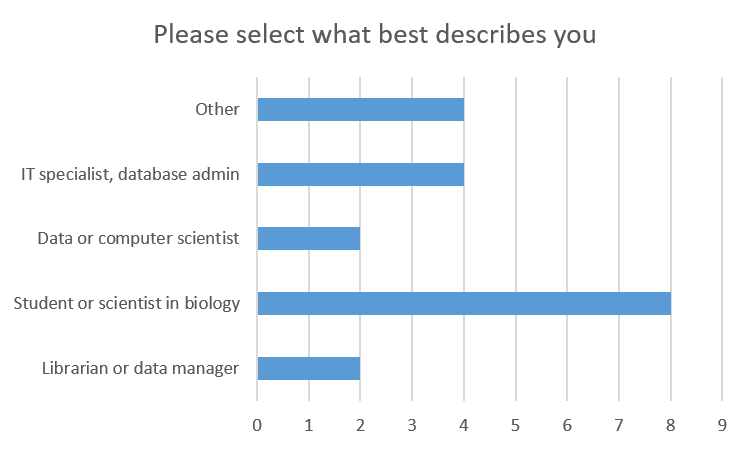
\includegraphics[width=\textwidth]{Figures/webinar-pool}
\decoRule
\caption{Poll results about composition of audience during live participation..}
\label{fig:webinar-poll}
\end{figure}

At the end of the presentation, very interesting questions were raised and discussed. For details, see the ``Results and discussion'' section of this paper.

Larry Page, Project Director at iDigBio, wrote: ``This workflow has the potential to be a huge step forward in documenting use of collections data and enabling iDigBio and other aggregators to report that information back to the institutions providing the data.''

Neil Cobb, a research professor at the Department of Biological Sciences at the Northern Arizona University, suggested that the methods, workflows and tools addressed during the presentation could provide a basis for a virtual student course in biodiversity informatics.

\section{Methods}

Both workflows discussed  rely on three key standards: RESTful API's for the web (\cite{kurtz_what_2013}), Darwin Core (\cite{wieczorek_darwin_2012}), and EML (\cite{fegraus_maximizing_2005}).

RESTful is a software architecture style for the Web, derived from the dissertation of \cite{fielding_architectural_2000}. It is out of the scope of this paper to fully explain what a RESTful API is, but a short summary follows (after \cite{kurtz_what_2013}):

\begin{itemize}
\item{URI's have to be provided for different resources.}
\item{HTTP verbs have to be used for different actions.}
\item{HATEOAS (Hypermedia as the Engine of Application State) must be implemented. This is a way of saying that the client only needs to have a basic knowledge of hypermedia, in order to use the service.}
\end{itemize}

On the other hand, Darwin Core (DwC) is a standard developed by the Biodiversity Information Standards (TDWG), also known as the Taxonomic Databases Working Group, to facilitate storage and exchange of biodiversity and biodiversity-related information. ARPHA and BDJ use the DwC terms to store taxonomic material citation data.

Finally, EML is an XML-based open-source metadata format developed by the community and the National Center for Ecological Analysis and Synthesis (NCEAS) and the Long Term Ecological Research Network (LTER, \cite{fegraus_maximizing_2005}).

\subsection{Development of workflow 1: Automated specimen record import}

There is some confusion about the terms occurrence record, specimen record, and material citation. A DwC Occurrence\footnote{\url{http://rs.tdwg.org/dwc/terms/\#Occurrence}} is defined as ``an existence of an Organism\footnote{\url{http://rs.tdwg.org/dwc/terms/\#Organism}} at a particular place at a particular time.'' The term specimen record is a term that we use for cataloged specimens in a collection that are evidence for the occurrence. In DwC, the notion of a specimen is covered by MaterialSample\footnote{\url{http://rs.tdwg.org/dwc/terms/\#MaterialSample}}, LivingSpecimen\footnote{\url{http://rs.tdwg.org/dwc/terms/\#LivingSpecimen}}, PreservedSpecimen\footnote{\url{http://rs.tdwg.org/dwc/terms/\#PreservedSpecimen}}, and FossilSpecimen\footnote{\url{http://rs.tdwg.org/dwc/terms/\#FossilSpecimen}}. The description of MaterialSample reads: "a physical result of a sampling (or sub-sampling) event. In biological collections, the material sample is typically collected, and either preserved or destructively processed." While there is a semantic difference between an occurrence record (DwC Occurrence) and a specimen record (DwC MaterialSample, LivingSpecimen, PreservedSpecimen, or FossilSpecimen), from the view point of pure syntax, they can be considered equivalent since both types of objects\footnote{We are using the term objects here in the computer science sense of the word to denote generalized data structures.} are described by the same fields in our system grouped in the following major groups:

\begin{itemize}
\item{Record-level information}
\item{Event}
\item{Identification}
\item{Location}
\item{Taxon}
\item{Occurrence}
\item{Geological context}
\end{itemize}

Taxonomic practice dictates that authors cite the materials their analysis is based on in the treatment section of the taxonomic paper (\cite{catapano_taxpub:_2010}). Therefore, in our system, as it is a document-authoring system, we take the view that these objects are material citations, i.e. bibliographic records that refer to a particular observation in the wild or a specimen in a museum. As a Supplementary material 1\footnote{The supplementary files as well as the article itself can be found under \url{https://github.com/vsenderov/idigbio-webinar}.} to the iDigBio article (\cite{senderov_online_2016}), we have attached a spreadsheet listing all DwC terms describing a specimen or occurrence record that can be imported into AWT as a material citation. From here on, we will refer to the objects being imported as specimen records, and to the objects that are part of the manuscript as material citations.

At the time when development of the workflow started, AWT already allowed imp ort of specimen records as material citations via manual interface and via spreadsheet (Suppl. material 1 of \cite{senderov_online_2016}). So, the starting point for the development of the workflow was to locate API's for downloading biodiversity and biodiversity-related data from major biodiversity data providers and to transform the data that was provided by these API's into DwC-compatible data, which was then to be imported into the manuscript. We chose to work with GBIF, BOLD Systems, iDigBio and the PlutoF platform.

In Suppl. material 2 of \cite{senderov_online_2016} we give all the necessary information about the API's and how to map their results to DwC: endpoints, documentation, and the mapping of terms. GBIF and iDigBio name their fields in accordance with DwC, whereas for PlutoF and BOLD Systems there is a direct mapping given in the spreadsheet.

In order to abstract and reuse source code we have created a general Occurrence class, which contains the code that is shared between all occurrences, and children classes GbifOccurrence, BoldOccurrence, IDigBioOccurrence, and PlutoFOccurrence, which contain the provider-specific code. The source code is written in PHP.

\subsection{Development of workflow 2: Automated data paper generation}

Data papers are scholarly articles describing a dataset or a data package (\cite{chavan_data_2011}). Similarly, metadata are data about a dataset (\cite{michener_meta-information_2006}). Ecological metadata can be expressed in an XML-language called EML (\cite{fegraus_maximizing_2005}). It formalizes the set of concepts needed for describing ecological data (\cite{fegraus_maximizing_2005}). It is broad enough and allows dataset authors from neighboring disciplines (e.g. taxonomy) to annotate their datasets with it. We asked ourselves the question: would it be possible to convert such metadata into a data paper manuscript? As the data paper manuscript in AWT is also stored as XML (for format details see the Pensoft API\footnote{Pensoft API available under \url{http://arpha.pensoft.net/dev/}.}), all that was needed was an XSLT transformation mapping the fields of EML to the fields in the data paper XML. We have created two such transformations, for EML version 2.1.1 and for EML version 2.1.0, which we've attached as Suppl. material 3. The workflow has been tested with EML metadata downloaded from GBIF, DataONE and the LTER Network, however, it can be used for EML metadata from any other data provider.

\section{Results and Discussion}

\subsection{Workflow 1: Automated specimen record import into manuscripts developed in the ARPHA Writing Tool}

\subsubsection{Implementation}

It is now possible to directly import a specimen record as a material citation in an ARPHA Taxonomic Paper from GBIF, BOLD, iDigBio, and PlutoF (Slide 5, as well as Fig.~\ref{fig:workflow-idigbio}). The workflow from the user's perspective has been thoroughly described in a blog post; concise stepwise instructions are available via ARPHA's Tips and tricks guidelines. In a nutshell, the process works as follows:

\begin{enumerate}
\item{At one of the supported data portals (BOLD, GBIF, iDigBio, PlutoF), the author locates the specimen record he/she wants to import into the Materials section of a Taxon treatment (available in the Taxonomic Paper manuscript template).}
\item{Depending on the portal, the user finds either the occurrence identfier of the specimen, or a database record identifier of the specimen record, and copies that into the respective upload field of the ARPHA system (Fig.~\ref{fig:occurrence-input-mask}).}
\item{After the user clicks on ``Add,'' a progress bar is displayed, while the specimens are being uploaded as material citations.}
\item{The new material citations are rendered in both human- and machine-readable DwC format in the Materials section of the respective Taxon treatment and can be further edited in AWT, or downloaded from there as a CSV file.}
\end{enumerate}

\begin{figure}
\centering
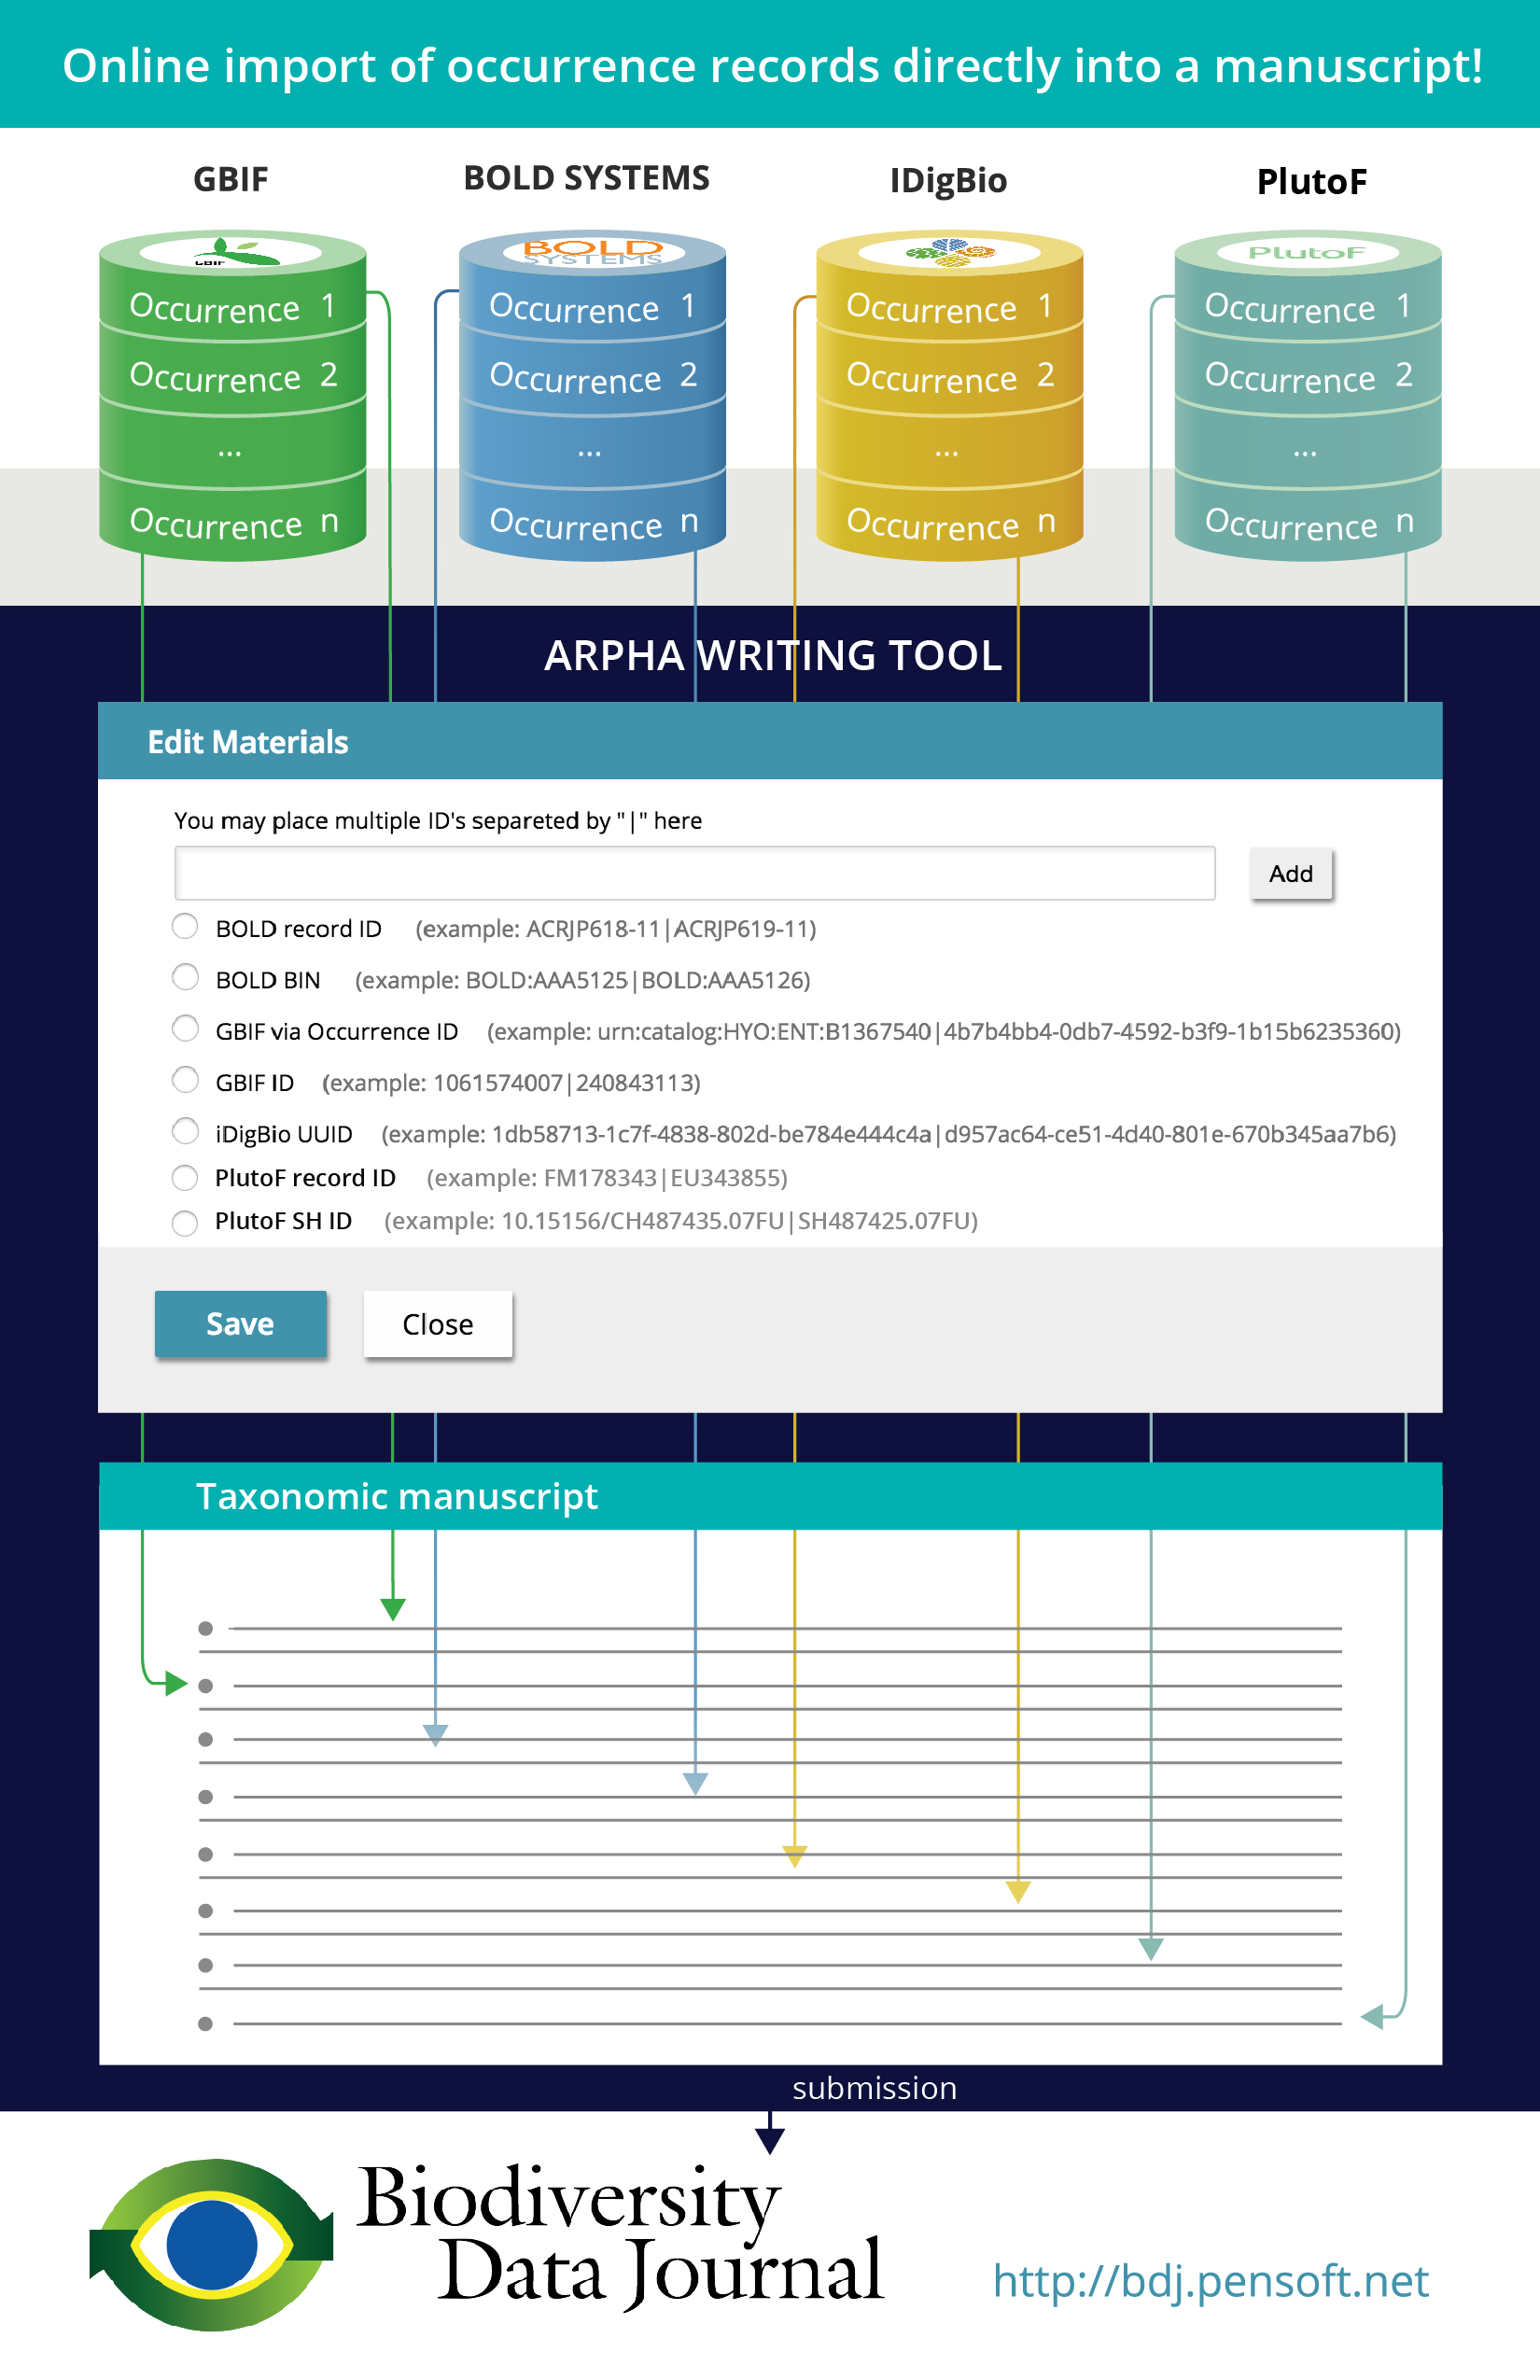
\includegraphics[width=\textwidth]{Figures/workflow-idigbio}
\decoRule
\caption{This fictionalized workflow presents the flow of information content of biodiversity specimens or biodiversity occurrences from the data portals GBIF, BOLD Systems, iDigBio, and PlutoF, through user-interface elements in AWT to textualized content in a Taxonomic Paper manuscript template intended for publication in the Biodiversity Data Journal.}
\label{fig:workflow-idigbio}
\end{figure}

\begin{figure}
\centering
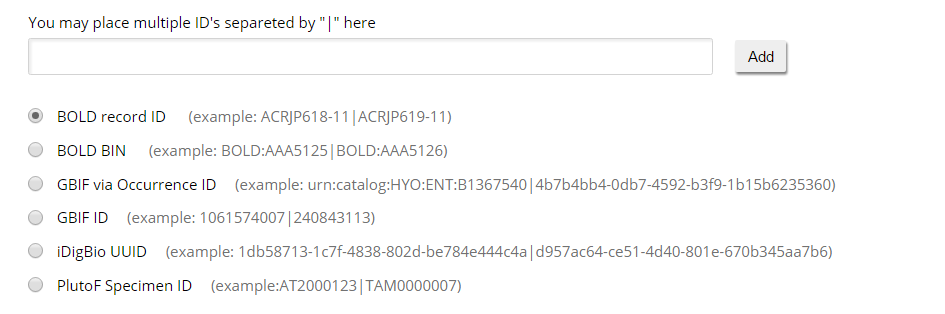
\includegraphics[width=\textwidth]{Figures/occurrence-input-mask}
\decoRule
\caption{User interface of the ARPHA Writing Tool controlling the import of specimen records from external databases.}
\label{fig:occurrence-input-mask}
\end{figure}

\paragraph{Discussion.} The persistent unique identifiers (PID's) are a long-discussed problem in biodiversity informatics (\cite{guralnick_trouble_2014}). Questions of fundamental importance are: given a specimen in a museum, is it (and how often is it) cited in a paper? What about the quality of the database record belonging to this specimen? In order for us to be able to answer these questions to our satisfaction, specimens need to have their own unique identifiers, which are imported as part of the material citation and allow the researcher to scan through the body of published literature to find which specimens have been cited (and how often). In practice, however, this is not always the case and we have to rely on the DwC triplet, ({\tt institutionCode}, {\tt collectionCode}, {\tt catalogNumber}), to positively identify specimens (\cite{guralnick_trouble_2014}). In the next paragraphs, we discuss how the information provided by the repositories can be used to track material citations.

\paragraph{GBIF.} Import from GBIF is possible both via a DwC {\tt occurrenceID}, which is the unique identifier for the specimen/ occurrence, or via a GBIF ID, which is the record ID in GBIF's database. Thanks to its full compliance with DwC, it should be possible to track specimens imported from GBIF.

\paragraph{BOLD Systems.} In the BOLD database, specimen records are assigned an identifier, which can look like {\tt ACRJP619-11}. This identifier is the database identifier and is used for the import; it is not the identifier issued to the specimen stored in a given collection. However, some collection identifiers are returned by the API call and are stored in the material citation, for example, DwC catalogNumber and DwC institutionCode (see mappings in Suppl. material 2 in \cite{senderov_online_2016}). In this case, we have what is called a DwC doublet (\cite{guralnick_trouble_2014}), which provides us with the minimum amount of information to attempt an identification.

A feature of BOLD Systems is that records are grouped into BIN's representing Operational Taxonomic Units (OTU's) based on a hierarchical/ graph-based clustering algorithm (\cite{ratnasingham_dna-based_2013}). It is possible to import all specimen records from a BIN in a single step, specifying the BIN ID. This streamlines the description of new species from OTU's as it allows the taxonomist to save time and import all materials from the BIN.

\paragraph{iDigBio.} iDigBio provides its specimen records in a DwC-compatible format. Similar to GBIF, both a DwC occurrenceID, as well as DwC triplet information is returned by the system and stored in our XML making tracking of specimen citations easy.

\paragraph{PlutoF.} Import from PlutoF is attained through the usage of a specimen ID (DwC catalogNumber), which is disambiguated to a PlutoF record ID by our system. If a specimen ID matches more than one record in the PlutoF system, multiple records are imported and the user has to delete the superfluous material citations. PlutoF does store a full DwC triplet while no DwC occurrenceID is available for the time being.

Ultimately, this workflow can serve as a curation filter for increasing the quality of specimen data via the scientific peer review process. By importing a specimen record via our workflow, the author of the paper vouches for the quality of the particular specimen record that he or she presumably has already checked against the physical specimen. Then a specimen that has been cited in an article can be marked with a star as a peer-reviewed specimen by the collection manager. Also, the completeness and correctness of the specimen record itself can be improved by comparing the material citation with the database record and synchronizing differing fields.

There is only one component currently missing from for this curation workflow: a query page that accepts a DwC occurrenceID or a DwC doublet/ triplet and returns all the information stored in the Pensoft database regarding material citations of this specimen.

\subsection{Workflow 2: Automated data paper manuscript generation from EML metadata in the ARPHA Writing Tool}

\paragraph{Implementation.} We have created a workflow that allows authors to automatically create data paper manuscripts from the metadata stored in EML. The completeness of the manuscript created in such a way depends on the quality of the metadata; however, after generating such a manuscript, the authors can update, edit, and revise it as any other scientific manuscript in the AWT. The workflow has been thoroughly described in a blog post; concise stepwise instructions are available via ARPHA's Tips and tricks guidelines. In a nutshell, the process works as follows:

\begin{enumerate}
\item{The users of ARPHA need to save a dataset's metadata as an EML file (versions 2.1.1 and 2.1.0, support for other versions is being continually updated) from the website of the respective data provider (see Fig.~\ref{fig:EML-download} as an example using the GBIF's Integrated Publishing Toolkit (IPT)). Some leading data portals that provide such EML files are GBIF (EML download possible both from IPT and from the portal), DataONE, and the LTER Network.}
\item{Click on the ``Start a manuscript'' button in AWT and then select ``Biodiversity Data Journal'' and the ``Data paper (Biosciences)'' template (Fig.~\ref{fig:journal-selection}).}
\item{Upload this file via the "Import a manuscript" function on the AWT interface (Fig.~\ref{fig:user-interface}).}
\item{Continue with updating and editing and finally submit your manuscript inside AWT.}
\end{enumerate}

\begin{figure}
\centering
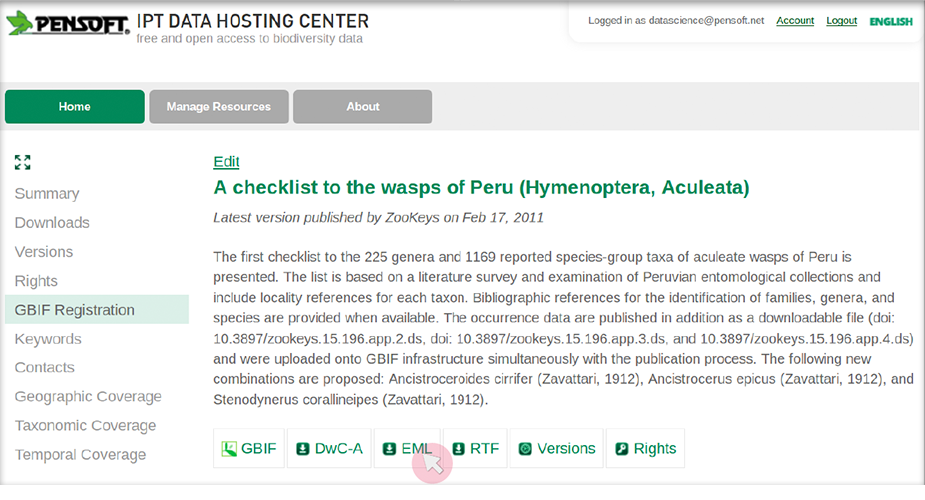
\includegraphics[width=\textwidth]{Figures/EML-download}
\decoRule
\caption{Download of an EML from the GBIF Integarted Publishuing Toolkit (IPT).}
\label{fig:EML-download}
\end{figure}

\begin{figure}
\centering
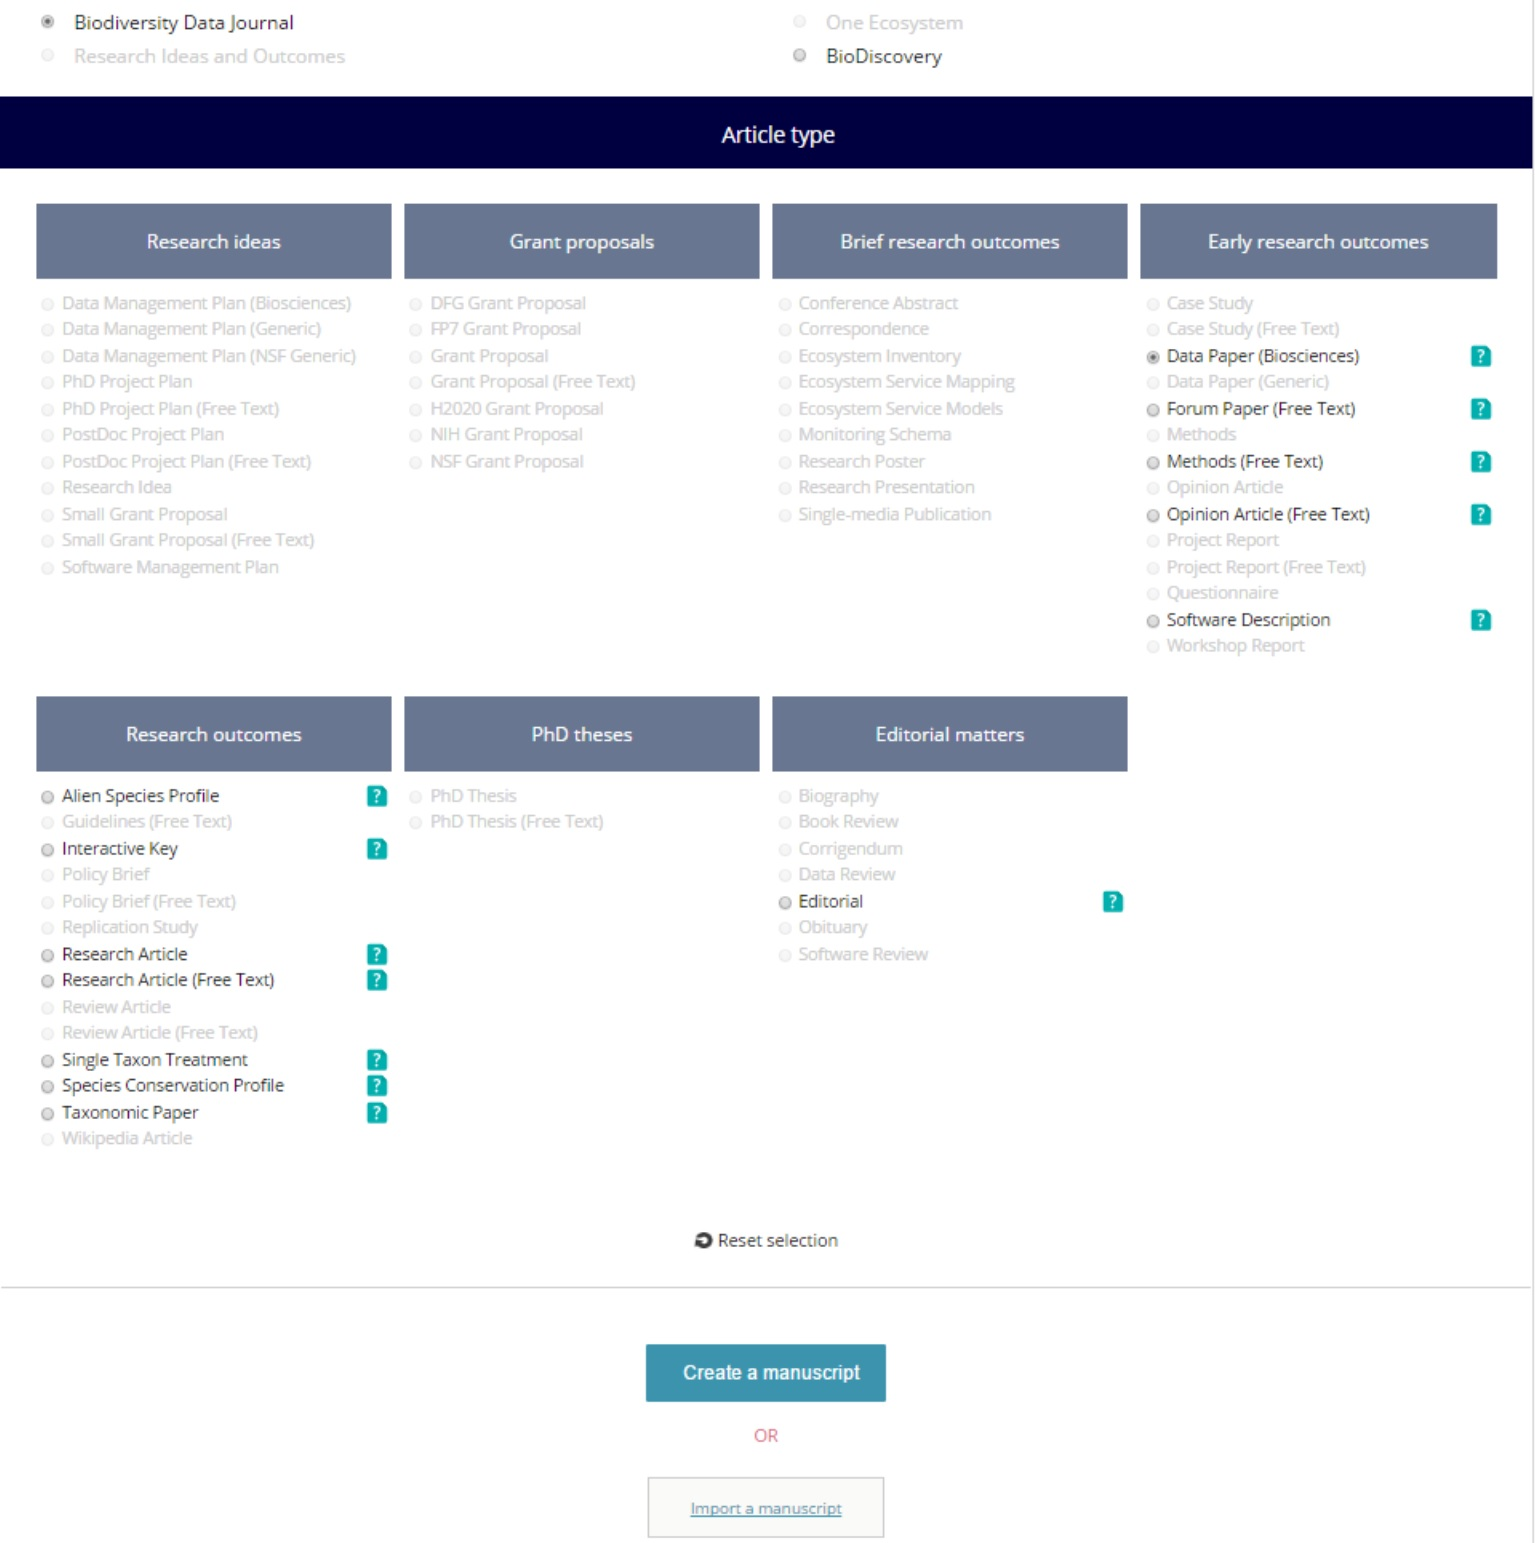
\includegraphics[width=\textwidth]{Figures/journal-selection}
\decoRule
\caption{Selection of the journal and ``Data Paper (Biosciences)'' template in the ARPHA Writing Tool.}
\label{fig:journal-selection}
\end{figure}

\begin{figure}
\centering
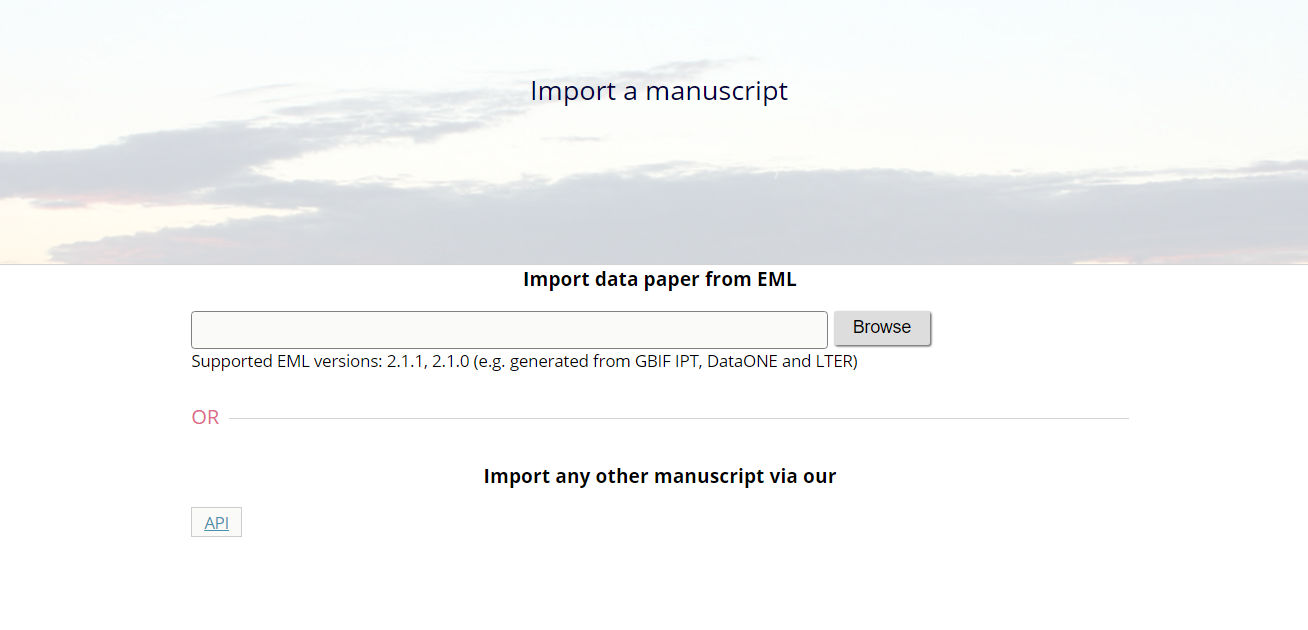
\includegraphics[width=\textwidth]{Figures/user-interface}
\decoRule
\caption{The user interface field for uploading EML files into ARPHA.}
\label{fig:user-interface}
\end{figure}

\paragraph{Discussion} In 2010, GBIF and Pensoft began investigating mainstream biodiversity data publishing in the form of ``data papers.'' As a result this partnership pioneered a workflow between GBIF’s IPT and Pensoft’s journals, viz.: ZooKeys, MycoKeys, Phytokeys, Nature Conservation, and others. The rationale behind the project was to motivate authors to create proper metadata for their datasets to enable themselves and their peers to properly make use of the data. Our workflow gives authors the opportunity to convert their extended metadata descriptions into data paper manuscripts with very little extra effort. The workflow generates data paper manuscripts from the metadata descriptions in IPT automatically at the "click of a button." Manuscripts are created in Rich Text Format (RTF) format, edited and updated by the authors, and then submitted to a journal to undergo peer review and publication. The publication itself bears the citation details of the described dataset with its own DOI or other unique identifier. Ideally, after the data paper is published and a DOI is issued for it, it should be included in the data description at the repository where the data is stored. Within less than four years, a total of more than 100 data papers have been published in Pensoft's journals (examples: \cite{brosens_formidabel:_2013}, \cite{desmet_database_2013}, \cite{gutt_antarctic_2013}, \cite{pierrat_antarctic_2012}, \cite{shao_dataset_2012}, \cite{tng_vegetation_2016}). The workflow and associated author guidelines are described in \cite{penev_pensoft_2016}.

The present chapter describes the next technological step in the generation of data papers: direct import of an EML file via an API into a manuscript being written in AWT. A great advantage of the present workflow is that data paper manuscripts can be edited and peer-reviewed collaboratively in the authoring tool even before submission to the journal. These novel features provided by AWT and BDJ may potentially become a huge step forward in experts' engagement and mobilization to publish biodiversity data in a way that facilitates recording, credit, preservation, and re-use. Another benefit of this usage of EML data might be that in the future, more people wil provide more robust EML data files.

\paragraph{Feedback.} The two workflows presented generated a lively discussion at the end of the presentation, which we summarize below:

\begin{enumerate}
\item{Are specimen records imported from GBIF and then slightly changed during the editorial process then deduplicated at GBIF? Answer: Unfortunately, no. At GBIF, deduplication only occurs for identical records.}
\item{Are we leaving the identifiers from GBIF or iDigBio in the records? Answer: Yes. We have made the best effort to import specimen record identifiers. This has been discussed in the previous sections.}
\item{How will the tool reduce the input time for constructing a manuscript? Answer: AWT reduces the time for creating a manuscript in two significant ways. First of all, the workflows avoid retyping of specimen records or metadata. Secondly, another time-saving feature is the elimination of copying errors. Creating of data paper manuscripts from EML saves, as a minimum, the effort of copy-pasting metadata and their arrangement in a manuscript.}
\item{What are the major hurdles or challenges left in having this become a mainstream tool? How mature is the tool? Answer: We believe that the main hurdles in this becoming a main-stream tool are visibility and awareness of the tool by the community. As the stability of the software is already at a very good stage.}
\item{Is it possible to track the usage of museum specimens for data aggregators? Answer: Yes, see question 2 and discussion in the present section.}
\item{How do you go to the article page where collection managers can search for data published from their collections on the Pensoft website? Answer: We are working on the streamlining of this functionality. It will be part of the OBKMS. Currently, we markup collection codes against the Global Registry of Biodiversity Repositories (GRBio\footnote{GRBio is available under \url{http://grbio.org/}}) vocabularies, and the reader can view the records from a particular collection by clicking on the collection code.}
\end{enumerate}
\include{Chapters/8_Webpportal}
\part{Conclusion}
\label{part:conclusion}
% Chapter Template

\chapter{Summary} % Main chapter title

\label{chapter:summary} % Change X to a consecutive number; for referencing this chapter elsewhere, use \ref{ChapterX}

\section{Contributions of the Thesis}

In the course of the investigative effort, we have made several significant contributions. The two equally important key contributions of the thesis are the creation of an ontology, OpenBiodiv-O (see Chapter~\ref{chapter-ontology}), enabling the linking of biodiversity knowledge on the basis of scholarly publications, and a linked open dataset, OpenBiodiv LOD (see Chapter~\ref{chapter-lod}) consisting of a transformation to Resource Description Framework (RDF) and integration in a single store of information from three major repositories of biodiversity data: the journal databases of Pensoft Publishers and Plazi, and GBIF's taxonomic backbone.

OpenBiodiv-O, serves as the basis of OpenBiodiv-LOD. By developing an ontology focusing on biological taxonomy, our intent is to provide an ontology that fills in the gaps between ontologies for biodiversity resources such as Darwin-SW and semantic publishing ontologies such as the ontologies comprising the SPAR Ontologies. Moreover, we take the view that it is advantageous to model the taxonomic process itself rather than any particular state of knowledge.

After the populating the ontology, we have developed a web-site (see Chapter~\ref{chapter-openbiodiv}, \href{http://openbiodiv.net}{<http://openbiodiv.net>}, containing a semantic search engine and apps running on top of OpenBiodiv LOD.

Furthermore, we have developed two automated workflows---automatic data paper generation and automatic occurrence record import, see Chapter~\ref{chapter-case-study}---between external repositories and the Pensoft database of biodiversity data.

Last but not least is the creation of a framework for transforming XML and CSV files to RDF in the R programming language (RDF4R, see Chapter~\ref{chapter-rdf4r}).

%----------------------------------------------------------------------------------------
%	THESIS CONTENT - APPENDICES
%----------------------------------------------------------------------------------------

\appendix % Cue to tell LaTeX that the following "chapters" are Appendices

% Include the appendices of the thesis as separate files from the Appendices folder
% Uncomment the lines as you write the Appendices

%% Appendix A

\chapter{Frequently Asked Questions} % Main appendix title

\label{AppendixA} % For referencing this appendix elsewhere, use \ref{AppendixA}

\section{How do I change the colors of links?}

The color of links can be changed to your liking using:

{\small\verb!\hypersetup{urlcolor=red}!}, or

{\small\verb!\hypersetup{citecolor=green}!}, or

{\small\verb!\hypersetup{allcolor=blue}!}.

\noindent If you want to completely hide the links, you can use:

{\small\verb!\hypersetup{allcolors=.}!}, or even better: 

{\small\verb!\hypersetup{hidelinks}!}.

\noindent If you want to have obvious links in the PDF but not the printed text, use:

{\small\verb!\hypersetup{colorlinks=false}!}.

%\include{Appendices/AppendixB}
%\include{Appendices/AppendixC}

%----------------------------------------------------------------------------------------
%	BIBLIOGRAPHY
%----------------------------------------------------------------------------------------

\printbibliography[heading=bibintoc]

%----------------------------------------------------------------------------------------

\end{document}  
